\documentclass[12pt,fleqn]{article}
\usepackage{a4}
\usepackage{graphicx}
\usepackage[table,xcdraw]{xcolor}
\graphicspath{ {./Figures/} }
\usepackage{psfrag}
\usepackage{amsmath}                     % \boldsymbol{#1}
\usepackage{amssymb}
\usepackage{Styles/hangcaption}
\usepackage{pstricks}
\usepackage{Styles/pst-node}
\usepackage{Styles/fancyheadings}
\usepackage{tocloft}
\usepackage{cite}
\usepackage{hyperref}
\usepackage[printonlyused]{acronym}
\usepackage{epstopdf}
\usepackage{datetime}
\usepackage{pdfpages}
\usepackage{tabulary}
\usepackage{longtable}
\usepackage[table,xcdraw]{xcolor}
\usepackage{lscape}
\usepackage{float}


\usepackage{capt-of}
\usepackage{array}
\usepackage{colortbl}
\usepackage{rotating}
\usepackage{listings}
\usepackage{setspace}
\definecolor{codegreen}{rgb}{0,0.6,0}
\definecolor{codegray}{rgb}{0.5,0.5,0.5}
\definecolor{codepurple}{rgb}{0.58,0,0.82}
\definecolor{backcolour}{rgb}{0.95,0.95,0.92}

\lstdefinestyle{mystyle}{
    backgroundcolor=\color{backcolour},   
    commentstyle=\color{codegreen},
    keywordstyle=\color{magenta},
    numberstyle=\tiny\color{codegray},
    stringstyle=\color{codepurple},
    basicstyle=\ttfamily\footnotesize,
    breakatwhitespace=false,         
    breaklines=true,                 
    captionpos=b,                    
    keepspaces=true,                 
    numbers=left,                    
    numbersep=5pt,                  
    showspaces=false,                
    showstringspaces=false,
    showtabs=false,                  
    tabsize=2
}

\lstset{style=mystyle}

\newdateformat{monthyeardate}{%
\monthname[\THEMONTH], \THEYEAR}
\hypersetup{
    colorlinks=false,
    linkcolor=black,
    filecolor=black,      
    urlcolor=black,
    }
    
\usepackage{nomencl}
\makenomenclature

\newcommand\Nomenclature[2]{\nomenclature[#2]{#1}{#2}}


% \newcommand{\yesthreeday}{{\AdvanceDate[-4]\today}}
\epstopdfDeclareGraphicsRule{.pdf}{png}{.png}{convert #1\OutputFile}
\DeclareGraphicsExtensions{.png,.pdf}

%-----Tex width---------------------------------
\textwidth 16cm

%-----Line spacing-------------------------------
\renewcommand{\baselinestretch}{1.5}     % 1,1-zeilig

%---------Add dots in TOC-----------------------
\renewcommand{\cftsecleader}{\cftdotfill{\cftdotsep}}

%------Paragraph indention-------------------------------
\setlength{\parskip}{1.5ex plus0.5ex minus0.5ex}

%-----Prevent indent----------------------
\setlength{\parindent}{0em}

%-----Richtiger Abstand fur Einheiten-------------
\def\Unit{\hspace{0.25em}}

%-----Definition of the header--------------------
\pagestyle{fancyplain}
\renewcommand{\sectionmark}[1]{\markboth{Chapter~\thesection.~#1}{#1}}
\renewcommand{\subsectionmark}[1]{\markright{\thesubsection\ #1}}
\rhead[\fancyplain{}{\leftmark}]%
{\fancyplain{\thepage}{\thepage}} \cfoot{} \plainheadrulewidth
0.4pt

\makeatletter
\ifcase \@ptsize \relax % 10pt
  \addtolength{\headheight}{1\p@}
\or % 11pt
  \addtolength{\headheight}{2\p@}
\or % 12pt
  \addtolength{\headheight}{3\p@}
\fi \makeatother

%-----Equations / Figures / Tables numbering according to \ sections
\makeatletter
\renewcommand\theequation{\thesection.\arabic{equation}}
\renewcommand\thefigure{\thesection.\arabic{figure}}
\renewcommand\thetable{\thesection.\arabic{table}}
\@addtoreset{equation}{section} \@addtoreset{figure}{section}
\@addtoreset{table}{section} \makeatother

%-----Useful abbreviations----------------------
\newcommand{\mr}{\mathrm}
\newcommand{\bs}[1]{\mbox{$\boldsymbol{#1}$}}
\newcommand{\degree}[1]{\mbox{$#1^\circ$}}

%------Bibliography style-----------------------
\bibliographystyle{IEEEtran}

%-----Aufzaehlunstiefe im Literaturverzeichnis---------------
\setcounter{tocdepth}{3}

\begin{document}
\pagenumbering{Roman}
\begin{titlepage}
  \begin{center}
      \vspace*{-4.0cm}
    \begin{figure}[!h]
\centering

\includegraphics[width=0.3\linewidth]{Figures/JKUAT_logo.jpg}
\label{fig:jomologo}
\end{figure}
   \large{Jomo Kenyatta University of Agriculture and Technology}\\
    \large{College of Engineering and Technology}\\
    \large{School of Mechanical, Materials, and Manufacturing Engineering}\\
   \large{Department of Mechatronic Engineering}\\
    ------------------------------------------------------------------------------------------------\\[0.1cm]
    \LARGE{\textbf{Design and Fabrication of an Automated Discharge Collection Unit for the Synthetic Hydro-experimental Machine.}}\\[0.1cm]
    \LARGE{\textbf{FYP-18-03}}\\[0.4cm]
    \LARGE{\textbf{FINAL REPORT}}\\[0.4cm]
    \large{\textbf{Juma Joel Mwimali (ENM221-0060/2017)}}\\[0.2cm]
    \large{\textbf{Kipng'eno Erick  (ENM221-0068/2017)}}\\[0.2cm]
     \large{\textbf{Supervisor}}\\
	\large{Dr. Anthony Muchiri}\\
    \large{\small{\monthyeardate\today}}\\
        ------------------------------------------------------------------------------------------------\\
    \small{Submitted in partial fulfillment of the requirements for the degree of Bachelor of Science in Mechatronic Engineering at Jomo Kenyatta University of Agriculture and Technology, 2022}\\
  \end{center}
\end{titlepage}


\addcontentsline{toc}{section}{Declaration}
\section*{Declaration}


We hereby declare that the work contained in this report is original, researched and documented by the undersigned students. It has not been used or presented elsewhere in any form for award of any academic qualification or otherwise. Any material obtained from other parties have been duly acknowledged. We have ensured that no violation of copyright or intellectual property rights have been committed.
\begin{enumerate}
	\item Juma Joel Mwimali \vspace*{.2cm}\\
	Signature\ldots\ldots\ldots\ldots\ldots\ldots\ldots\ldots\ldots\ldots Date\ldots\ldots\ldots\ldots\ldots\ldots\ldots\ldots\ldots\ldots
	\item Kipng'eno Erick \vspace*{.2cm}\\
	Signature\ldots\ldots\ldots\ldots\ldots\ldots\ldots\ldots\ldots\ldots Date\ldots\ldots\ldots\ldots\ldots\ldots\ldots\ldots\ldots\ldots
\end{enumerate}

\vspace*{1cm}
Approved by:\\
\textbf{Supervisor: } Dr. Anthony Muchiri\vspace*{.2cm}\\
Signature\ldots\ldots\ldots\ldots\ldots\ldots\ldots\ldots\ldots\ldots Date\ldots\ldots\ldots\ldots\ldots\ldots\ldots\ldots\ldots\ldots

\textbf{Technologist: } Mr. Mbugua\vspace*{.2cm}\\
Signature\ldots\ldots\ldots\ldots\ldots\ldots\ldots\ldots\ldots\ldots Date\ldots\ldots\ldots\ldots\ldots\ldots\ldots\ldots\ldots\ldots



\clearpage
\lhead{Abstract}
\addcontentsline{toc}{section}{Abstract}
\section*{Abstract}
\label{sec:}
\par
The synthetic hydro-experimental machine used for fluid mechanics experiments in the fluids lab at JKUAT uses a manual mechanical system for the collection of the discharge during experiments such as the determination of the coefficient of discharge of the Venturi and the orifice. During such experiments, the user is required to turn the main discharge ball valve in steps determined by human intuition, and for every step, they are required to slide a metallic diverter to collect the discharge to a separate tank, and at the same time, to start measuring the temperature of the discharge, and the timer using an analog stopwatch. This synchronism is necessary for precise data in the computation of the fluid flow properties but cannot be achieved by humans. 
\par
The design and fabrication of an automated discharge collection unit intended to reduce human error by approximately 10\% have been outlined in this report. The design was modularised into three units; a discharge flow control unit, a discharge handling unit, and an interface and a control unit. The discharge flow control unit was designed to control the main ball valve in steps of less than $1^0$ using a servo motor and divert the flow in less than 1.5 seconds using a linear actuator. The discharge handling unit was also designed with a tank that can collect up to 25 kg of discharge. The tank was also fitted with automated temperature and weight measurement units. The interface was designed on a touch LCD running on an STM32 microcontroller.
\par
This automation results in a reduction of the gross error by 8.213 \%.
\clearpage
\tableofcontents
\clearpage
\addcontentsline{toc}{section}{Table of Contents}
\lhead{List of Figures}
\addcontentsline{toc}{section}{List of Figures}
\let\oldnumberline\numberline%
\renewcommand{\numberline}{\figurename~\oldnumberline}%
\listoffigures
\clearpage
\lhead{List of Tables}
\renewcommand{\numberline}{\tablename~\oldnumberline}%
\listoftables
\newpage
\clearpage
\lhead{Nomenclature}
\addcontentsline{toc}{section}{Nomenclature}
\Nomenclature{GPIO}{General Purpose Input Output}
\Nomenclature{CFD}{Computational Fluid Dynamics}
\Nomenclature{SKE}{Single Kernel Estimate}
\Nomenclature{MAWS}{Marine Automatic Water Sampler}
\Nomenclature{UMV}{Unmanned Marine Vehicle}
\Nomenclature{RTOS}{Real Time Operating System}
\Nomenclature{GPIO}{General Purpose Input and Output Pins}
\Nomenclature{API}{Application Programming Interface}
\Nomenclature{FSMC}{Flexible Static Memory Controller}
\Nomenclature{MOSFET}{Metal Oxide Field Effect Transistor}
\printnomenclature
\clearpage
\newpage

\clearpage
\pagenumbering{arabic}
  \lhead{Chapter 1. Introduction}
  \section{Introduction}
\label{sec:introduction}
\subsection{Background}
Fluid flow measurement involves the measurement of the properties of a smooth and uninterrupted stream of flowing particles that conform to a pipe. These flow properties include the coefficient of discharge, mass flow rate, fluid velocity, differential pressure, and conductivity coefficients \cite{pereira2009flow}. They are altered and measured by flow measuring devices such as the Venturi, the Orifice, turbine flow meters and rotameters \cite{nandagopal2022fluid}. These measurements are finally related to the flow using the Bernoulli's equation. 

\par
The Synthetic Hydro-Experimental machine, currently installed in JKUAT, is a configurable machine with these flow meters. This machine is used to conduct experiments to establish relationships between the fluid flow properties and the behavior of the flow. It has a lift pump, gate valves, alcohol manometers, pressure gauges, a Pelton turbine, a Venturi, an orifice, and water reservoirs.  During experiments, the lift pump is turned on, and the discharge valve is fully opened to establish a steady flow.  The discharge valve is then closed. The valve is opened in small steps depending on the number of steps required. For each step, the discharge is collected, and its temperature is measured within a specific time interval. Finally, the weight of the collected discharge is also measured.

\subsection{Problem statement}

In fluid flow experiments utilizing the Venturi and the orifice to establish the coefficient of discharge, the discharge steps must be precisely opened, time and temperature measurements must be made concurrently with discharge collection so as to achieve values that are within a reasonable range.The Synthetic Hydro-Experimental machine now in use at JKUAT to establish this relationship, however, is entirely mechanical, making it impossible for a human to do some of the simultaneous measurements. A ball valve regulates the flow rate in small intervals using human intuition, which can be imprecise. As a result, with these discrepancies, the findings might frequently be outside of the acceptable range. Automating the discharge collection process can minimize the error in the results and still preserve the credibility of the experiment.

\subsection{Objectives}
\subsubsection{Main objective}

 To automate the discharge collection process for the Synthetic Hydro-Experimental machine. 

\subsubsection{Specific objectives}

\begin{enumerate}
	\item To design an automated discharge flow control unit that can turn the ball valve in steps of less than $1^{0}$ and divert the flow in less than 1 second. Turning of less than $1^{0}$ ensures more runs of experiment can be conducted.
	\item To design and fabricate a discharge handling unit with automated weight, time and temperature measurements, and a discharge collection tank that can discharge within 2 seconds.
    \item To design a graphical user interface and a robust control algorithm to integrate the units.

\end{enumerate}

\subsubsection{Expected outcomes}
A unit with a discharge flow control mechanism that can turn in steps of less than $1^{0}$. Furthermore, to accurately regulate the flow of the discharge into either the collecting tank or into the main reservoir, the mechanism should be able to divert the flow from the pipeline in less than a second. The discharge should then be collected in a  tank that can store up to $0.02m^{3}$ of the discharge. A weight measurement device with a gauge factor of more than 2 to be attached at the bottom of the collection tank. A graphical user interface that allows for the displaying of measurements in this case temperature, time and weight and control of operations

% \begin{enumerate}
%     \item \textbf{Discharge flow control unit}
%     \begin{itemize}
%         \item \textbf{Flow control subunit}-  A discharge flow control mechanism that can turn steps less than $1^{0}$. This is necessary in a case where an experiment is to be done in more than 90 steps( less than $1^{0}$ per step). 
%         \item \textbf{Diversion subunit} - A mechanism that can divert the flow in less than a second. This is to ensure that only the flow within the time interval is collected.
%     \end{itemize}
%     \item \textbf{Discharge Handling unit}
%     \begin{itemize}
%         \item \textbf{Discharge collection tank}  - A tank that can collect up to $0.02m^{3}$ of the discharge. This is an estimated quantity of the discharge collected when the valve is fully open for approximately 30 seconds.
%         \item \textbf{Discharge Weight measurement} -  A weight measurement device with a gauge factor of more than 2. This is necessary to detect even the smallest change in weight.
%         \item \textbf{Discharge temperature measurement} - An immersible temperature sensor with a resolution of more than 10 bits. This is necessary to detect even the smallest change in the temperature of the discharge.
%         \item \textbf{Outlet valve} - Approximately 1 inch valve in order to empty the empty approximately $0.02m^{3}$ in the least time possible. 
%     \end{itemize}
%     \item \textbf{Interface and Control Unit}
%     \begin{itemize}
%         \item \textbf{Micro-controller} - A microcontroller that can drive a 320x240 touch LCD at approximately 30 frames per second. This is to ensure the displayed data is updated on time while maintaining a slick graphical user interface. 
%         \item \textbf{Application logic} - A robust application logic with auto-calibration capabilities, and event-driven. 
%     \end{itemize}

% \end{enumerate}

\subsection{Justification}
This automation will streamline the discharge collecting process while also ensuring the consistency and quality of the data collected in each phase of the fluid flow tests performed on the system. In contrast to the existing condition, such automation allows a single person to perform the experiment without significant effort. Furthermore, the automated system will also be modular, allowing it to be readily attached and detached from the main machine with few modifications.

  \clearpage
  \lhead{Chapter 2. Literature Review}
  \section{Literature Review}
\subsection{Introduction}
Fluid flow experiments involve determination of the flow velocity, the mass flow rate or volumetric flow rate. These experiments are used to familiarize the students with typical methods of flow measurement of an incompressible fluid and, at the same time demonstrate applications of the Bernoulli's equation. Thus, these experimental investigations require the application of measuring techniques to yield quantitative information on the relationship between pressure, temperature and local flow velocities.
\par
The synthetic hydro-experimental machine employs the use of the venture and the orifice meter in determining these fluid properties specifically the coefficient of discharge. It involves determining the relationship between a flowing fluid through a valve, the weight and temperature of the collected discharge. The machine comprises of four main parts; the diverter, gate valve, weight and temperature measurement unit. The measurement involves four main processes, discharge collection, diversion, weight and temperature measurement. 
\subsubsection{Gate Valve }
\par
The valve is attached at the end of the pipeline immediately after the venture and the orifice meter. It is used in flow rate control by either increasing or reducing the aperture at which the fluid flows. The experiment is conducted in several steps which is determined by opening and closing of the valve. At the start of the experiment, the valve is initially closed hence no fluid is collected. Depending on the required number of steps, the valve is then opened in small steps allowing the discharge to be collected for purposes of weight and temperature measurement.
\subsubsection{Diverter }
\par
After each step of the experiment, the collected fluid flows into the weight measurement unit through the help of a diverter. The diverter is used to direct the collected discharge into the weight measurement unit which is located at the periphery of the rig to avoid flowing back into the reservoir. The diverter is a mechanical device that is moved by hand.
\subsubsection{Temperature measurement unit }
\par
 The temperature of the collected discharge is measured immediately after the fluid flows through the gate valve by use of a thermometer. This is to minimize the environmental effects, for instance the effects of the metallic diverters which would otherwise compromise on the temperature readings. The readings are measured and recorded after each step of the experiment.
\subsubsection{Pressure measurement }
\par
The differential manometers are attached just before and after both the venture and the orifice and is used to determine the pressure of the flowing fluid. These manometric readings are recorded after each and every step of the experiment.
\subsubsection{Weight measurement unit }
\par
The final part involves measuring the weight of the collected discharge. This is done by use of a measuring scale with loads attached to it. The above measurements are then used to establish the coefficient of discharge of the fluid.
\subsection{Existing Technologies}
Some advanced and even rudimentary technologies have been used in place of the Synthetic Hydro-Experimental machine for the determination of fluid flow properties. The technologies include :   
\subsubsection{Computational Fluid Dynamics}
Computational fluid dynamics(CFD) is a powerful modelling and analysis technique that utilizes finite difference techniques to solve highly non-linear differential equation of pressure, energy, relative humidity, air temperature and velocity \cite{raman2018review}. It can be used to model fluid flow in flow measurement devices.
\par
Tukimin et al \cite{tukimin2016cfd} in their study  conducted a CFD analysis using an Single Kernel Estimate (SKE) turbulence model to determine the coefficient of discharge of a Venturi tube, and finally compared the results to those obtained from a physical experimental setup. The test loop shown in figure \ref{fig:test_loop_rig} was used both in a physical setup and a CFD model. 

\begin{figure}[ht]
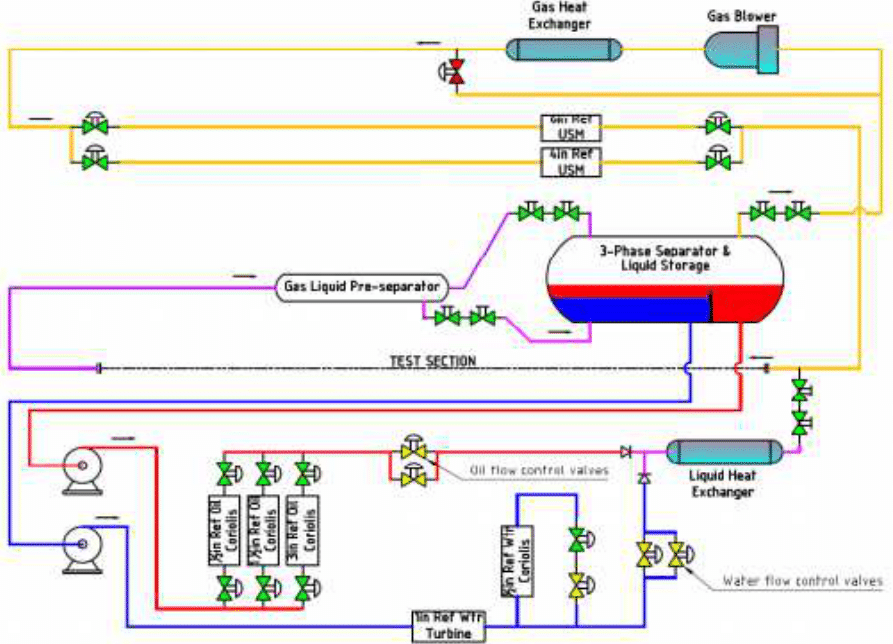
\includegraphics[width=0.9\linewidth]{Figures/test_loop}
\centering
\caption[Test loop schematic]{ Test loop schematic by Tukimin et al \cite{tukimin2016cfd}}
\label{fig:test_loop_rig}
\end{figure}

They designed a CFD model using the ANSYS Design Modeller software. The model consists of a Venturi tube, designed according to the standards ISO 5167:2003 \cite{carello2013flow}, and a liquid and gas system. They did a physical experiment using the same test matrix used in the numerical simulation model. Finally, they computed the coefficient of discharge of the venturi using equation \ref{eq:2}.  

\begin{equation}
C d=\frac{4 m \sqrt{1-\beta^{4}}}{\pi \varepsilon d^{2} \sqrt{200000 D p_{1} \rho_{1}}}
\label{eq:2}
\end{equation}

\begin{table}[!t]
  \begin{center}
    \leavevmode
    \hangcaption{ Calculated $C_{d}$}   
     \begin{tabular}{rlc}\hline
      Venturi under Test & Average Discharge Coefficient &  Average Discharge Coefficient \\ \hline
       & From experiment &  From CFD post \\ \hline
      Venturi 1 & 0.99366 &  0.984347 \\ \hline
    \end{tabular}
    \label{tab:cd}
  \end{center}
\end{table}
The results obtained in \ref{tab:cd} showed a difference of less than $1 \%$ between the $C_{d}$ obtained from the two setups.
\par
Tamhankar et al \cite{tamhankar2014experimental} also did a similar experiment using a CFD model designed in ANSYS Fluent 13.0 utilizing a Realizable k-$\epsilon$ turbulence model which is superior to a Standard k-$\epsilon$ turbulence model and compared the results to those obtained from an experimental setup show in figure \ref{fig:exp}. 


\begin{figure}[H]
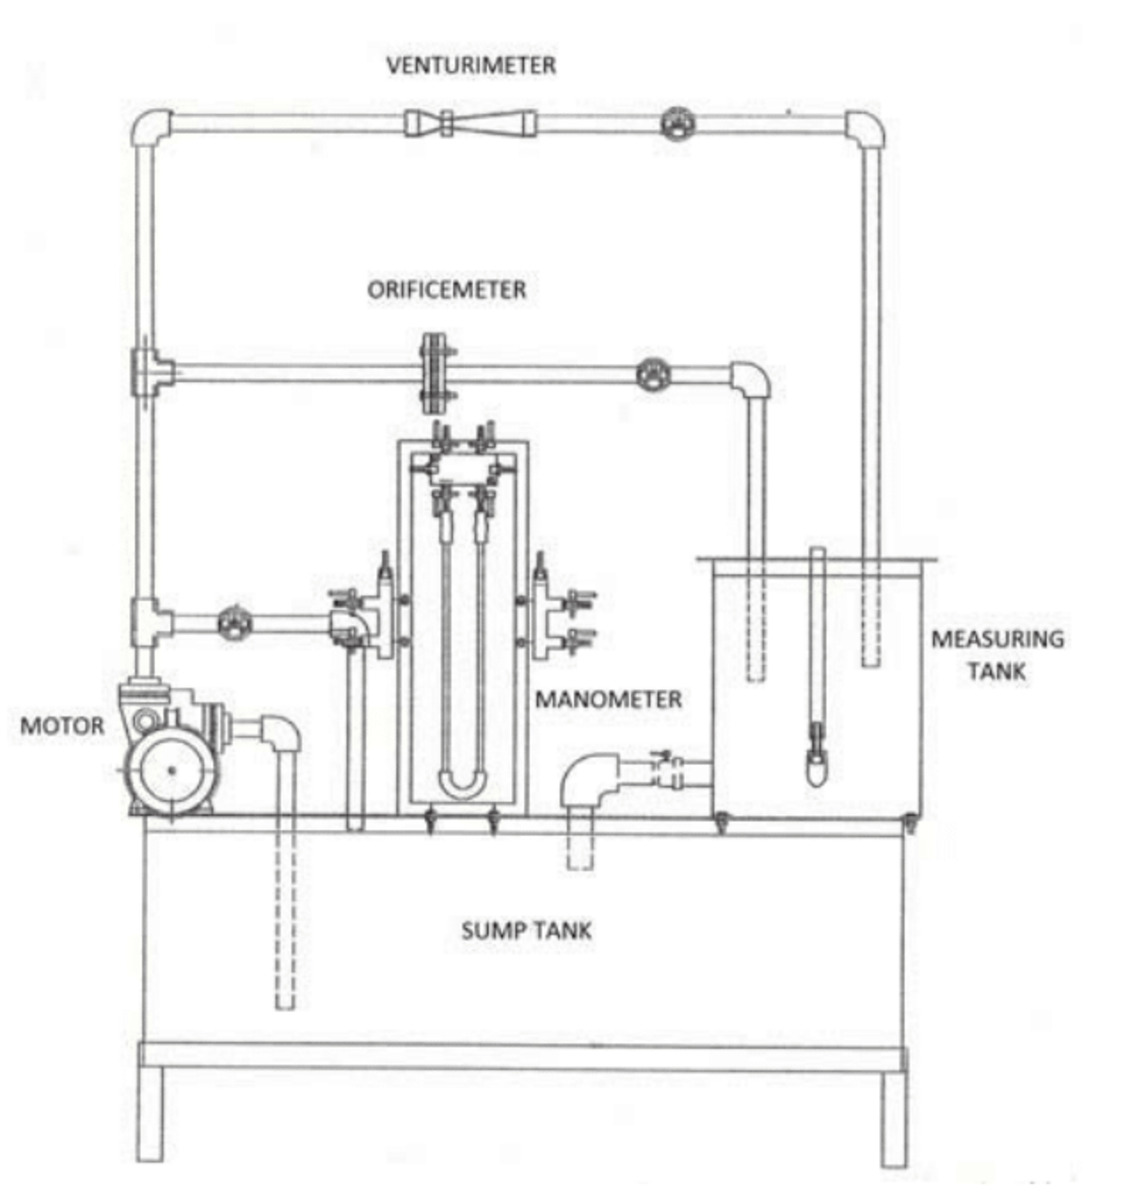
\includegraphics{Figures/exp.jpg}
\centering
\caption[Experimental setup ]{ Experimental setup by Tamhankar et al \cite{tamhankar2014experimental}}
\label{fig:exp}
\end{figure}

Table \ref{tab:results} shows the results obtained from the study
\begin{table}[!t]
    \centering
    \hangcaption{Results}
    \begin{tabular}{|c|c|c|}
        \hline \text { Reading No. } & \text { Experiment } & \text { CFD analysis } \\
        \hline 1 & 0.9724 & 0.9619 \\
        \hline 2 & 0.9592 & 0.9689 \\
        \hline 3 & 0.9779 & 0.9692 \\
        \hline
    \end{tabular}
    \label{tab:results}
\end{table}

The study concluded that difference in values of the coefficient of discharge obtained from the model and those obtained from the experimental setup was less than $ 5 \%$ .
\subsubsection{Analytical Predictions}
This technique utilizes the Bernoulli's equation to establish an analytical correlation between the fluid flow and the coefficient of discharge of the Venturi meter. 

\begin{figure}
    \centering
    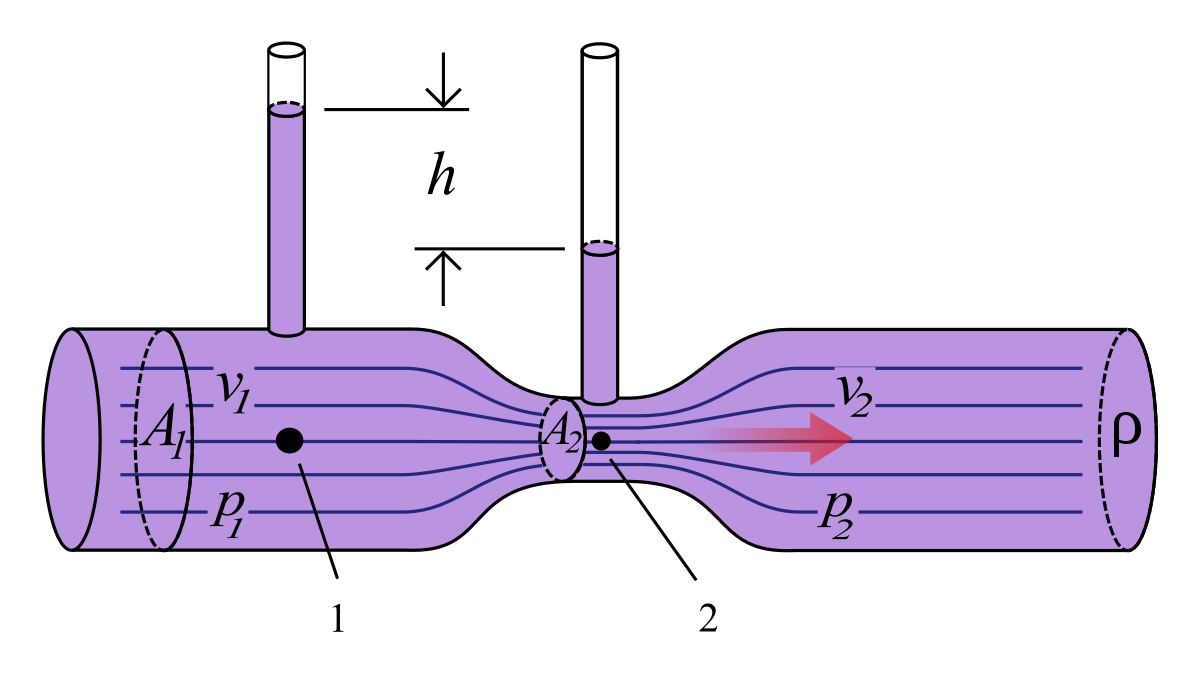
\includegraphics[width=0.6\textwidth]{Figures/venturi}
    \caption[Venturi Meter]{Venturi meter \cite{venturi_meter}}
    \label{fig:venturi}
\end{figure}

Figure \ref{fig:venturi} shows the Venturi meter. Assuming the flow is ideal and applying the Bernoulli's equation before and after the contraction, 

\begin{equation}
\begin{aligned}
&\frac{p_{1}}{\rho g}+\frac{v_{1}^{2}}{2 g}+z_{1}=\frac{p_{2}}{\rho g}+\frac{v_{2}^{2}}{2 g}+z_{2} \\
&\text { But } Z_{1}=Z_{2}, \\
&\frac{\left(p_{1}-p_{2}\right)}{\rho}=\frac{\left(v_{2}^{2}-v_{1}^{2}\right)}{2} \\
&\frac{\left(p_{1}-p_{2}\right)}{\rho}=\frac{v_{2}^{2}}{2}\left(1-\frac{A_{2}^{2}}{A_{1}^{2}}\right) \\
&\frac{\Delta p}{\rho}=\frac{v_{2}^{2}}{2}\left(1-\beta^{4}\right) \\
&v_{2}=\frac{1}{\sqrt{1-\beta^{4}}} \sqrt{\frac{2 \Delta p}{\rho}}
\end{aligned}
\label{eq:bernoulli_der}
\end{equation}

Applying the continuity equation to the result of the derivation in \ref{eq:bernoulli_der},
\begin{equation}
\begin{aligned}
&Q_{t h}=A_{1} v_{1}=A_{2} v_{2} \\
&Q_{t h}=A_{2} v_{2}=\frac{1}{\sqrt{1-\beta^{4}}} \frac{\pi d^{2}}{4} \sqrt{\frac{2 \Delta p}{\rho}}
\end{aligned}
\label{eq:mass_flow_rate}
\end{equation}
Equation \ref{eq:mass_flow_rate} of theoretical flow rate is based on the assumption that the flow is steady, incompressible, inviscid, irrotational, no losses and the velocities $V_{1}$ and  $V_{2}$ are constant across the cross section \cite{arun2015prediction}. 

\begin{equation}
\mathrm{Q}_{\mathrm{act}}=\frac{\mathrm{C}_{\mathrm{d}_{\mathrm{st}} \mathrm{d}}}{\sqrt{1-\beta^{4}}} \frac{\pi \mathrm{d}^{2}}{4} \sqrt{\frac{2 \Delta \mathrm{p}}{\rho}}
\end{equation}
The frictional and viscous losses in a laminar flow can be estimated by the Darcy's law
\begin{equation}
\mathrm{H}_{\mathrm{L}}=\frac{(\Delta \mathrm{p})_{\text {viscous }}}{\rho \mathrm{g}}=\mathrm{f} \frac{\mathrm{v}^{2}}{2 \mathrm{~g}} \frac{\mathrm{D}}{\mathrm{D}}
\end{equation}
where 'f' is the friction factor.
\par
Coefficient of discharge equation \ref{eq:cd2} where for laminar flow, 'f' is given by equation \ref{eq:f} . This equation is derived from both the Darcy's law equation and the theoretical flow rate equation \ref{eq:mass_flow_rate}.
\begin{equation}
f=\frac{64}{R_{e d}}
\label{eq:f}
\end{equation}


\begin{equation}
C_{\mathrm{d}}=0.995 \sqrt{\frac{1}{(1+3 f)}}
\label{eq:cd2}
\end{equation}

\par
Arun et al \cite{arun2015prediction} did  a comparision of the $C_{d}$ obtained by this method and that obtained from a CFD simulation. The study concluded that the results from the two methods had an uncertainty of $0.9\%$.
\subsection{Related Works}
Discharge collection techniques have been developed for various applications. Some of these applications are related to the discharge collection unit used in the Synthetic Hydro-Experimental machine.

\subsubsection{Electromagnetic activation}
Angelo et al \cite{odetti2019design} implemented this technique in the design and testing of an Modular Automatic Water Sampler(MAWS). They designed MAWS and mounted them on unmanned marine vehicle with the aim of collecting water samples for scientific campaigns in front of polar tidewater glaciers. Their main design considerations was the response time of the stopper since the MAWS were operated under water and at the risk of damage by glaciers. The actuation unit of the sampler is shown in figure \ref{fig:stopper}. 

\begin{figure}[H]
    \centering
    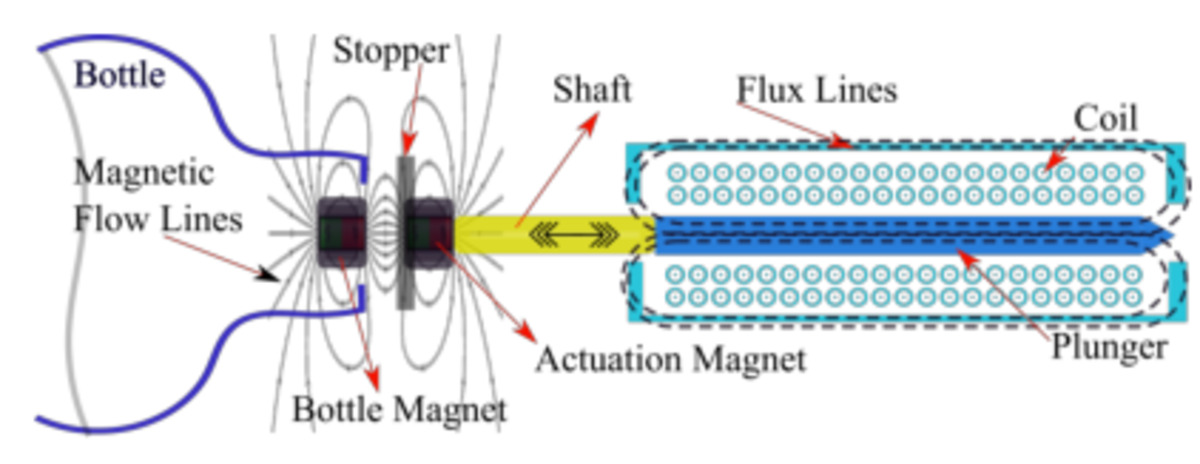
\includegraphics[width=\textwidth]{Figures/stopper.jpg}
    \caption[Sampler actuation mechanism]{Sampler actuation mechanism \cite{odetti2019design}}
    \label{fig:stopper}
\end{figure}

When the coil in the solenoid is crossed by a current a strong magnetic field is generated that attracts the ferromagnetic plunger connected to the sealing stopper and opens the bottle allowing water to flow into the bottle's neck. As the current stops the two permanent magnets attract each other and the stopper seals the bottle \cite{odetti2019design}.

\subsubsection{Pneumatic Control}
Pneumatic actuators utilizes the power of compressed air to impart motion on objects. Sangmin and Joonwon \cite{lee2009development} did a design of cartridge-type pneumatic dispenser with a back flow stopper. The system used a membrane covering a discharge hole. The membrane was opened and closed using negative and positive pneumatic pressure respectively as shown in figure \ref{fig:dispensing_mechanisml}. 

\begin{figure}
    \centering
    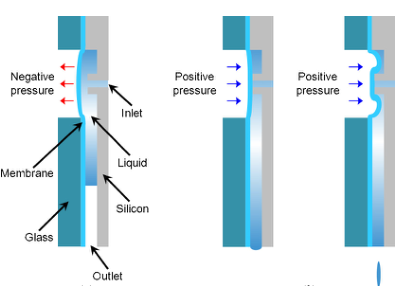
\includegraphics{Figures/dispensing_mechanism.png}
    \caption[Dispensing mechanism]{Dispensing mechanism \cite{lee2009development}}
    \label{fig:dispensing_mechanisml}
\end{figure}

The application was able to do precise dispensation of 100nL to 400nL droplets.

\subsection{Summary}

Every fluid flow experiment done on the Synthetic Hydro-Experimental machine involves the collection of discharge and the measurement of its properties. The most common experiment is the determination of the coefficient of discharge  of the Venturi and the Orifice. In this literature, other techniques such as CFD and analytical methods have been found to be effective as alternatives to this machine. These techniques have been proven to produce results with a difference of less than $1\%$  from the experimental results obtained from a physical setup. Such results can also be obtained from the fluids rig currently used in JKUAT by automating the discharge collection unit. With regard to this, the literature has also covered discharge collection techniques that have proven to be effective in other applications and can be adapted for this automation. This techniques include the application of pneumatics and electromagnetism. 

\subsection{Gap analysis}
\begin{enumerate}
    \item The use of the CFD method undermines the credibility of the fluid flow experiments. This is because CFD mainly involves simulation. Furthermore, the technique technique is rather used for the design of fluid flow measuring devices.
    \item CFD method can also be very resource intensive in terms of compute resources. Softwares used for this method requires a hefty license fee.
    \item The application of the analytical method involves tedious calculations and several assumptions which can produce untrustworthy results.
    \item The use of the Synthetic Hydro-Experimental machine with a manual discharge collection unit often produce results with huge error margins (73 percent).  
\end{enumerate}

This project is entirely focused on addressing gap number four with the application of techniques such as pneumatics or electromagnetism. This closes in the technological gap with the use of CFD, and simplify the use of analytical methods by providing data for the computation of fluid flow properties.    






  \clearpage
  \lhead{Chapter 3. Methodology}
    \section{Methodology}
\subsection{Overview}
This project consists of three main units: a discharge flow control unit, a discharge handling  unit, and a software and control unit. 
\subsection{Discharge flow control unit}
This unit consist of two main sub-units:
\begin{enumerate}
    \item \textbf{Flow control sub-unit} -
   It controls the dispensing of the discharge from the discharge pipe in steps.
    \item \textbf{Flow diversion sub-unit} -
    It diverts the discharge from the main discharge pipe either to the discharge collection tank or to the main reservoir.
\end{enumerate}
\par
\subsubsection{Flow control  sub-unit}
The current state-of-art of this unit is as shown in Figure \ref{fig:current_discharge_control_unit}. 
\begin{figure}[H]
    \centering
    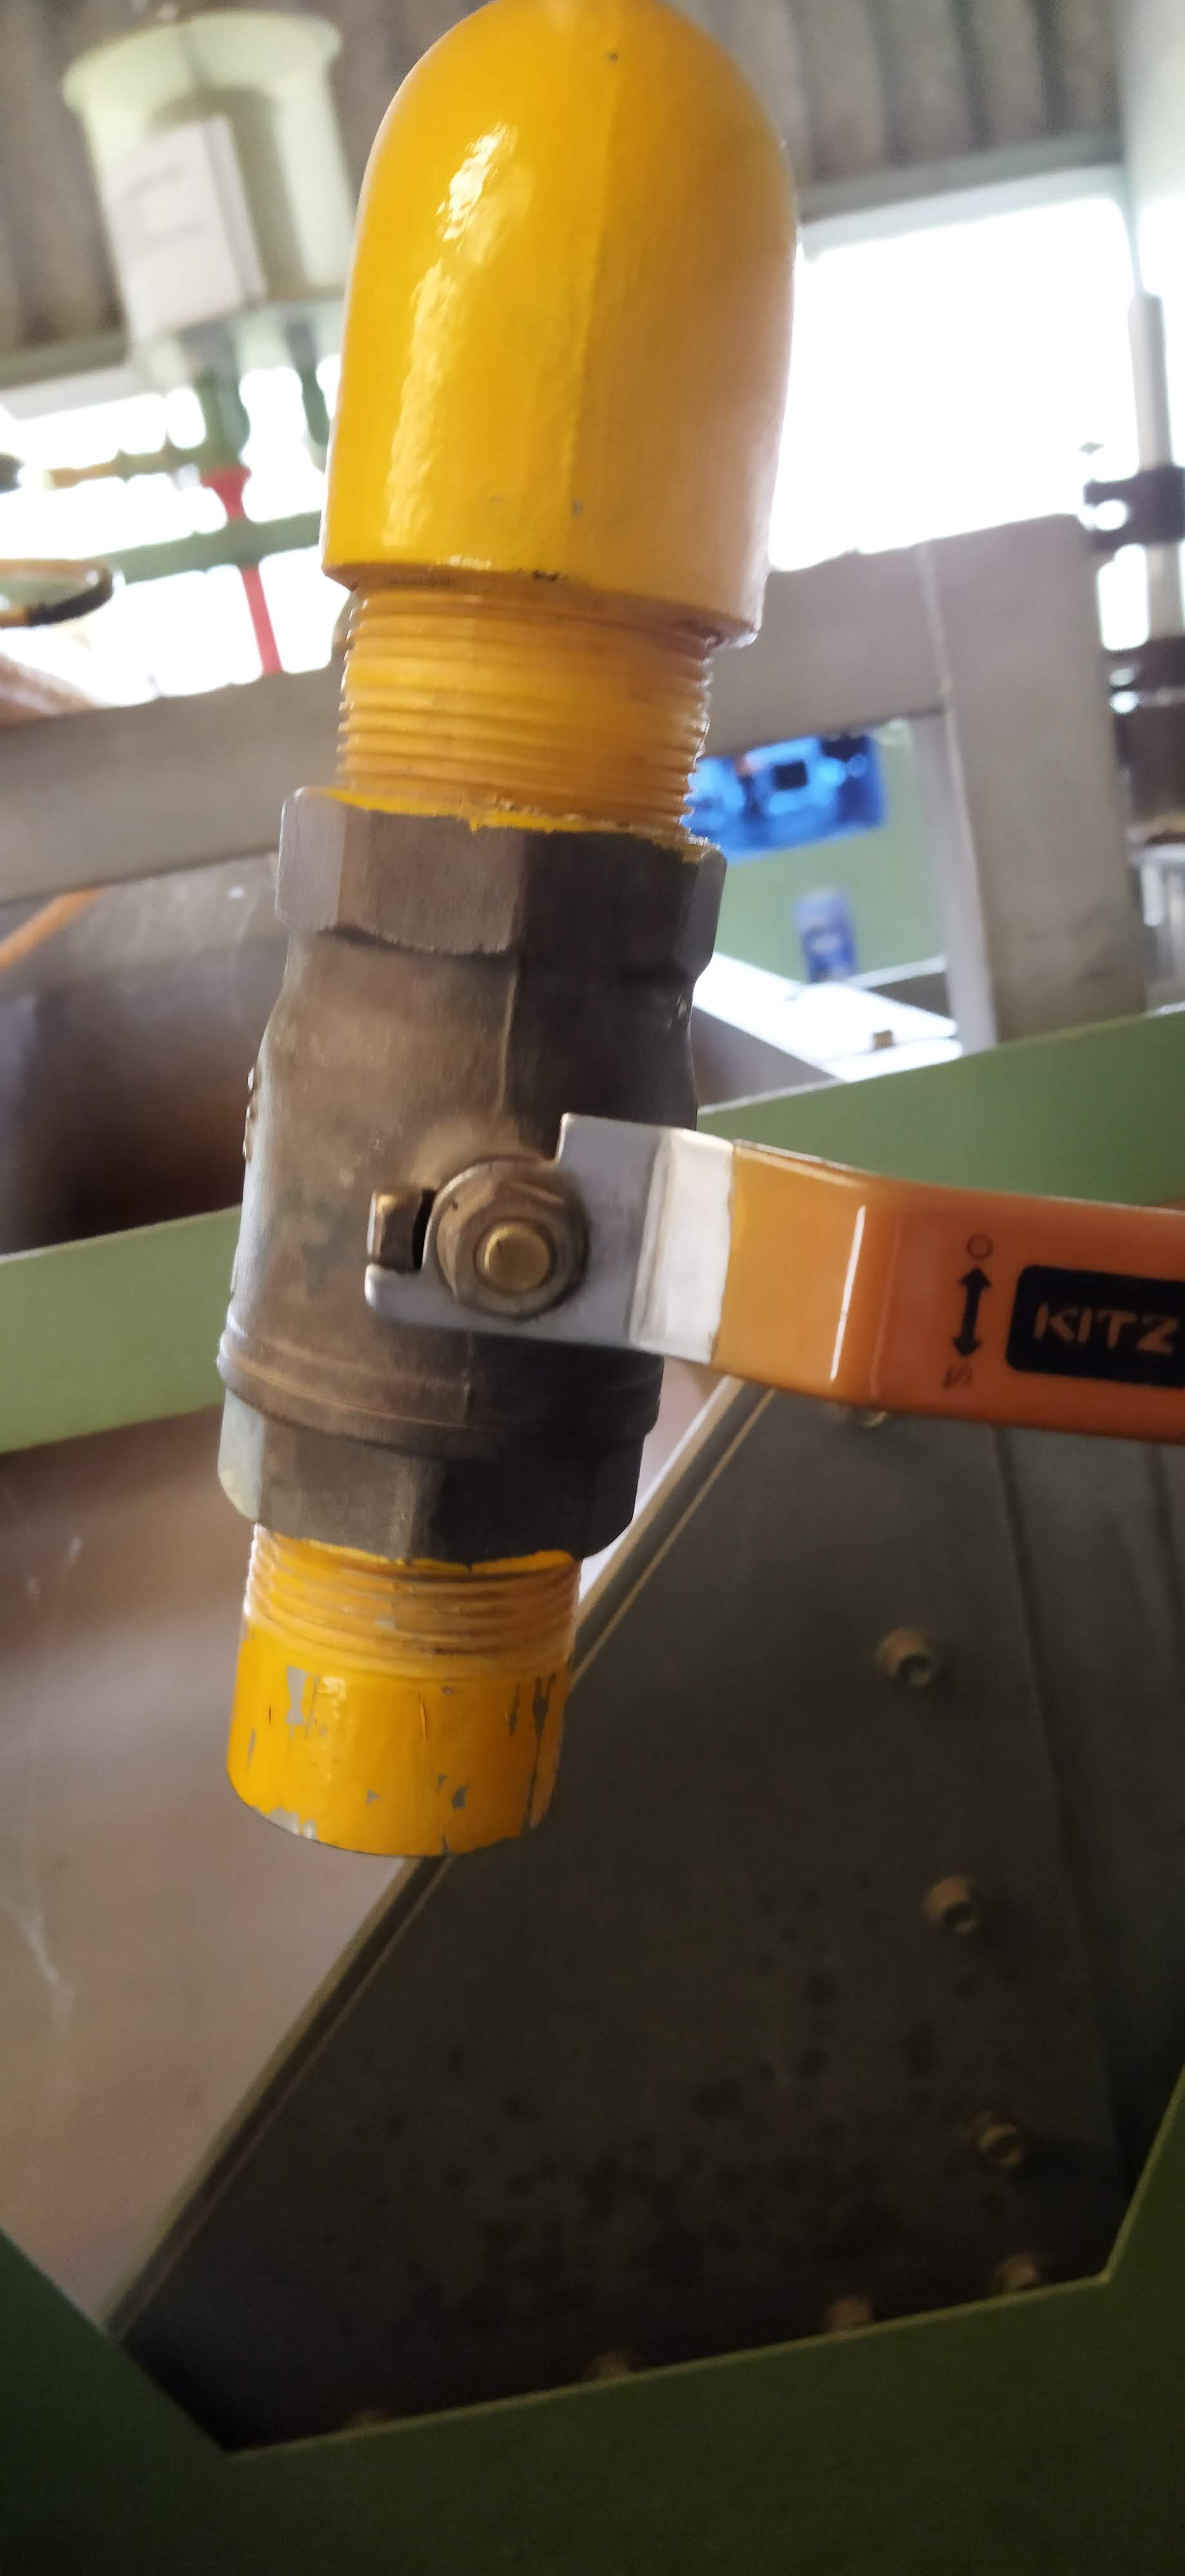
\includegraphics[height=0.25\textheight,keepaspectratio]{Figures/ballValve.jpg}
    \caption{Current discharge control unit}
    \label{fig:current_discharge_control_unit}
\end{figure}
\par
The $1 \frac{3}{4} inch $ ball valve on the main discharge pipe is opened in steps by hand using the lever. The size of a step is determined by human intuition.
\par
\textbf{Design}\\
To ensure minimum modification of the existing machine, the automation of this unit utilized the existing ball valve on the machine. The opening and closing of the valve is automated using a motorized system that can open the valve in precise steps.
\par
\textbf{Motor}
\par
The selection and the sizing of the motor for this application was based on the following considerations:

\begin{enumerate}
    \item The torque required to open and close the ball valve.
    \item The steps size 
\end{enumerate}
\par
Based on these two considerations, Servo and Stepper Motors were considered.
  \begin{table}[H]
    \centering
      \caption[Stepper versus Servo Motor]{Comparison between Stepper and Servo Motors \cite{nema17}\cite{mg996r}}
    \begin{tabular}{|m{5cm}|m{5cm}|m{5cm}|}
    \hline
  Difference & Servo Motor & Stepper Motor \\ \hline 
Operation &  Continuous &  Divided into discrete steps \\ \hline
Control system configuration & Closed loop control system & Open loop control system\\ \hline
Feedback mechanism & The feedback mechanism exists  &  No feedback mechanism \\ \hline
Torque speed characteristics &  High torque at high speeds &  High torque at low speeds \\ \hline
Hunting & Hunting exists during stop position &  No hunting during stop position \\ \hline
Efficiency & The efficiency of servo motor is comparatively high & The stepper motors are relatively less efficient  \\ \hline
Driver & Optional & Required \\ \hline
    \end{tabular}
    \label{tab:XLA_stuff}
    \end{table}
\begin{enumerate}
    \item \textbf{Stepper motor application}\\
    % This motor operates by accurately synchronizing position with the pulse signal output from the controller to the driver thus achieving highly accurate positioning and speed control. Stepper motors feature high torque and low vibration at low speeds ideally below 1500rpm, ideal for applications requiring quick fixed positioning in a short distance \cite{wargula2017investigations}. Furthermore, stepper motor rotates with a fixed step angle typically 1.8 degrees for a 2-phase. However, to achieve this requires the use of a micro-step driver.
    % \par
    % Besides having full control of rotation and speed, the simple structure of stepper motors is achieved without using electrical components, such as an encoder within the motor. For this reason, stepper motors are very robust and have high reliability with very few failures. As for stopping accuracy, ±0.05° (without cumulative pitch errors) is very accurate\cite{wargula2017investigations}. Because the positioning of stepper motors is performed by open-loop control, and operated by the magnetized stator and magnetic rotor with small teeth, stepper motors have a higher follow-up mechanism toward commands than the servo motors. Also, no hunting occurs when stopping it.
     \textbf{Design with stepper motor}
    \begin{enumerate}
    \item \textbf{Motor selection}\\
     Nema 17 Stepper motor shown in figure \ref{fig:Nema17 Steppper motor} was selected for this application. The motor can produce a $1.8^0$ step out of the box without a microstep driver. However, with the help of a microstep driver, it can produce as small as $1^0$ step.
    \begin{figure}[H]
        \centering
        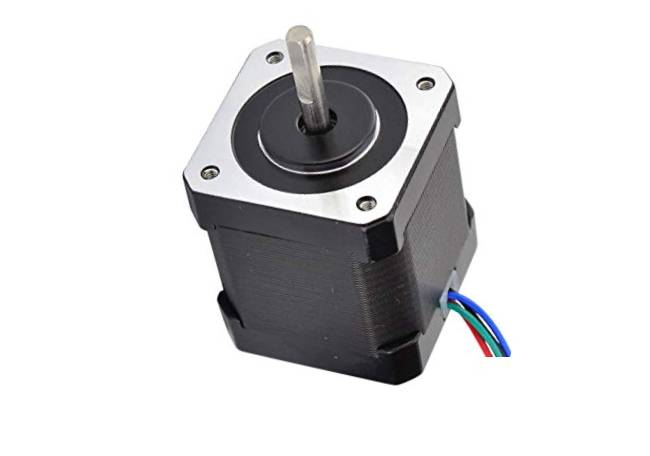
\includegraphics[width=.3\textwidth, height=.2\textheight]{Figures/Nema17Stepper.jpg}
        \caption[Nema 17 Stepper motor]{Nema 17 Stepper motor \cite{nema17}}
        \label{fig:Nema17 Steppper motor}
    \end{figure}
    \par
    Its technical specifications are as shown in the table \ref{tab:nema17_specs}:
\begin{longtable}{|l|l|}
\caption[Nema 17 Stepper Motor Technical specification]{Nema 17 Stepper Motor Technical specifications \cite{nema17}}
\label{tab:nema17_specs}\\
\hline
\textbf{Property} & \textbf{Value} \\ \hline
\endfirsthead
%
\multicolumn{2}{c}%
{{\bfseries Table \thetable\ continued from previous page}} \\
\hline
\textbf{Property} & \textbf{Value} \\ \hline
\endhead
%
Rated Voltage & 12V DC \\ \hline
Current & 1.2A at 4V \\ \hline
Step Angle & 1.8 deg \\ \hline
No. of Phases & 4 \\ \hline
Motor Length & 1.54 inches \\ \hline
4-wire, 8 inch lead &  \\ \hline
steps per revolution & 200 \\ \hline
Operating Temperature & -10 to 40 °C \\ \hline
Unipolar Holding Torque & 22.2 oz-in \\ \hline
Maximum torque & 4.8 Kg.cm \\ \hline
\end{longtable}

    \item \textbf{Ball valve - motor interface}
    \par
    An interface is required to connect the motor rotor to the ball valve. The following  two design options were considered for this application:
    \begin{itemize}
        \item An interface that could fit the rotor on one end and with claw-like configuration on the other end to turn the existing ball valve's lever.
        \item An interface that could fit the rotor on one end and with the other end, similar to the lever, that could be used in place of the lever.
    \end{itemize}
    \par
    The second option was chosen since the first choice will introduce a lag in a turn action since the point of action on the lever is displaced from the line of rotation of the rotor.
    \begin{figure}[H]
        \centering
        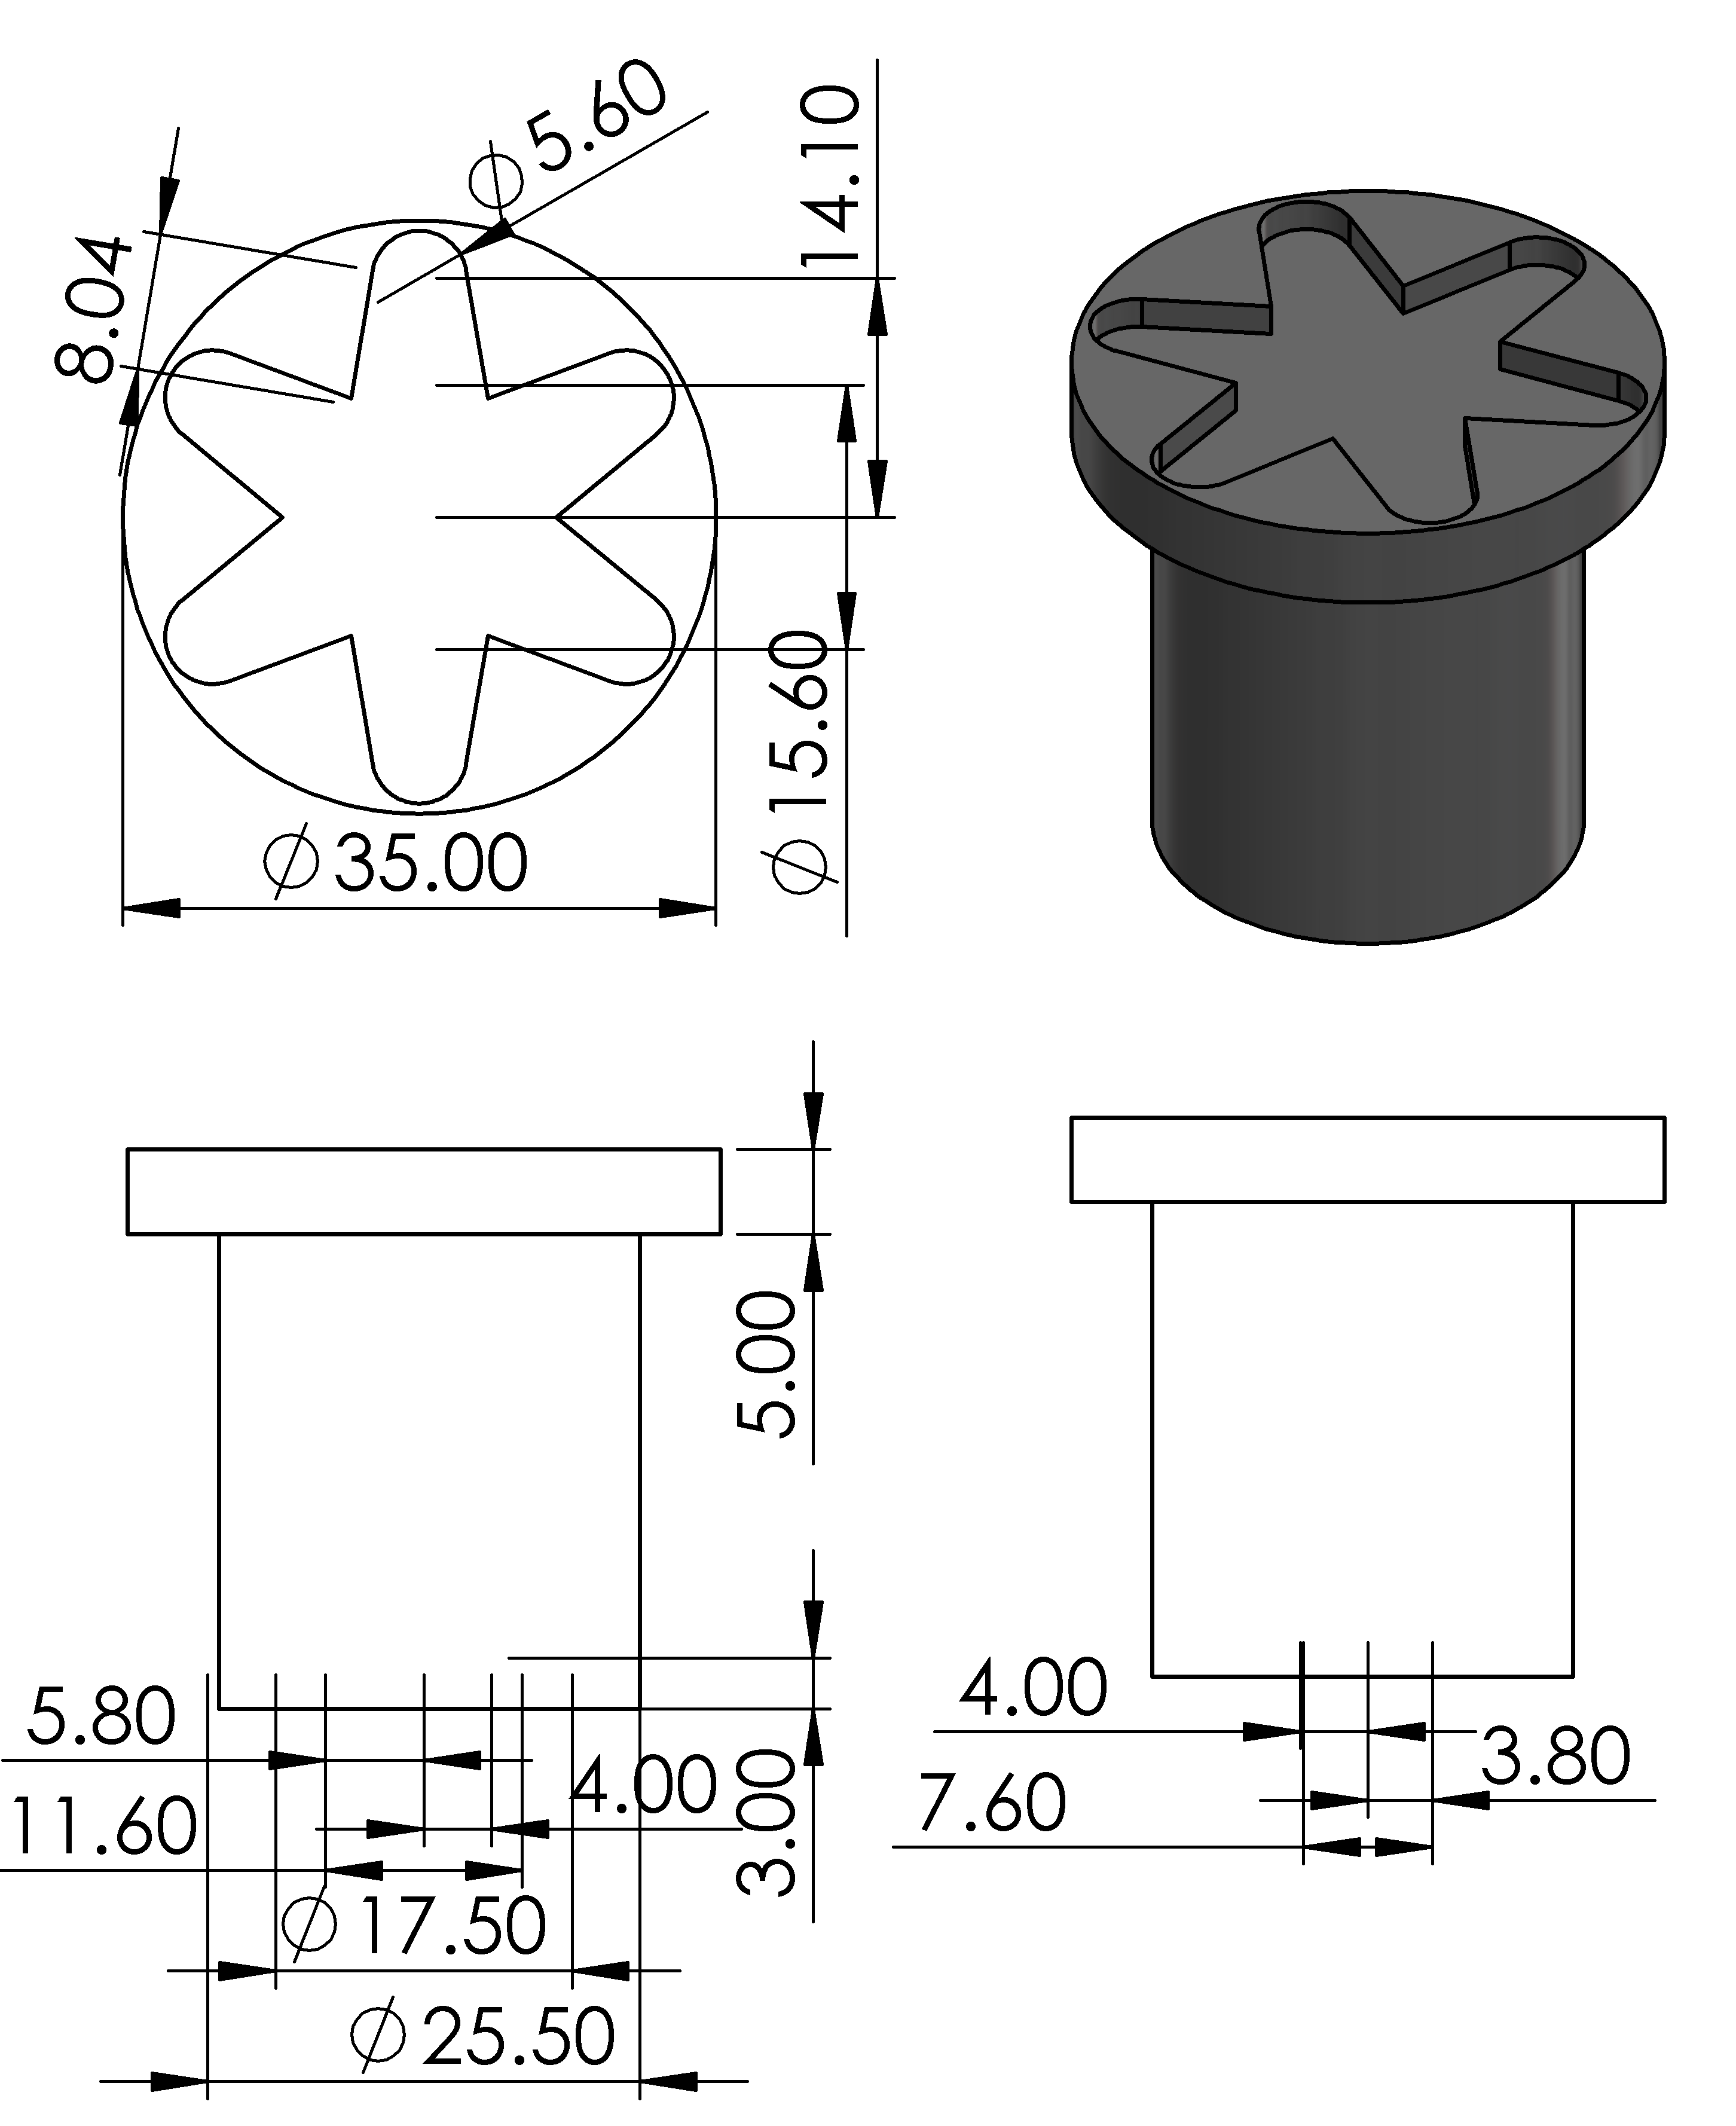
\includegraphics[height=0.5\textheight]{Figures/interface.PNG}
        \caption{Interface}
        \label{fig:Interface}
    \end{figure}
    Figure \ref{fig:Interface} shows the interface design. Dimensions of the interface, such as the width of its base, were measured and transferred from the existing lever currently on the machine.
    \par
    \item \textbf{Motor cage}
    \par
    The cage holds the motor in position on the ball valve as 
   shown in Figure \ref{fig:motor_cage_stepper}.
    
    \begin{figure}[H]
        \centering
        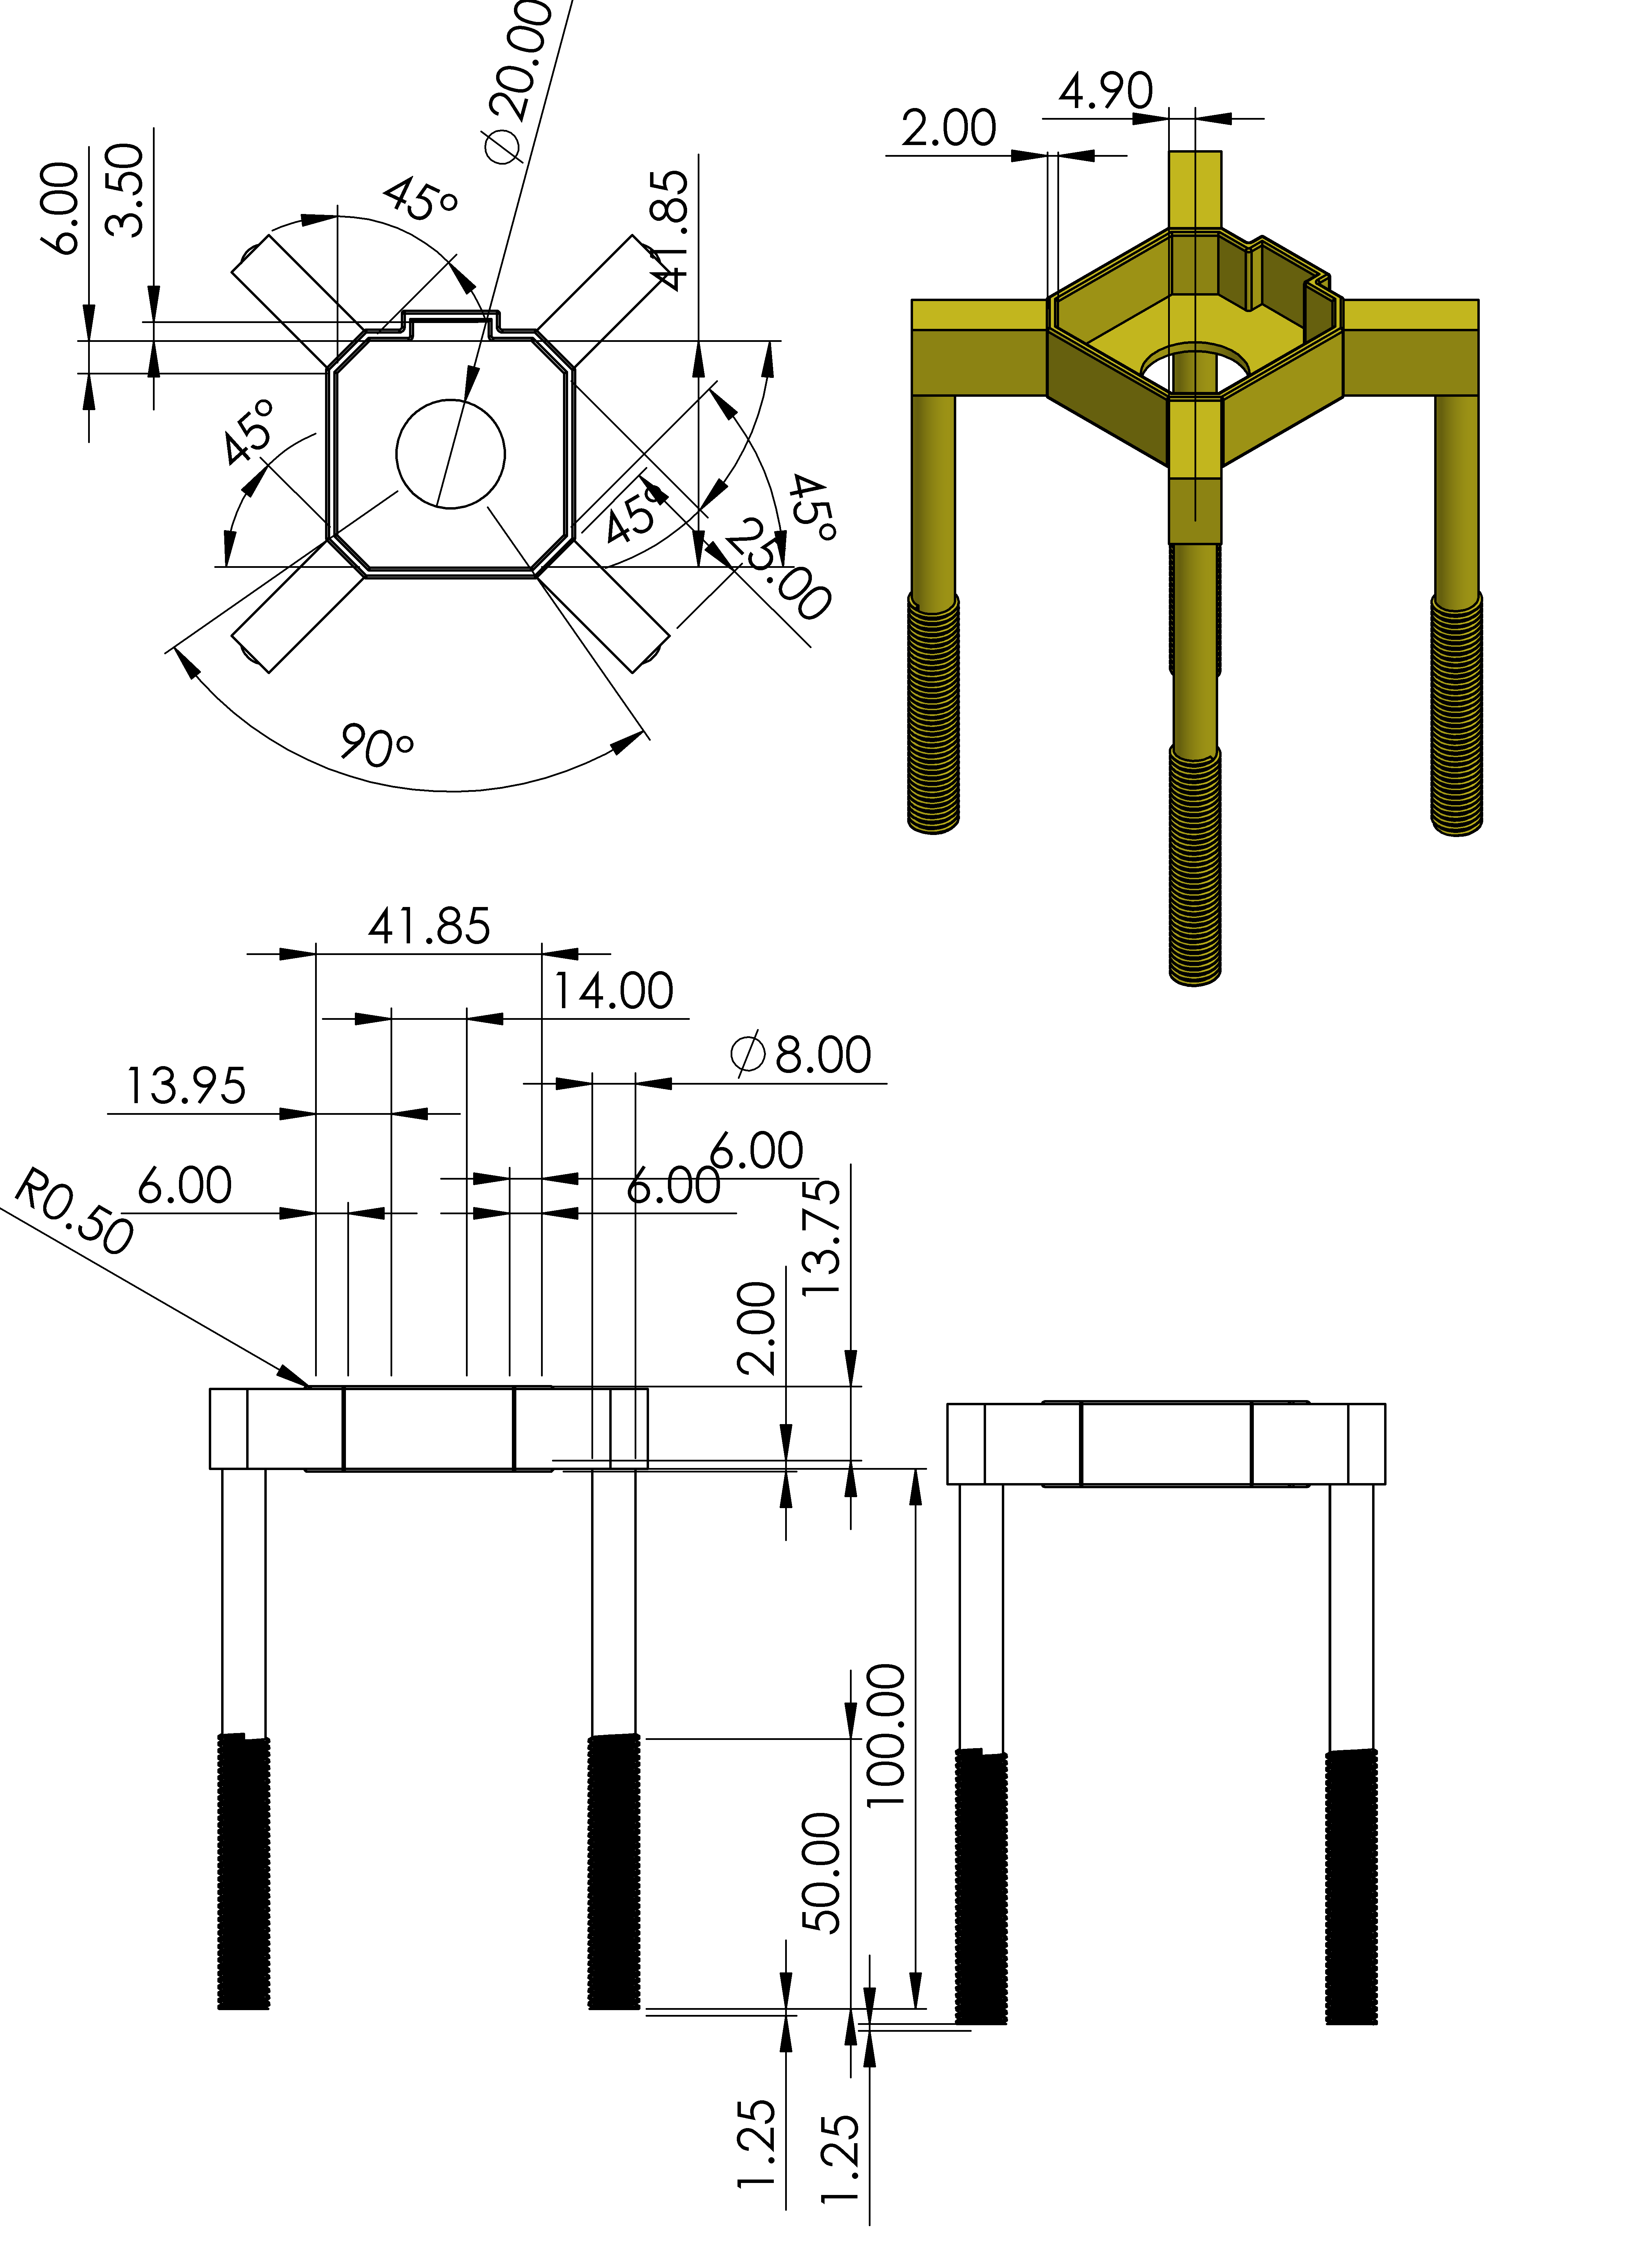
\includegraphics[height=.55\textheight]{Figures/MotorCage.PNG}
        \caption{Motor Cage}
        \label{fig:motor_cage_stepper}
    \end{figure}
    
    The dimensions of the cage in figure \ref{fig:motor_cage_stepper} were guided and determined from that of the stepper motor, the motor-ball valve interface, and that of the existing ball valve socket in order to accurately fit the socket.
    
    \item \textbf{Straps}
    \par
    It allows for the mounting of the cage onto the main discharge pipe as  shown in figure \ref{fig:mounting_straps_stepper}.
    
    \begin{figure}[H]
        \centering
        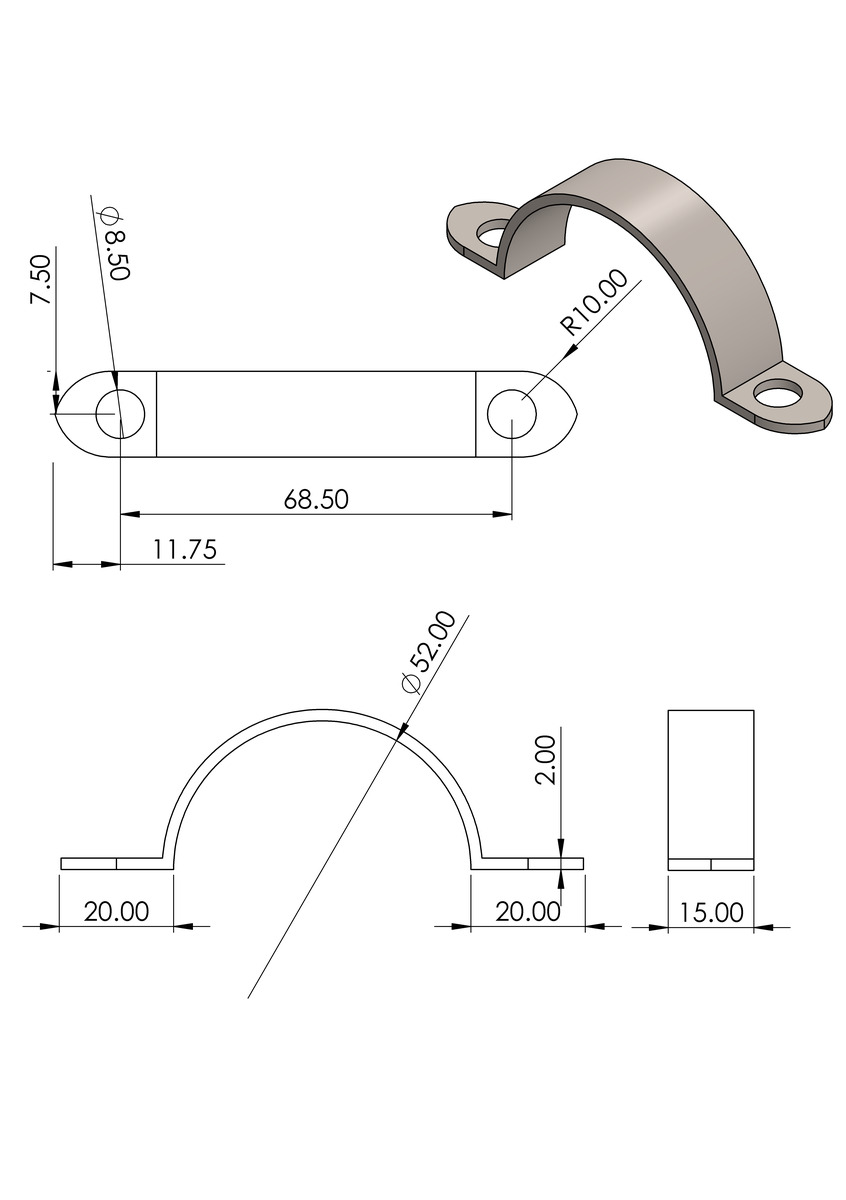
\includegraphics[height=.65\textheight]{Figures/strap.PNG}
        \caption{Mounting straps}
        \label{fig:mounting_straps_stepper}
    \end{figure}
 \item \textbf{Assembly of discharge flow control using stepper}
    \par
    The assembly of the discharge control unit is as shown in figure \ref{fig:stepper_actuated_ball_valve}. Nuts are used to fasten the whole structure on the main discharge pipe.
    
    \begin{figure}[H]
        \centering
        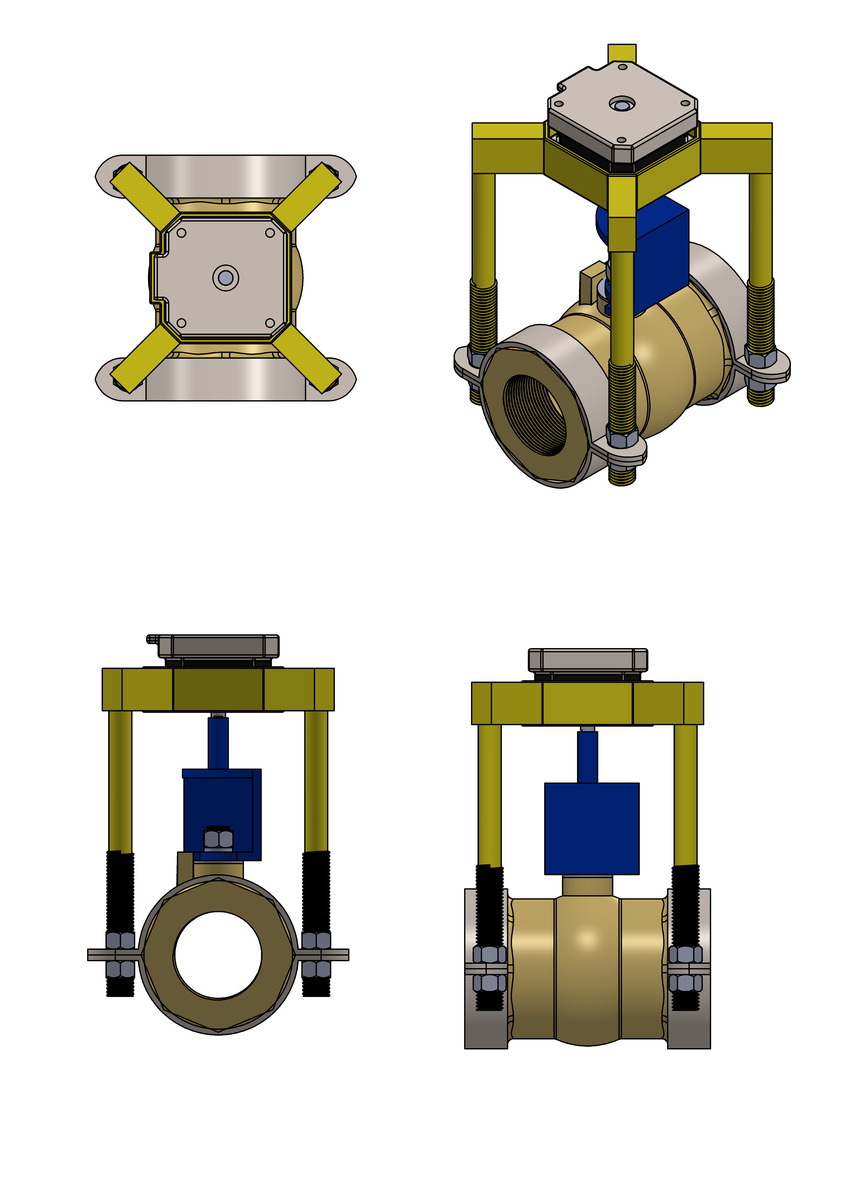
\includegraphics{Figures/ActuatedBallValve.PNG}
        \caption{Stepper Actuated ball valve}
        \label{fig:stepper_actuated_ball_valve}
    \end{figure}
    
    % \item \textbf{Finite element analysis of the assembly}
    % \par
    % The assembly was stress tested by applying a torque on the motor cage to determine if it could hold at the maximum torque of the motor. To do this, each part of this assembly was be assigned a material. Polyactic acid (PLA) was selected as the common material for all of the parts in the assembly. This is majorly due to the following reasons:
    % \begin{itemize}
    %     \item The maximum weight of the part to be supported by the structure is the stepper motor's weight, 450 grams. This can be supported by a 3D printed plastic support. A lighter material such as fiber glass or carbon fiber could be used but they are costlier than the set project's budget.
    %     \item The parts are complex for fabrication on the currently existing machinery in the university.
    % \end{itemize}
    % \item \textbf{Results}
    % \par
    % As shown in figure \ref{fig:SimulationResults}, the structure holds for the maximum torque of a Nema 17 stepper motor, $4.9 kg.cm$ or $0.4707192 Nm$.
    % \begin{figure}[H]
    %     \centering
    %     \includegraphics[width=\textwidth]{Figures/ActuatedBallValve-Static-1-1-1.png}
    %     \caption{Simulation results}
    %     \label{fig:SimulationResults}
    % \end{figure}
    
     
    \end{enumerate}
    
    
    \item \textbf{Servo motor application}\\
    % Servo motors run significantly faster than stepper motors, with speeds greater than 1500 rpm \cite{halicioglu2016mechanisms}. This enables servomotors to be used with gearboxes to deliver much higher torque at useful speeds. They also deliver more consistent torque across the speed range of the motor. Unlike stepper motors, they do not have holding torque. Closed-loop operation enables the controller/drive to command that the load remain at a specific position, however, and the motor will make continual adjustments to hold it there. Thus, servomotors can produce de facto holding torque\cite{halicioglu2016mechanisms}. The Servo motor rotates with a fixed step angle as low as 1 degree with or without the use of a driver. Furthermore, when powered, servomotors tend to move their shaft position to zero, a phenomenon known as hunting.
    \par
    \textbf{Design with servo motor}
    \begin{enumerate}
    \par
    \item \textbf{Motor selection}
    \par
    An MG996R Servo motor shown in figure \ref{fig:servo_motor_assembly} was selected for this application. It is the motor that provided the torque required to turn the ball valve at an optimum price for the project's budget. 
    \par
    The motor specification as shown in table \ref{tab:MG996R_servo_specs}.
    \begin{table}[H]
    \centering
    \caption[MG996R Servo motor specifications]{MG996R Servo motor specifications \cite{mg996r}}
    \begin{tabular}{|l|l|}
    \hline
    \textbf{Property} & \textbf{Value} \\ \hline
    Operating Voltage & +5V \\ \hline
    Current & 2.5A (6V) \\ \hline
    Stall Torque & 9.4 kg/cm (at 4.8V) \\ \hline
    Maximum Stall Torque & 11 kg/cm (6V) \\ \hline
    Operating speed & 0.17 s/60° \\ \hline
    Gear Type & Metal \\ \hline
    Rotation & 0°-180° \\ \hline
    Weight of motor & 55gm \\ \hline
    \end{tabular}
    \label{tab:MG996R_servo_specs}
    \end{table}
    \begin{figure}[H]
        \centering
        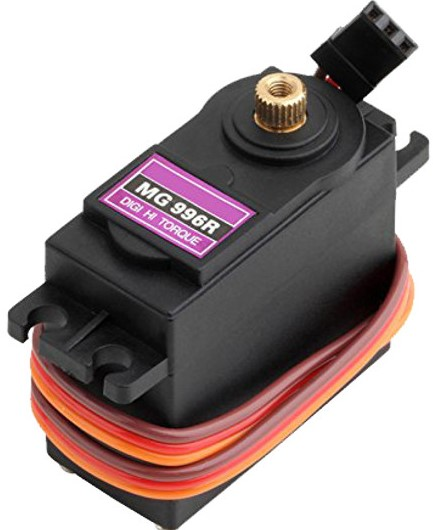
\includegraphics[width=.25\textwidth, height=.25\textheight]{Figures/MG996R.jpg}
        \caption[MG996R servo motor]{MG996R servo motor \cite{mg996r}}
        \label{fig:servo_motor_assembly}
    \end{figure}
    The servo motor homes to $0^{0}$ on powering hence the mounting mechanism should accommodate for this. Besides, the home position of the servo motor should be equal to the closed position of the ball valve. Therefore, during mounting, the servo motor must be rotated to align its home position with the closed position of the ball valve. Based on the above, the following considerations were made.
    % \par
    % The mounting mechanism should therefore allow for this rotation. A cuboid cage could have been used to support the motor in place, but since the centre of mass of this motor is displaced from its line of axle rotation, rotating the cuboid could mean repositioning the support stands for the cuboid.
    % \par
    %  There were two options that could achieve this kind of rotation:
     \begin{enumerate}
         \item A  cuboid cage with slots. The cuboid cage could hold the motor while the at the same time the slots provide for manual realignment.
         \par
         \textbf{Designs with this approach}
         \par
         \begin{itemize}
             \item \textbf{Servo motor cage}
            \par
            The cage shown in figure \ref{fig:servo_motor_cage} is screwed on to the motor straps. It just adds additional mounting points for the motor. 
            \begin{figure}[H]
                \centering
                \includegraphics[width=\textwidth]{Figures/MG996RHolder.PNG}
                \caption{Servo motor cage}
                \label{fig:servo_motor_cage}
            \end{figure}
            \par
            % \item \textbf{Mounting plate}
            % \par
            % Figure \ref{fig:servo_motor_mounting_plate} shows the mounting plate for the motor cage. The plate is like a ring with slots. The design allows for rotation without the need to reposition the supporting rods. 
            % \par
            % \begin{figure}[H]
            %     \centering
            %     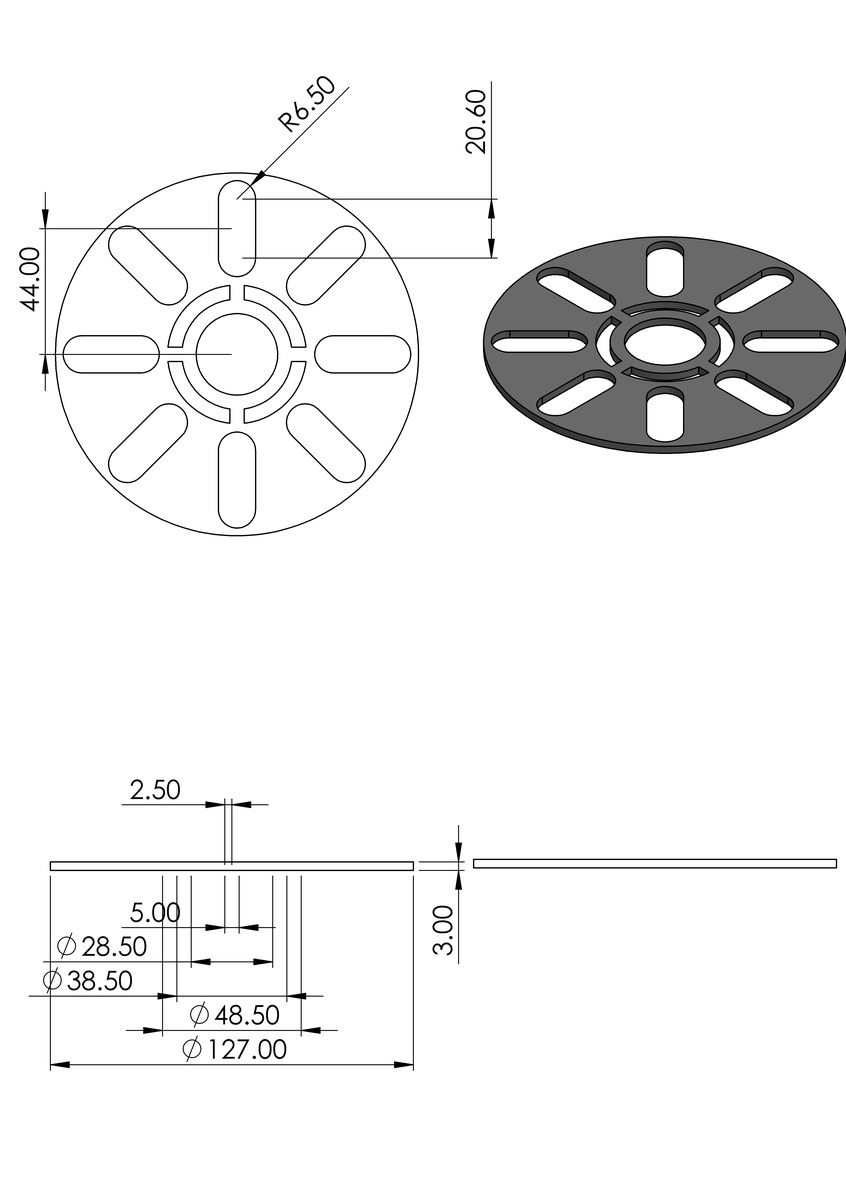
\includegraphics[height=.7\textheight]{Figures/ServoMotorHolderMount.PNG}
            %     \caption{Servo motor mounting plate}
            %     \label{fig:servo_motor_mounting_plate}
            % \end{figure}
            \par
            \item \textbf{The holder assembly}
            \par
            Figure \ref{fig:servo_motor_mounted_assembly} shows the servo motor cage with the servo motor mounted on the mounting plate. The servo motor assembly can be rotated and translated to reposition the line of rotation of the motor axle. 
            \begin{figure}[H]
                \centering
                \includegraphics[height=.5\textheight, width=.6\textwidth]{Figures/MG996RServoMounted.PNG}
                \caption{Servo motor mounted assembly}
                \label{fig:servo_motor_mounted_assembly}
            \end{figure}
             This design can allow for both rotational and translational adjustments along the slots. However, it is complex and require a lot of fasteners.
         \end{itemize}
         \item A combination of spur gears to always translate the line of rotation of the motor axle to a fixed line of rotation no matter the orientation of the motor.
         \clearpage
         \textbf{Designs with the spur gears approach}
         \par
          \begin{itemize}
              \item \textbf{Spur gears}
              \par
              Spur gear shown in Figure \ref{fig:spur_gear} translates the line of rotation by 5.75mm in any orientation of the servo to a fixed centre line.
              \begin{figure}[H]
                  \centering
                  \includegraphics[height=.55\textheight]{Figures/SpurGear1.PNG}
                  \caption{Spur gear}
                  \label{fig:spur_gear}
              \end{figure}
              \par 
              \item  \textbf{Servo motor-spur gear assembly}
              \par
              Figure \ref{fig:servo_motor_with_spur_gears} shows the spur gear translation system assembled with the servo motor.
              \begin{figure}[H]
                  \centering
                  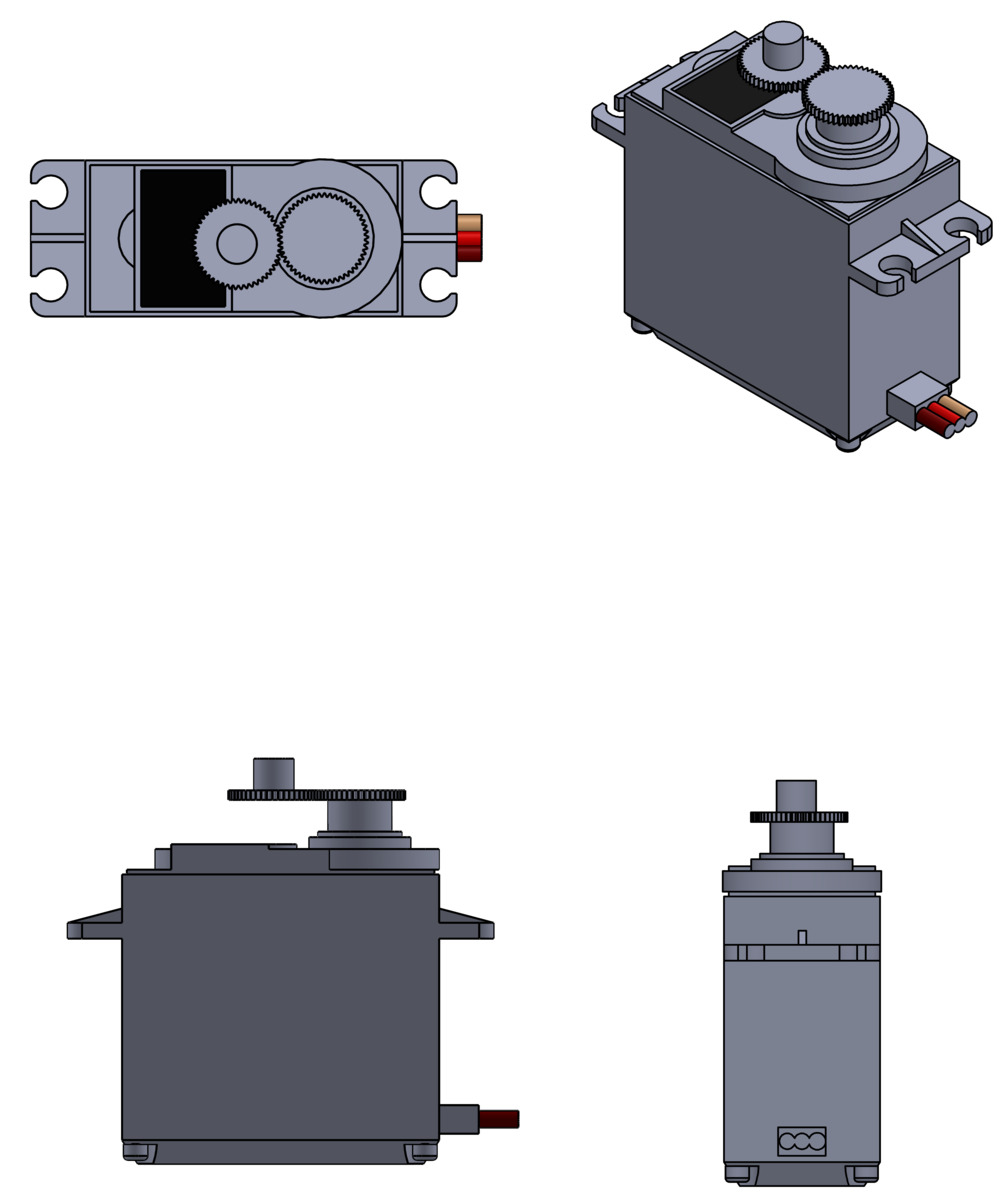
\includegraphics[height=.55\textheight]{Figures/ServoMotorWithSpurGears.PNG}
                  \caption{Servo motor with spur gears}
                  \label{fig:servo_motor_with_spur_gears}
              \end{figure}
              This design is quite simpler than the first approach. The design considerations are few and can produce even finer translations in the scale of the spur gear pitch($1 mm$). However, the main challenge with this design is the durability of spur gears made of PLA material since servo motors tend to have a high starting torque. This will almost necessitate the replacement of the gears after every two or three experiments.  
          \end{itemize}
     \end{enumerate}
     \par
     The cuboid cage was selected as it requires little maintenance as with the case of spur gears due to wear and tear.
    %  Between the two mounting designs described, the first options had more merits than the second option. It might require more material to produce it but at least it is only for one time unlike with second option where the gears are to be replaced after every two or three times in operation.
     \par 
     \item \textbf{Mounting rod}
     \par
     Two of the rod shown in figure \ref{fig:mounting_rods} are used to support the mounted servo motor assembly on the ball valve. The design was such that it allowed for fasteners on both sides: at one end, to fasten the servo motor assembly after alignment and at the other end, to fasten the whole flow control unit on the main discharge pipe. The protrusion of its surface eliminates the need for another fastener. 
      \begin{figure}[H]
          \centering
          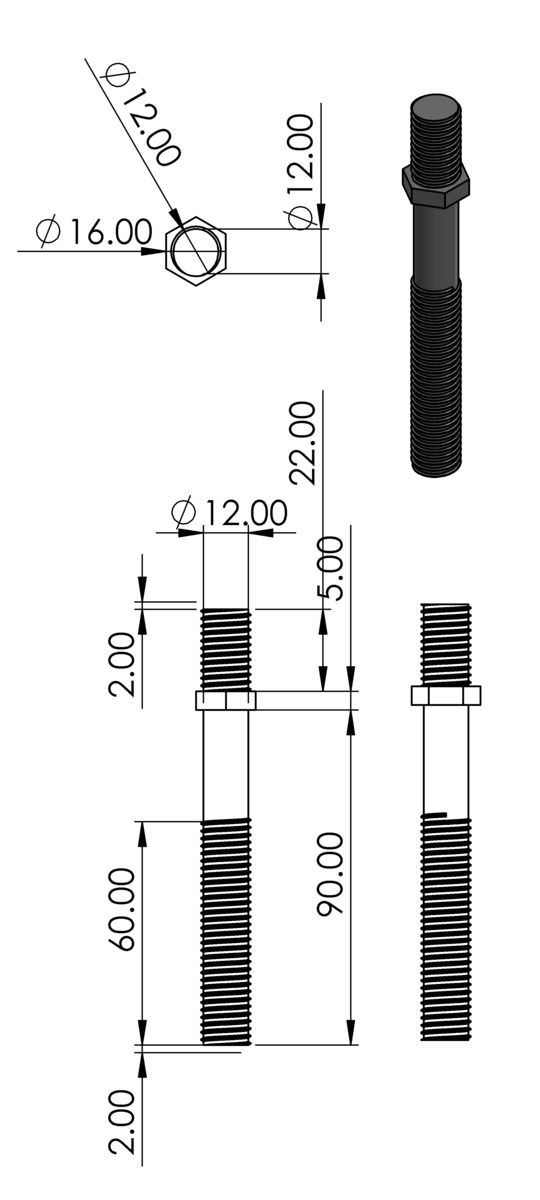
\includegraphics[height=.55\textheight]{Figures/ServoMotorMountRods.PNG}
          \caption{Mounting rods}
          \label{fig:mounting_rods}
      \end{figure}
      \par
    \item \textbf{Interface}
    \par
    The interface shown in Figure \ref{fig:interface2} is an improvement from the interface that was used with the stepper motor. This design is minimalistic and requires a lesser volume of material to produce. 
    \begin{figure}[H]
        \centering
        \includegraphics[height=.5\textheight]{Figures/Interface.PNG}
        \caption{Interface}
        \label{fig:interface2}
    \end{figure}
    \par
    \item \textbf{Straps}
    \par
    Serrated straps shown in \ref{fig:two_rail_serrated_straps} are also an improvement on the straps used in the stepper motor approach. The serration provide more grip on the discharge pipe.The sizing and dimensioning was guided by the existing ball valve casing.
    \begin{figure}[H]
        \centering
        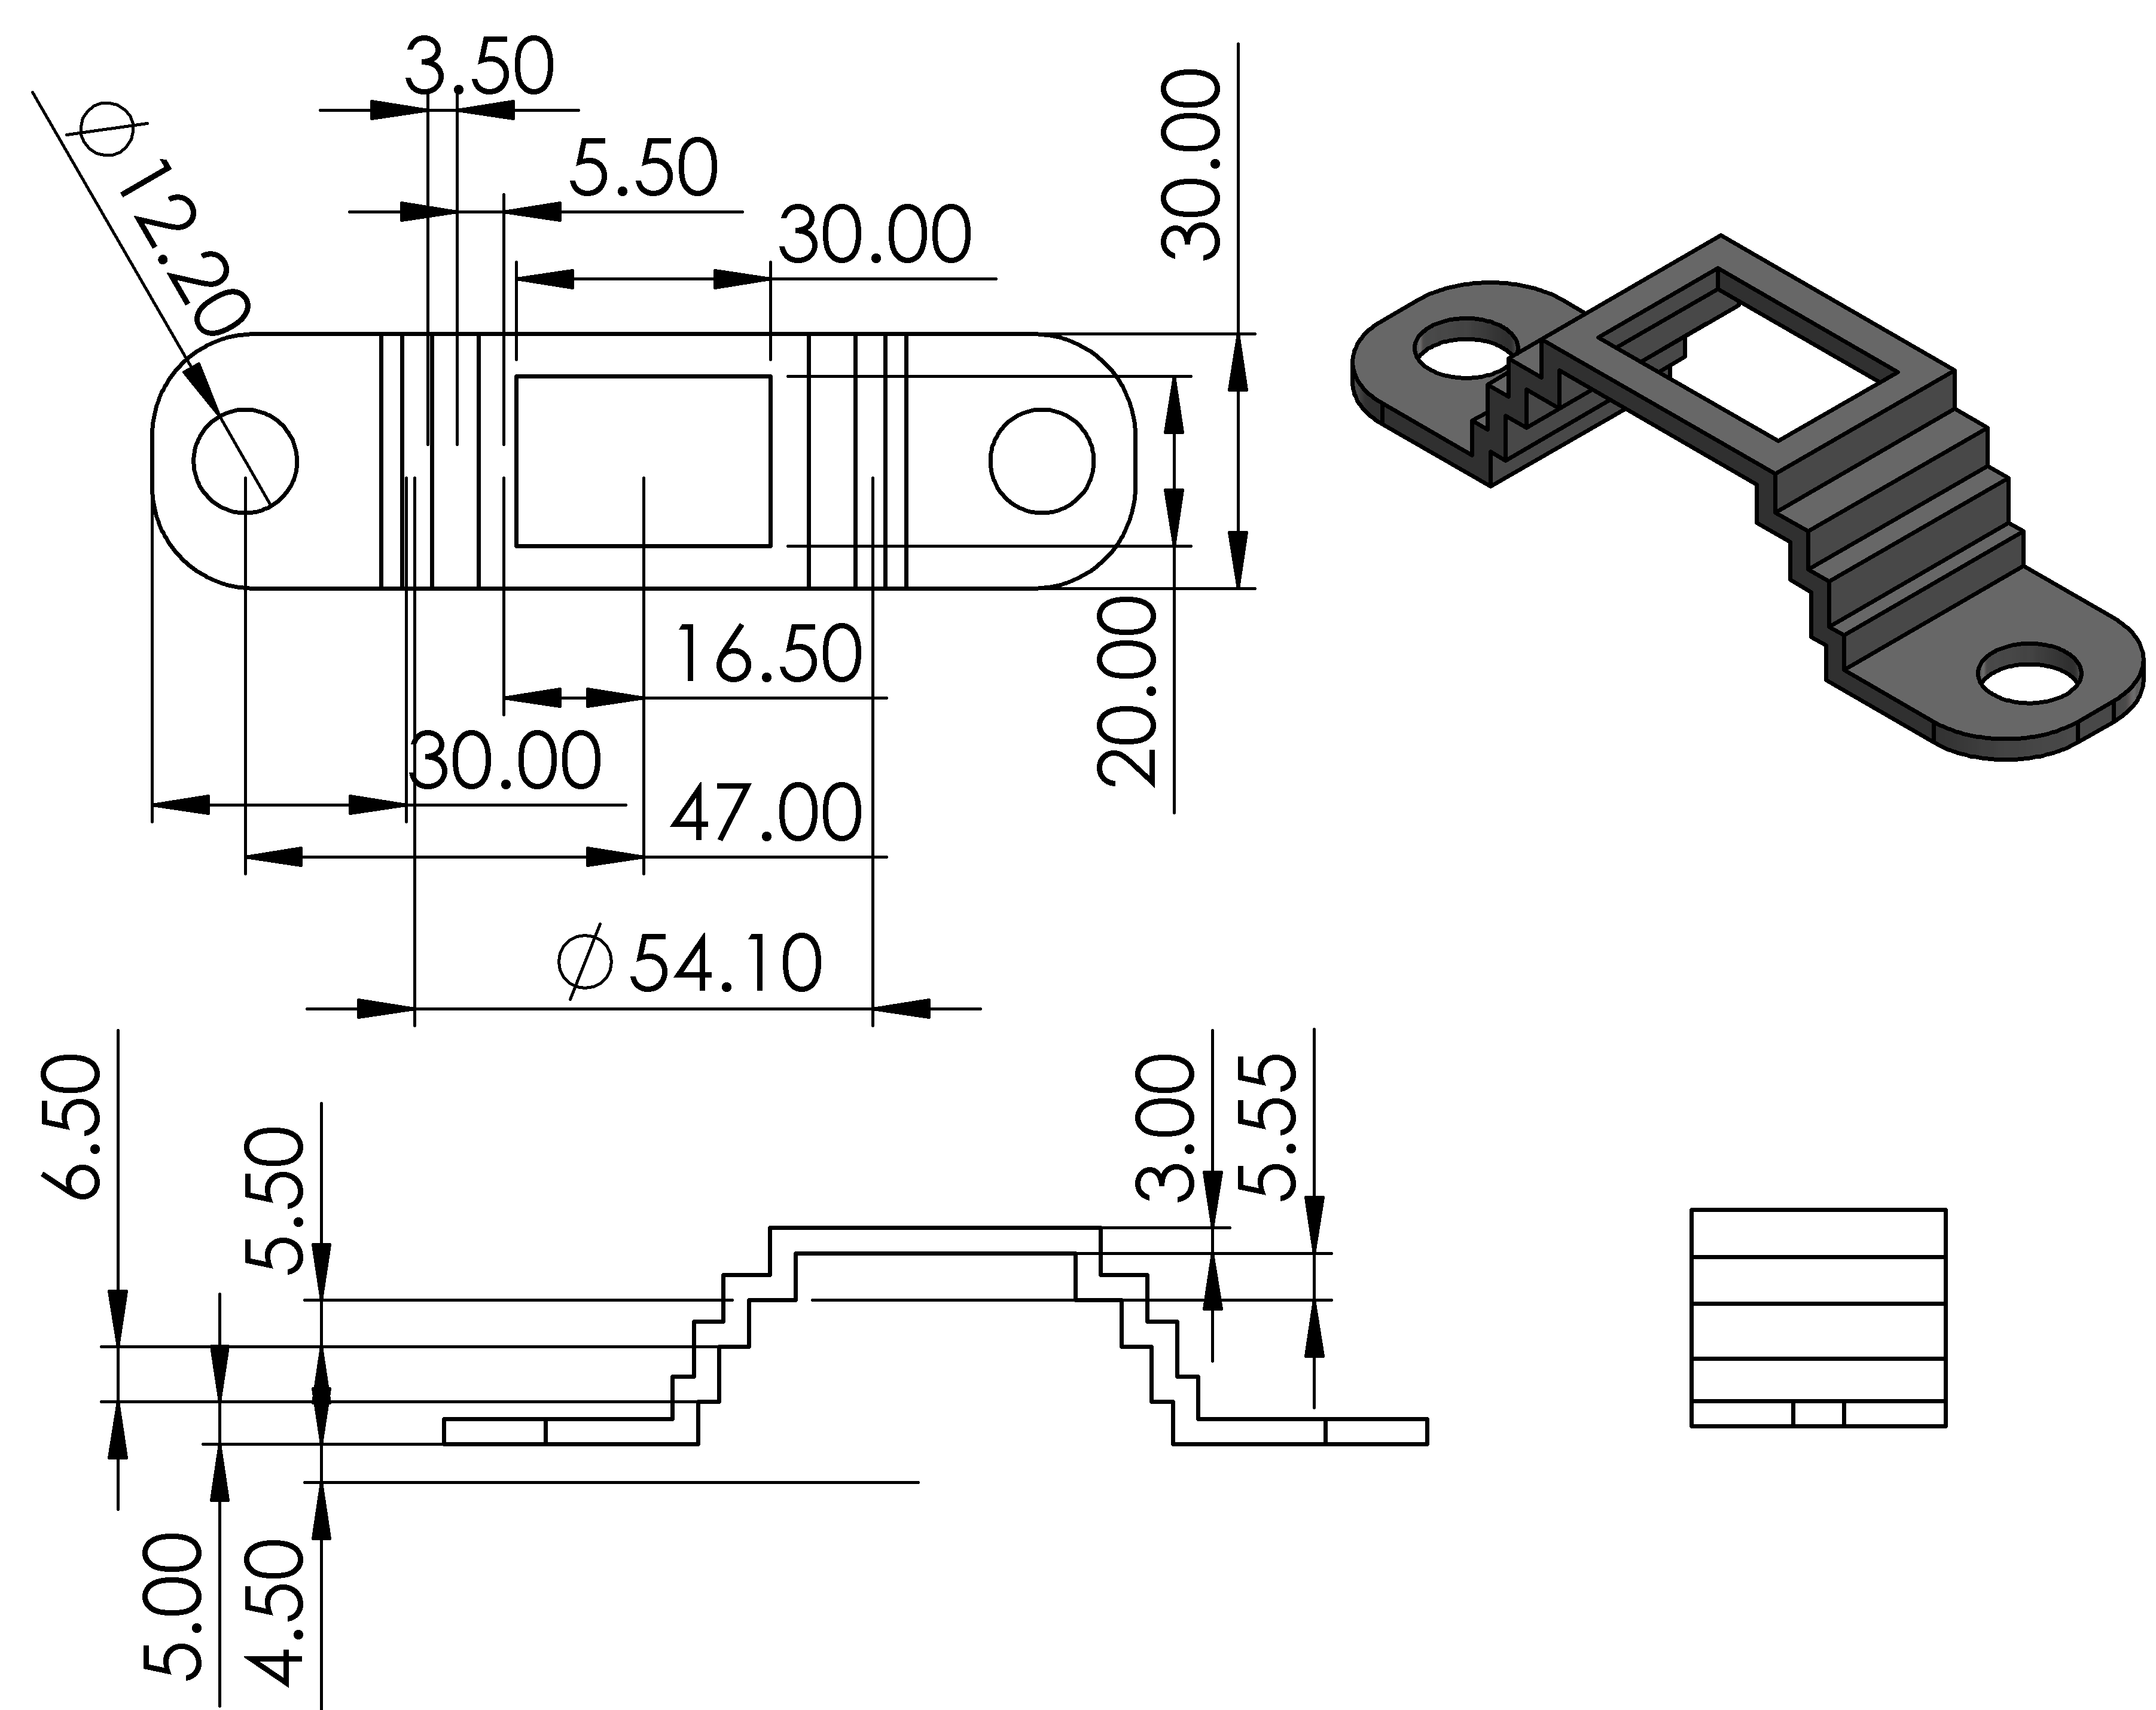
\includegraphics[height=.45\textheight]{Figures/twoRailStrapsTop.PNG}
        \caption{Top strap}
        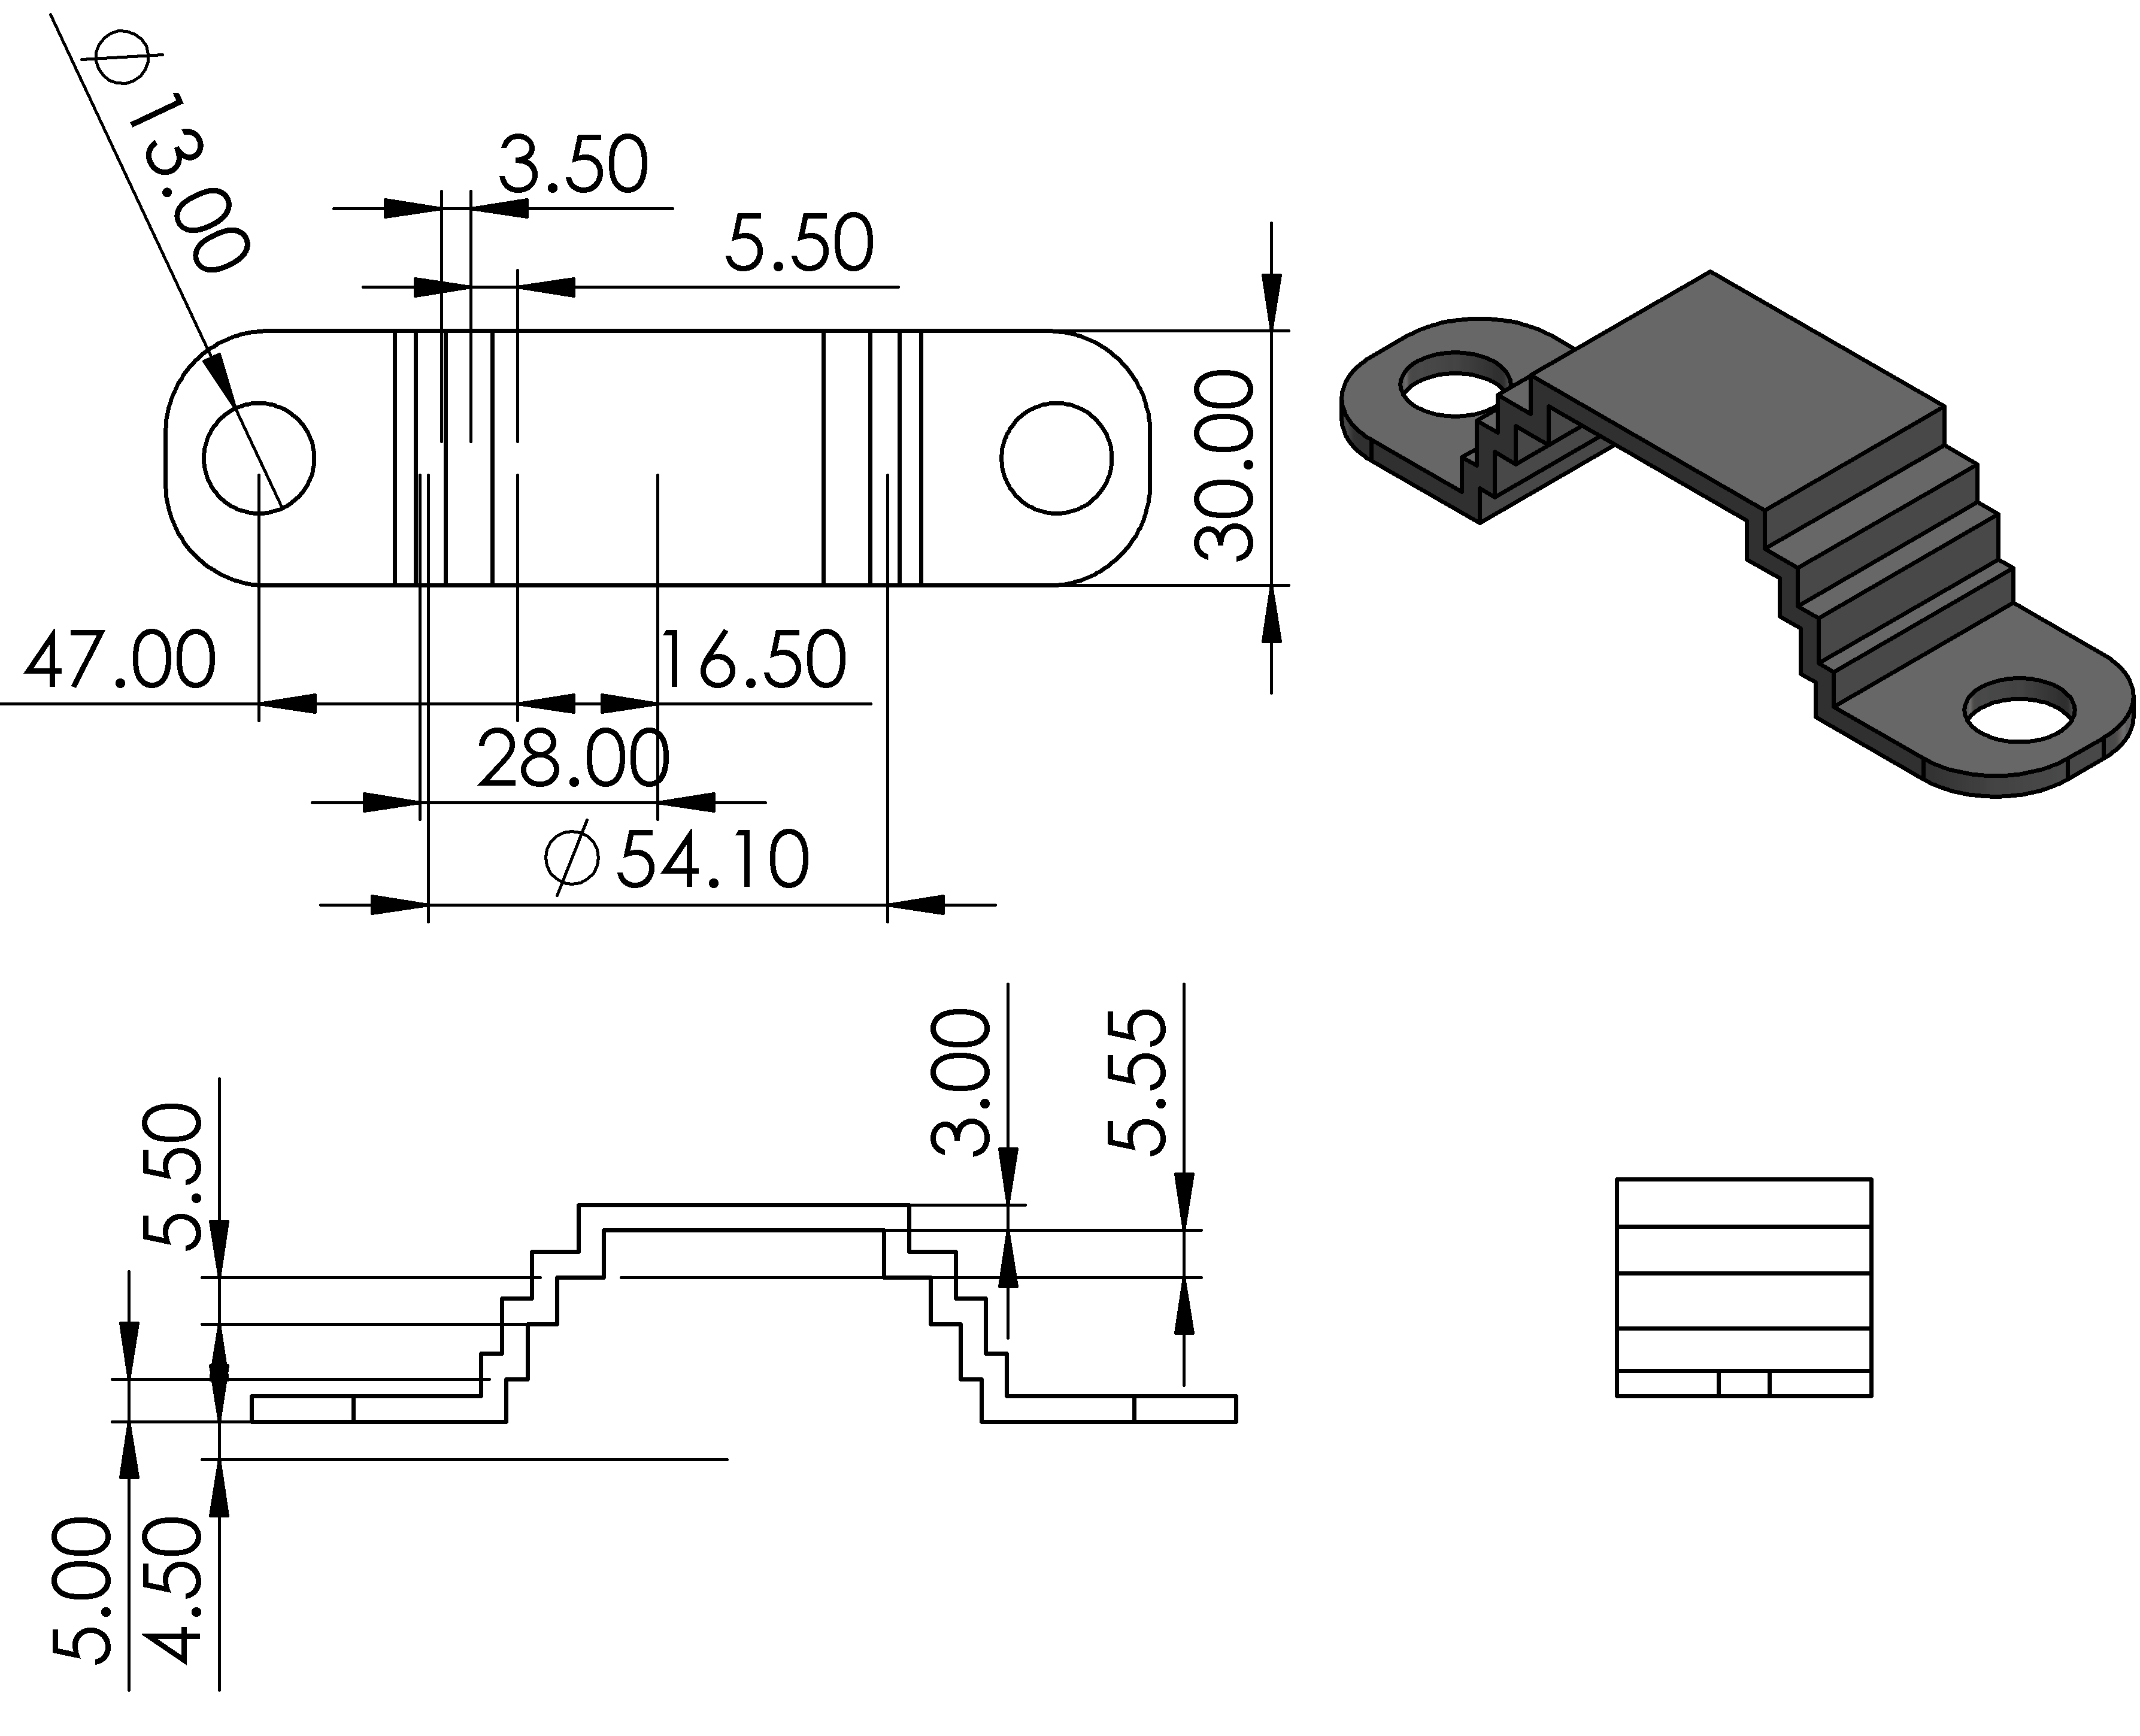
\includegraphics[height=.45\textheight]{Figures/twoRailStrapsBottom.PNG}
        \caption{Bottom strap}
        \label{fig:two_rail_serrated_straps}
    \end{figure}
      
    \par
    \item \textbf{Servo motor discharge flow control assembly}
    \par
    The assembly of parts used in the servo motor approach is as shown in Figure \ref{fig:servo_motor_discharge flow control assembly}.
     \begin{figure}[H]
         \centering
         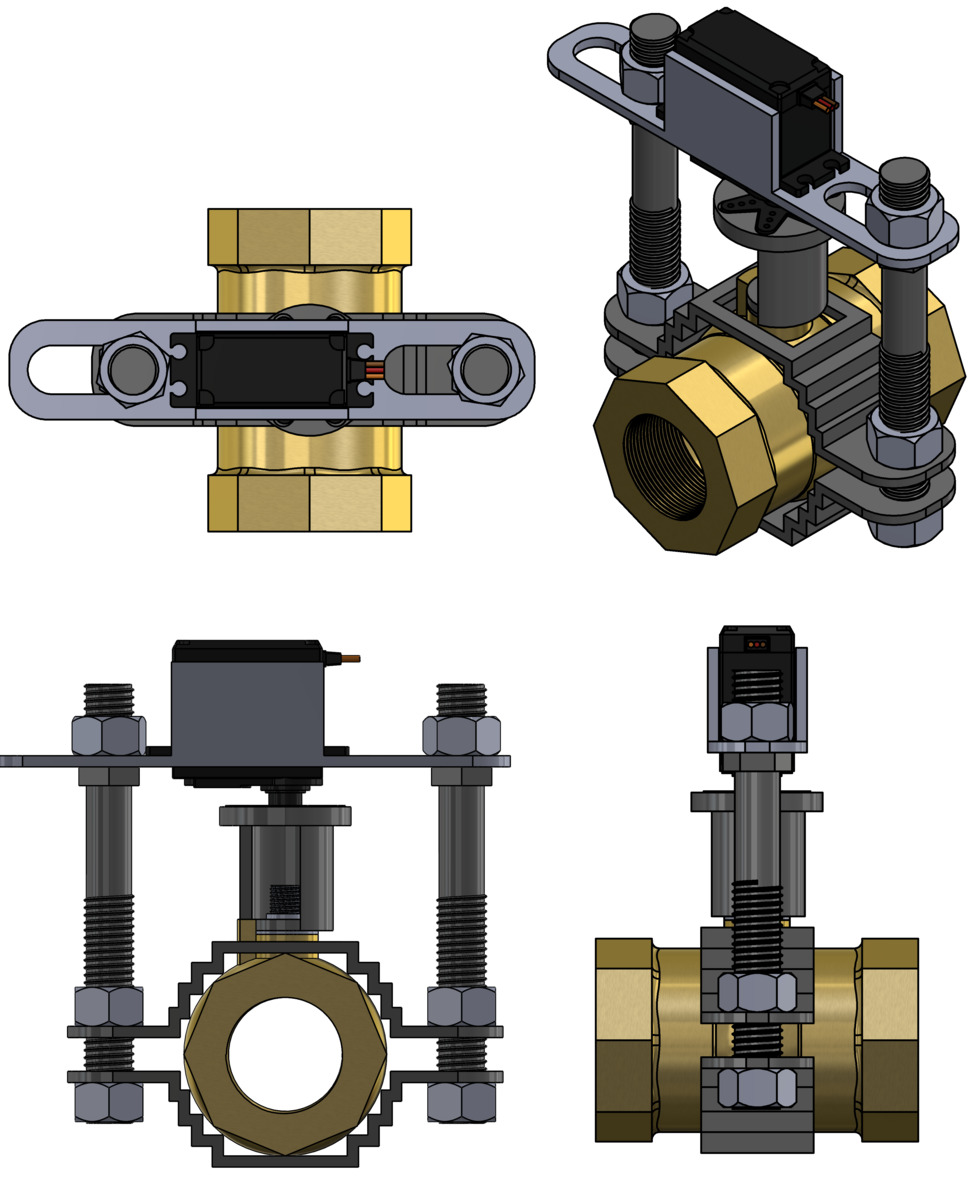
\includegraphics[height=.55\textheight]{Figures/FlowControlSubUnitAssembly.PNG}
         \caption{Servo motor discharge flow control assembly}
         \label{fig:servo_motor_discharge flow control assembly}
     \end{figure}
      
    %  \par
    %  \item \textbf{Finite element analysis of the assembly}
    %  \par
    %  PLA material was assigned to each part of the structure. The maximum load torque of the servo motor($11kg.cm$) was then applied on the mounting plate of the motor. The results of the simulation were as shown in figure \ref{fig:servo_assembly_results}. From the results, the structure still holds to the maximum torque with minimal displacement.
    %  \begin{figure}[H]
    %      \centering
    %      \includegraphics[width=\textwidth]{Figures/ServoHolderBallValveAssembly-Static-1-1-1.png}
    %      \caption{Servo Assembly simulation results}
    %      \label{fig:servo_assembly_results}
    %  \end{figure}
    \end{enumerate}
\end{enumerate}

From these two design approaches, the servo motor approach was selected.

\subsubsection{Flow diversion sub-unit}
The design of this unit was based on the following two considerations:
\begin{enumerate}
    \item A faster response time. It is the time it takes to divert the discharge flow into the main reservoir or the discharge collection tank. 
    \item An actuator that can provide linear translation of not less than 30 mm. In fact the longer the better. This is measured from the design assembly. This ensures that the discharge is fully diverted into the collection tank or to the main reservoir. 
\end{enumerate}

Based on the above two considerations, the use Piezo-electric actuato and Electromagnetic Actuator were feasible options. 
\begin{table}[H]
    \centering
      \caption[Piezo-electric actuator versus Electromagnetic Actuator]{Comparison between Piezo-electric actuator and Electromagnetic Actuator \cite{xla3} \cite{la_t8}}
    \begin{tabular}{|m{3cm}|m{5cm}|m{5cm}|}
    \hline
Parameters & Piezo-electric actuator & Electromagnetic Actuatorr \\ \hline 
Displacements & Small mechanical displacements at high speed & Large mechanical displacements \\ \hline
Precision&High precision positioning & Low precision positioning\\ \hline
Force & Large generated force & Relatively large force generated\\ \hline
    \end{tabular}
\end{table}
\begin{enumerate}
    \item \textbf{Piezo-electric actuator}
    \par
      Xeryon Precision XLA-Series 3 piezo actuator shown in Figure \ref{fig:piezo_actuator} was selected since it satisfied all the design requirements required for this subunit.
    \begin{figure}[H]
        \centering
        \includegraphics{Figures/Xeryon-XLA-3-1.png}
        \caption[Xeryon-XLA Series 3 piezo actuator]{Xeryon-XLA Series 3 piezo actuator \cite{xla3}}
        \label{fig:piezo_actuator}
    \end{figure}
    Its technical specifications are as shown in table \ref{tab:XLA_stuff}.
    \begin{table}[H]
    \centering
      \caption[XLA series 3 piezo actuator specifications]{XLA series 3 piezo actuator specifications \cite{xla3}}
    \begin{tabular}{|l|l|}
    \hline
    \textbf{Property} & \textbf{Value} \\ \hline
    Stroke Length & 45mm \\ \hline
    Resolution & 312nm \\ \hline
    Operating voltage & 20-48V \\ \hline
    Control & Closed loop control with an external XD-A controller \\ \hline
    Temperature & -30  to 70 \\ \hline
    Holding\& Driving  force & 3N \\ \hline
    Speed range & 2mm / s to 400mm / s \\ \hline
    \end{tabular}
    \label{tab:XLA_stuff}
    \end{table}
    
    
    From the technical specifications in the table, it is evident that this actuator could be the best choice for this application. However, it requires an external proprietary controller for closed-loop control. Xeryon company products are also not available in public stores such as Amazon or Aliexpress.
    
    \item \textbf{Electromagnetic Actuator}
    \par
    Electromagnetic actuators work on the principle of electromagnetism where electrical energy is converted to a linear translational mechanical motion and vice versa.
    \par
     LA-T8 micro linear actuator shown in figure \ref{fig:la_t8_linear_actuator}  was selected for this application.
    \begin{figure}[H]
        \centering
        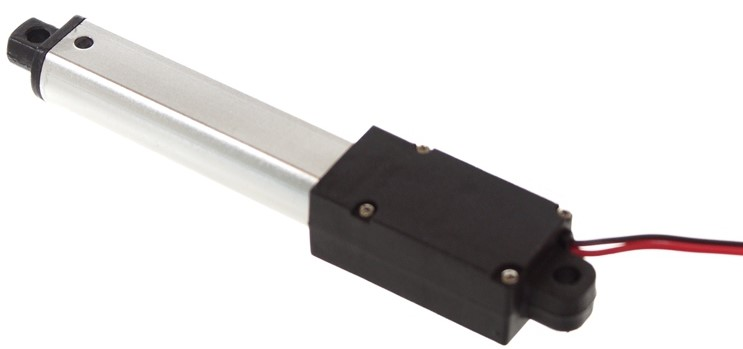
\includegraphics[width=.25\textwidth, height=.25\textheight]{Figures/LA-T8.jpg}
        \caption[LA-T8 linear actuator]{LA-T8 linear actuator \cite{la_t8}}
        \label{fig:la_t8_linear_actuator}
    \end{figure}
    % Its technical specifications are shown in table \ref{tab:la_t8_tab}.
    \begin{table}[H]
    \centering
       \caption[LA-T8 Micro-linear actuator technical specifications]{LA-T8 Micro-linear actuator technical specifications \cite{la_t8}}
    \begin{tabular}{|l|l|}
    \hline
    \textbf{Property} & \textbf{Value} \\ \hline
    Operating voltage & 12V DC \\ \hline
    Stroke length & 100mm \\ \hline
    Stroke speed & 150mm/s \\ \hline
    Maximum load & 6.4N \\ \hline
    \end{tabular}
    
    \label{tab:la_t8_tab}
    \end{table}
    The actuator satisfies optimally the requirements required for this application. However, unlike the piezo actuator, this device is available and for a cheaper price.
\end{enumerate}
Based on the above descriptions, the LA-T8 micro-linear actuator was selected for this application. This because of its local availability and the large mechanical displacements. Furthermore, it does not require an external proprietary controller for closed loop control hence reducing on the complexity of the circuit.
\par
In order to hold this actuator in position the following designs were made:
\begin{enumerate}
    \item \textbf{Electromagnetic Actuator holder}
    \par
    This unit supports the actuator on the ball valve. It is required that this unit will withstand the weight of both the actuator and the diverter. It design is as shown in figure \ref{fig:electromagnetic_actuator}.
    \begin{figure}[H]
        \centering
        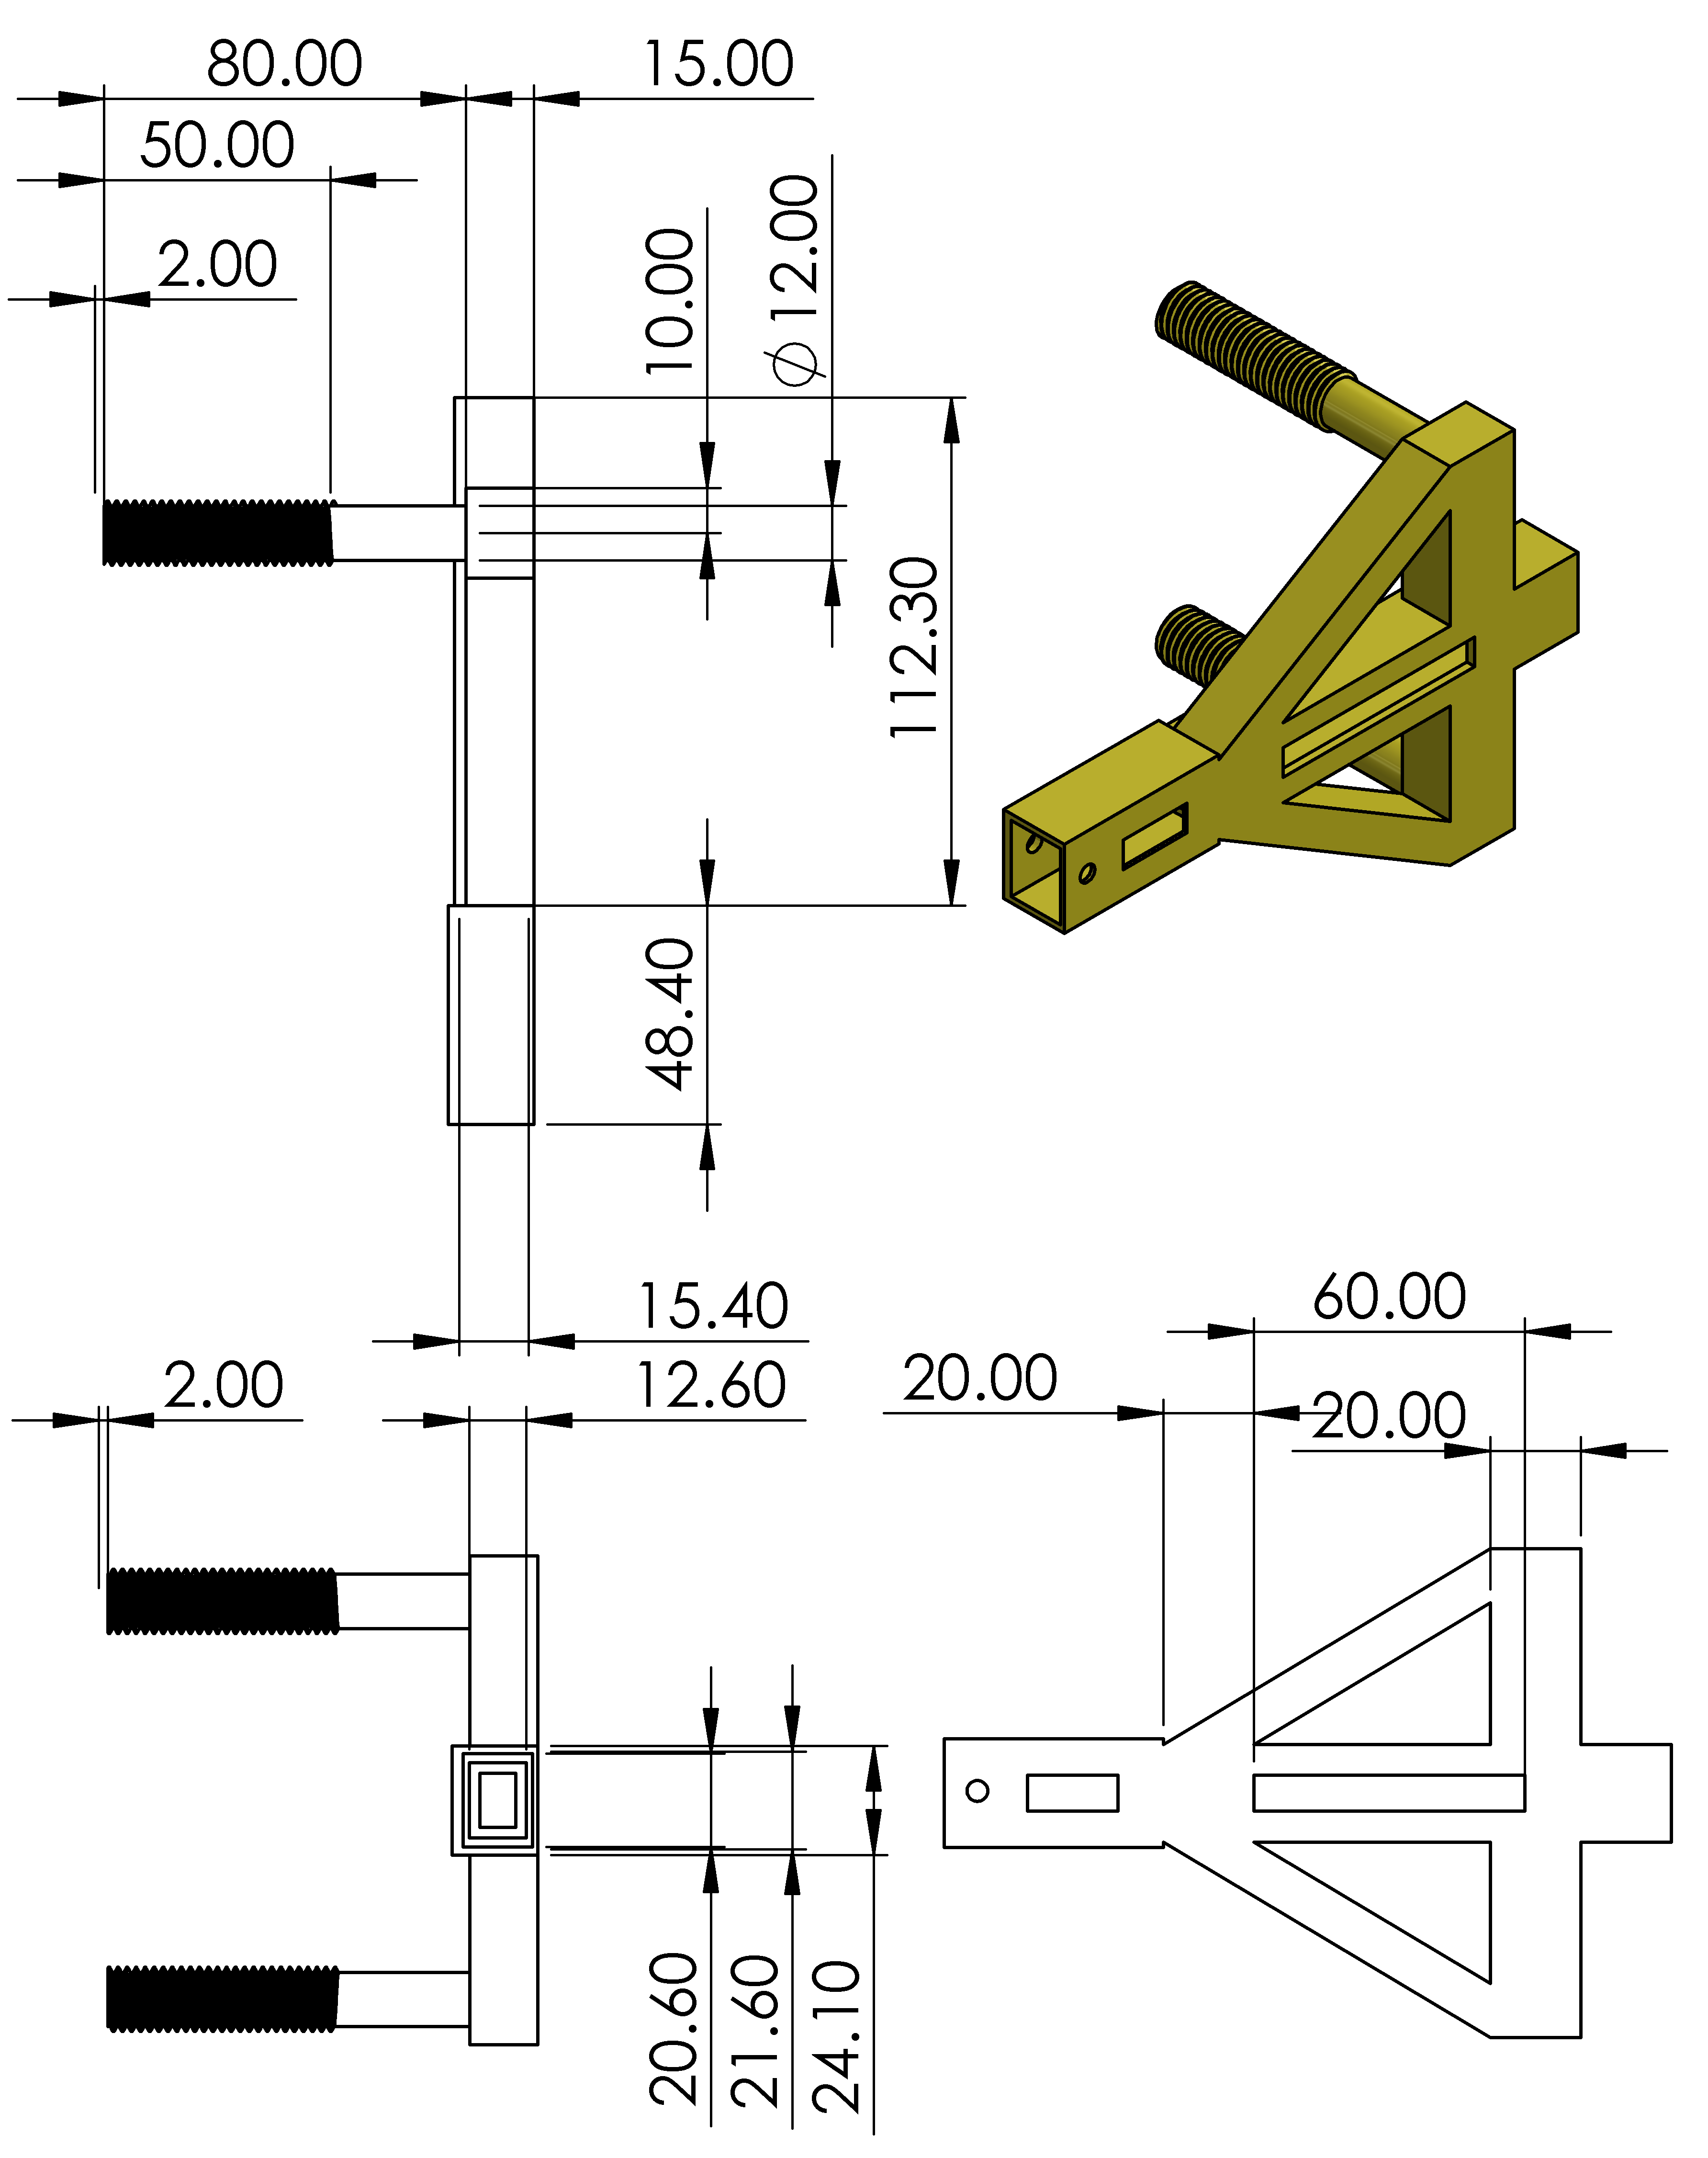
\includegraphics[height=.5\textheight]{Figures/LA-T8Holder.PNG}
        \caption{Electromagnetic actuator holder}
        \label{fig:electromagnetic_actuator}
    \end{figure}
    The dimensions of this holder design were determined from the dimensions of the LA-T8 linear actuator plus a clearance of 0.5mm.
    
    \item \textbf{Diversion Flap}
    \par
    In order to divert the flow, a channel-like flap is to be used. The design of the flap is as shown in figure \ref{fig:diversion_flap}. 
    \begin{figure}[H]
        \centering
        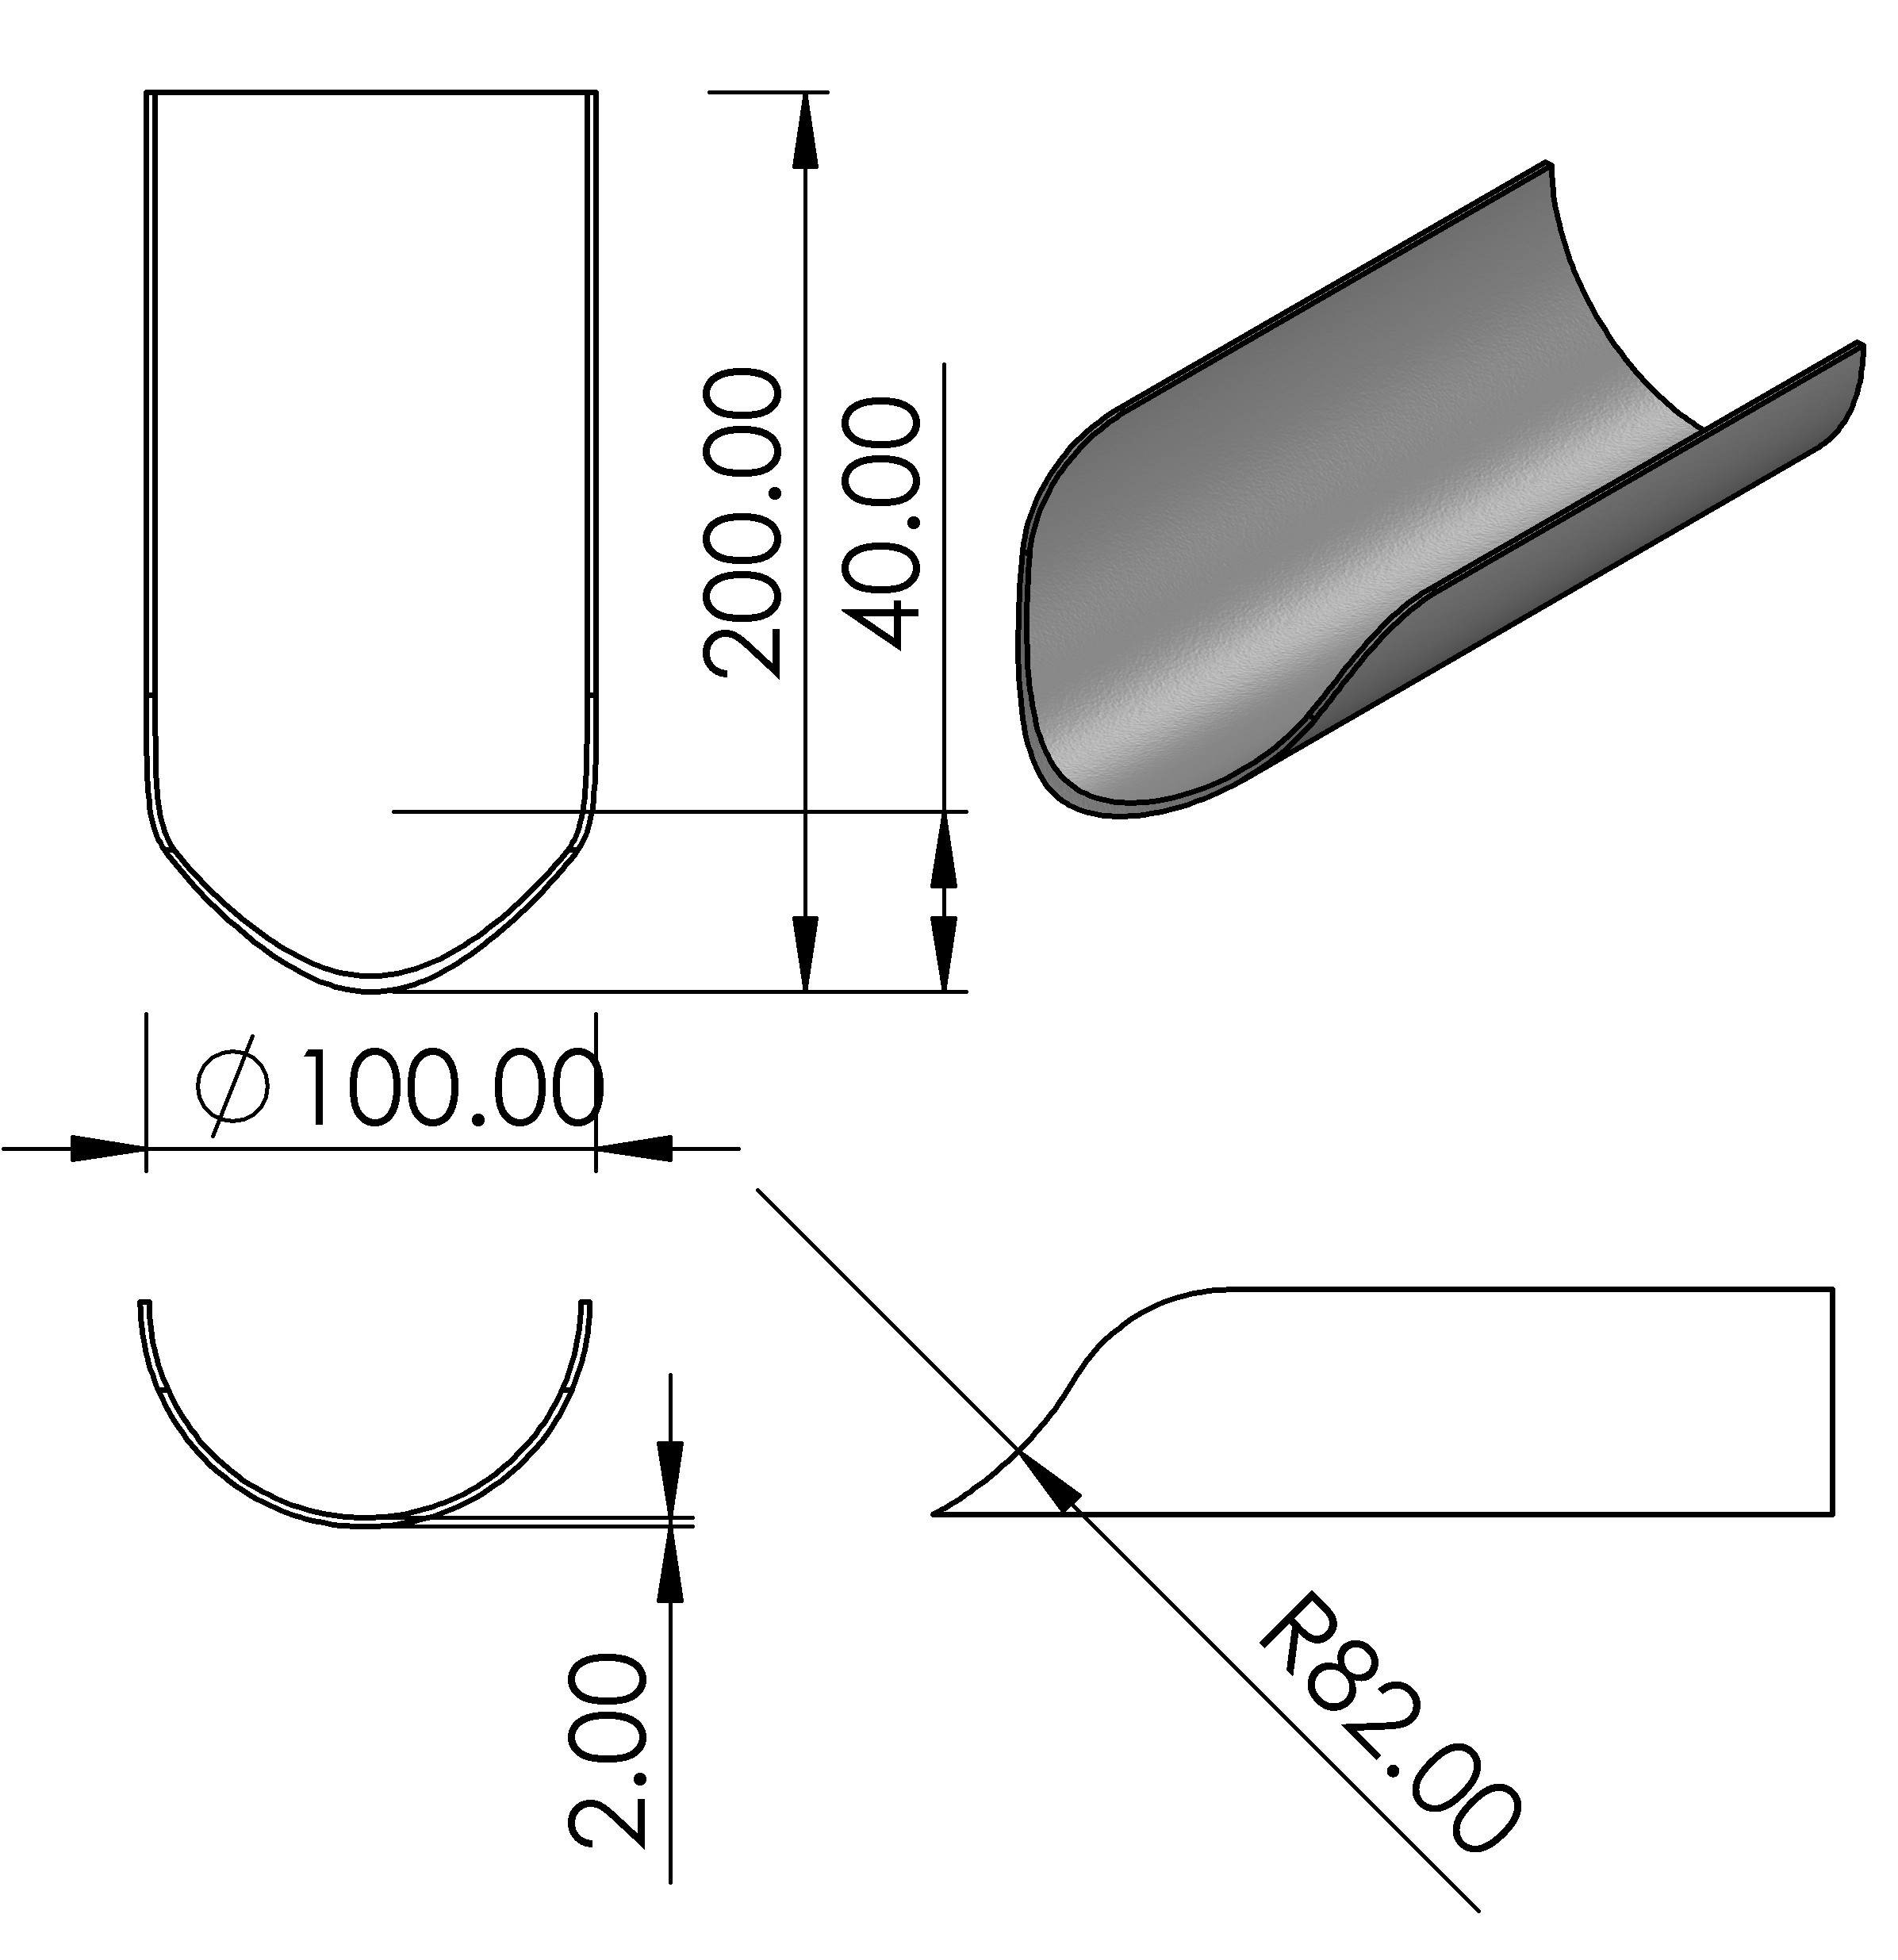
\includegraphics[height=.5\textheight]{Figures/flap2.PNG}
        \caption{Diversion flap}
        \label{fig:diversion_flap}
    \end{figure}
    The design was such that it can tap the whole stream from the $1\frac{3}{4} inch$ main discharge pipe on the main machine. Its 150mm length is determined by the length of the gap between the discharge pipe and the collection unit.
    \item \textbf{Flap support frame}
    \par
    This structure supports the diversion flap in place below the discharge pipe. This design was necessary since there is no convenient mounting point on the main machine that can allow the flap to be mounted without making changes to the main machine. It design is as shown in figure \ref{fig:flap_support_frame}.
    \begin{figure}[H]
        \centering
        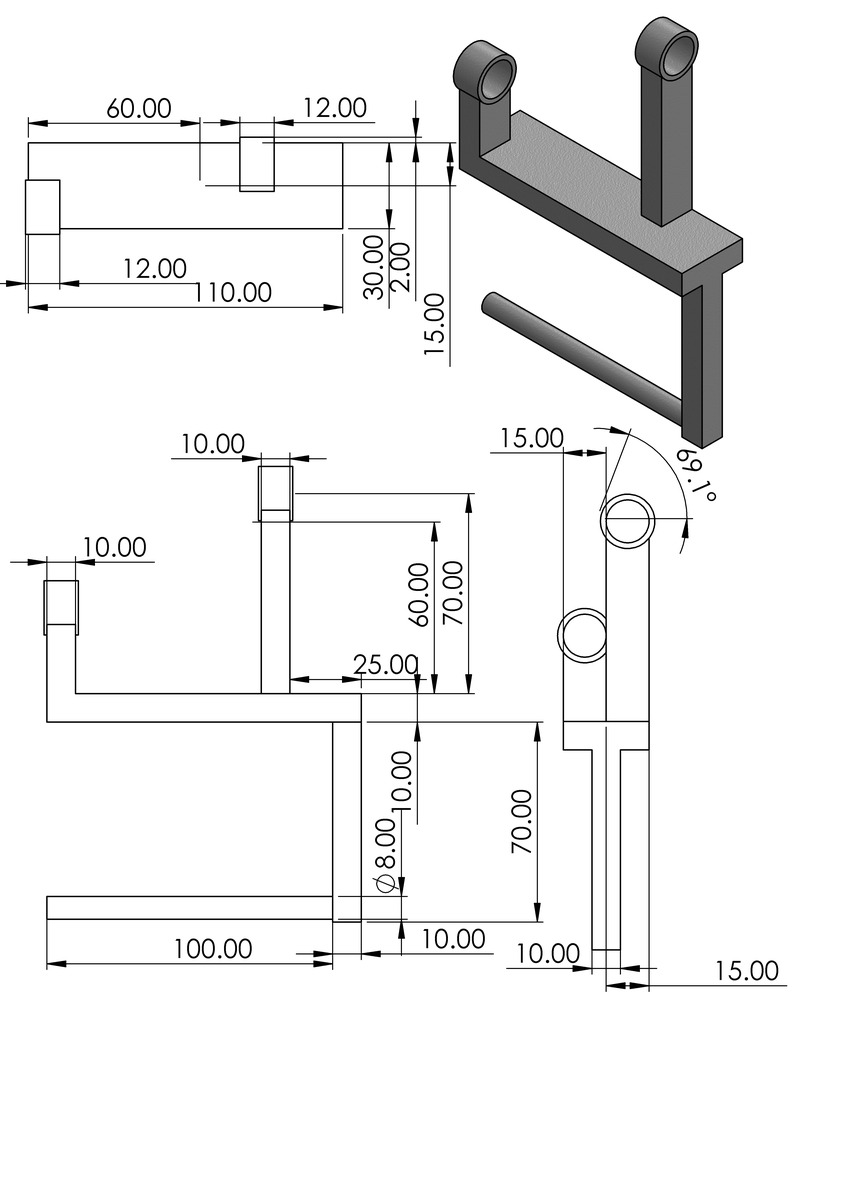
\includegraphics[height=.7\textheight]{Figures/DiversionSupport.PNG}
        \caption{Flap support frame}
        \label{fig:flap_support_frame}
    \end{figure}
    This frame also provides an extension for supporting the kinematic chain that flexes the flap. 
    \item \textbf{Link}
    \par
    The link serves to connect the linear actuator to the flap.  On one side it hinges onto the end of the 100mm actuator while on the other side it is attached to the flap. The linear movement of the actuator moves the flap to either to direct the discharge into the main reservoir or into the collection tank.
    \begin{figure}[H]
        \centering
        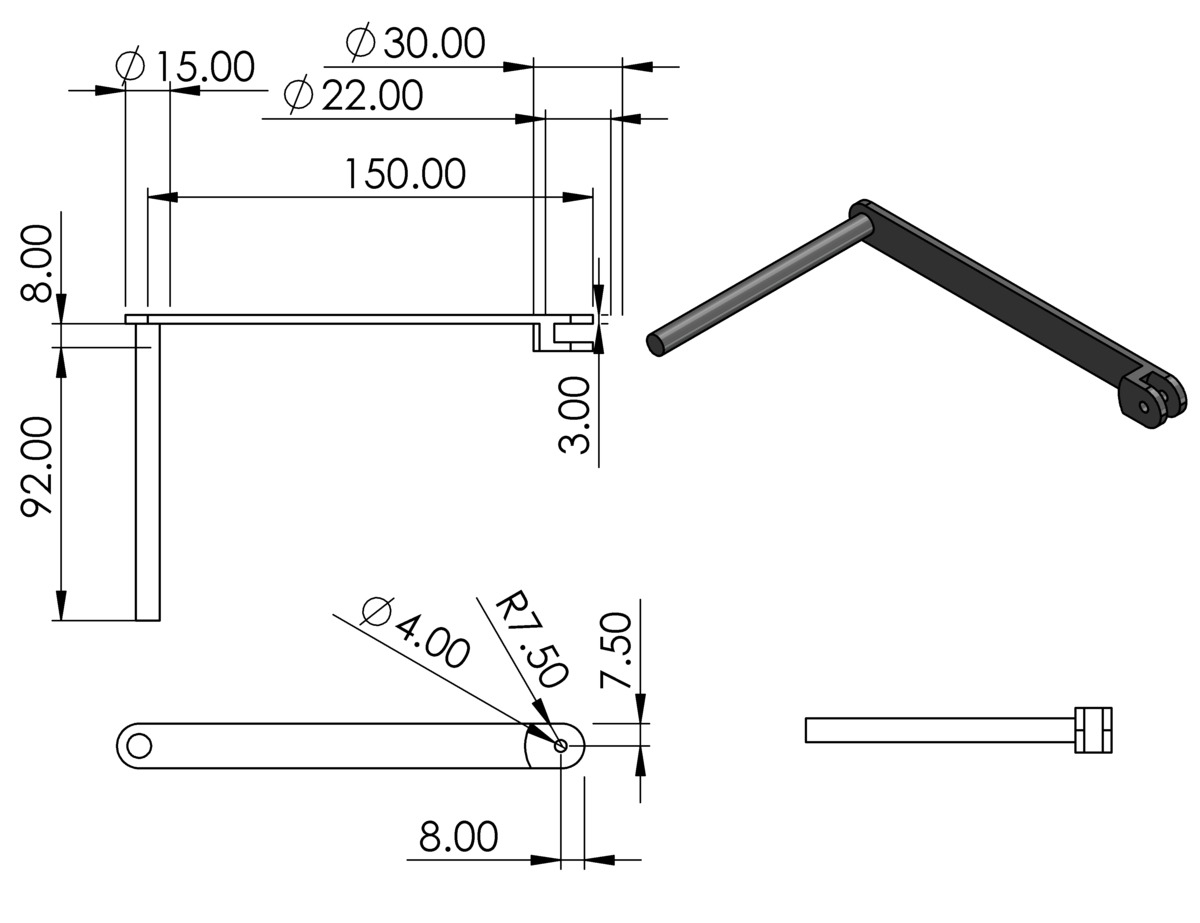
\includegraphics [width=\textwidth]{Figures/RockerLink.PNG}
        \caption{Link}
        \label{fig:my_label}
    \end{figure}
    % \par
    % To amplify the 100mm translation in order to flex the flap enough, a four-bar kinematic mechanism is used. The lengths of the links and the orientation of the four bars are determined by assuming a translation of 100mm at the output.
    % \par
    % Using the MechDesigner software, the kinematic chain was designed to provide the required motion for the flap. The CAM data from its simulation was exported automatically to a SolidWorks model of the fixed point of the part.
    % \begin{enumerate}
    %     \item \textbf{Crank}
    %     \par
    %     The input translation from the linear electromagnetic actuator. The design of this link is as shown in figure \ref{fig:crank}.
    %     \begin{figure}[H]
    %         \centering
    %         \includegraphics{Figures/KLink3.PNG}
    %         \caption{Crank}
    %         \label{fig:crank}
    %     \end{figure}
    %     The connection between this link, the end of the actuators and the couple is a series of joints. The translation is in two axes: X and Y axes.
    %     \item \textbf{Coupler}
    %     \par
    %     This link transfers the motion to the output link: the rocker. Its design is shown in Figure \ref{fig:coupler}.
    %     \begin{figure}[H]
    %         \centering
    %         \includegraphics{Figures/KLink1.PNG}
    %         \caption{Coupler}
    %         \label{fig:coupler}
    %     \end{figure}
    %     The design is such that it hinges on an extension from the flap support frame on one end and connects to the rocker on the other end. The crank is connected at a distance from one end.
    %     \item \textbf{Rocker}
    %     \par
    %     The rocker connects to the coupler on one end and to the flap on the other end. Its design is as shown in figure \ref{fig:rocker}.
    %     \begin{figure}[H]
    %         \centering
    %         \includegraphics[height=.55\textheight]{Figures/KLink2.PNG}
    %         \caption{Rocker}
    %         \label{fig:rocker}
    %     \end{figure}
    % \end{enumerate}
    % \item \textbf{Discharge flow control sub-unit}
    % \par
    % In the assembly shown in Figure \ref{fig:flow_diversion_assembly}, the flap support frame hinges on two rods: one of the servo mount rods and the other is one of the legs of the electromagnetic holder.
    % \begin{figure}[H]
    %     \centering
    %     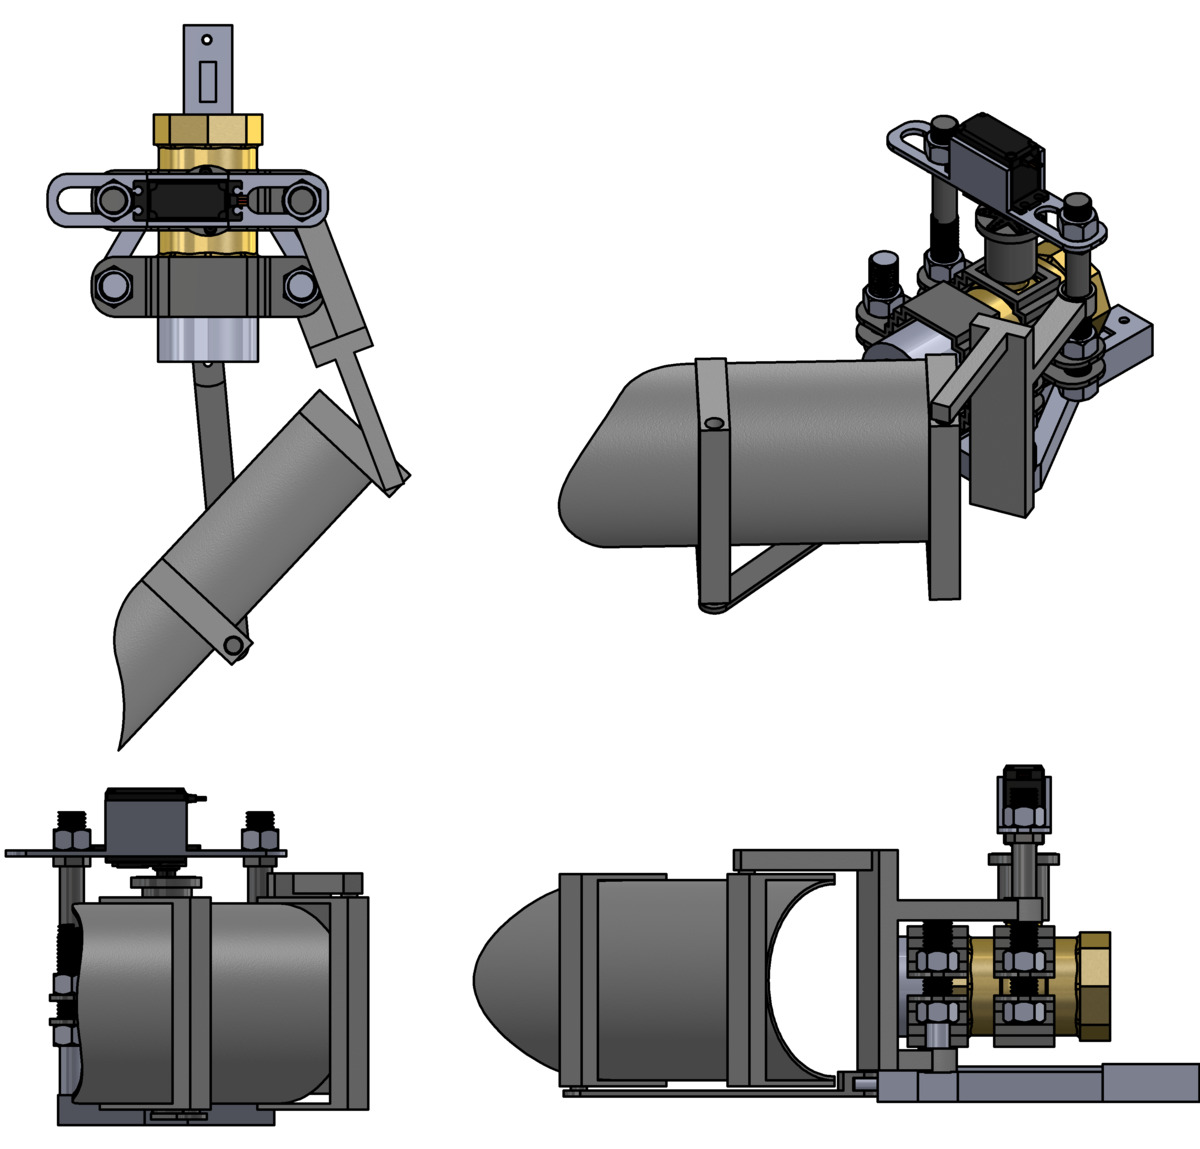
\includegraphics{Figures/DischargeFlowControlAssembly.PNG}
    %     \caption{Flow Diversion assembly}
    %     \label{fig:flow_diversion_assembly}
    % \end{figure}
    % \item \textbf{Finite element analysis of the electromagnetic actuator assembly}
    % \par
    % The finite element analysis of the assembly was performed to test how the electromagnetic diversion system is stable under a pressure force of $1N/m^{2}$ applied to the inside of the flap. PLA material was selected for all the parts in the assembly. The results of the simulation are shown in figure \ref{fig:e_simulation_results}.
    % \begin{figure}[H]
    %     \centering
    %     \includegraphics[height=\textheight, width=\textwidth]{Figures/DischargeFlowDiverSionAssembly-Static 1-1-1.png}
    %     \caption{Diversion assembly FEA results}
    %     \label{fig:e_simulation_results}
    % \end{figure}
    % From the results in figure \ref{fig:e_simulation_results}, it is evident that the electromagnetic actuator assembly holds up to the amount of distributed pressure on the flap. 
\end{enumerate}
\subsubsection{Electrical}
\begin{enumerate}
    \item \textbf{MG996R Servo motor connection}
    \par
    \begin{itemize}
        \item \textbf{Power requirements}
        \par
        From the technical specifications of the motor listed in table \ref{tab:MG996R_servo_specs}, this motor's operating voltage is 4.8V-7V, its driving current is between 500mA and 900mA, and its stall current is 2.5A(6V). However, most microcontrollers supply up to +5V DC voltage. This therefore requires a step-up circuitry or an external voltage supply to the  motor.
        \item \textbf{Connection}
        \par
        To connect an external supply requires a circuit shown in figure \ref{fig:servo_connection}.
        \begin{figure}[H]
            \centering
            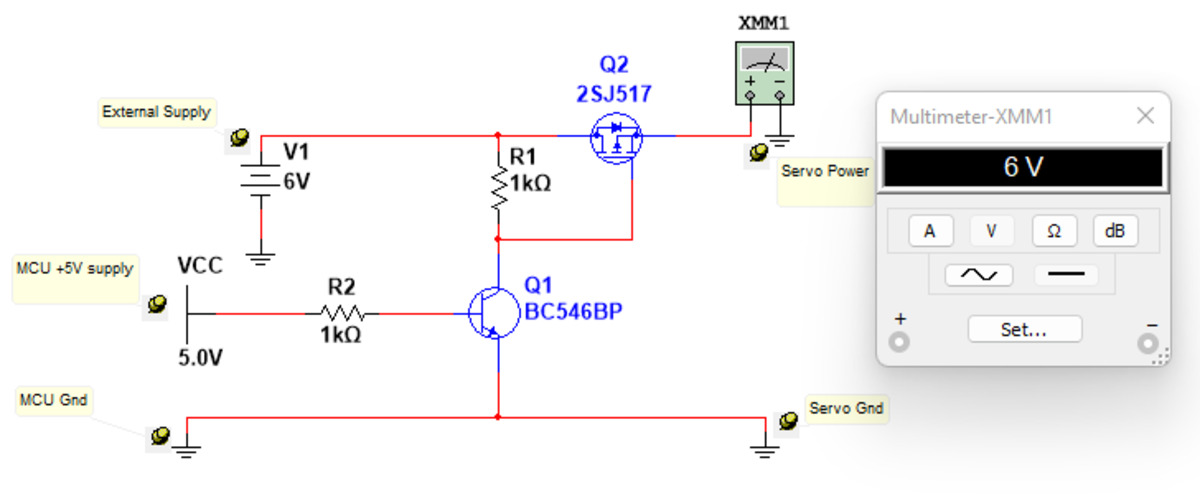
\includegraphics[width=\textwidth]{Figures/ServoConnection.png}
            \caption{Servo Connection}
            \label{fig:servo_connection}
        \end{figure}
        A 6V DC external supply is connected to the drain terminal of a Power MOSFET. This is activated by an NPN BJT transistor using the voltage supplied by the microcontroller.
    \end{itemize}
    
    \item \textbf{P16-S Electromagnetic Actuator connection}
    \par
    \begin{itemize}
        \item \textbf{Power requirement}
        \par
        The power requirements for this actuator are 12V DC supply and 2A current as listed in table \ref{tab:la_t8_tab}. These two power requirements cannot be satisfied by just a micro-controller; an external source is necessary.
        \begin{table}[H]
    \centering
       \caption[LA-T8 Micro-linear actuator technical specifications]{LA-T8 Micro-linear actuator technical specifications \cite{la_t8}}
    \begin{tabular}{|l|l|}
    \hline
    \textbf{Property} & \textbf{Value} \\ \hline
    Operating voltage & 12V DC \\ \hline
    Stroke length & 100mm \\ \hline
    Stroke speed & 150mm/s \\ \hline
    Maximum load & 6.4N \\ \hline
    \end{tabular}
    \end{table}
        \item \textbf{Connection}
        \par
        This two power requirement can be satisfied using a combination of a MOSFET power IRF520 and a D1 flyback diode as shown in Figure \ref{fig:electromagnet_connection}.
        \begin{figure}[H]
            \centering
            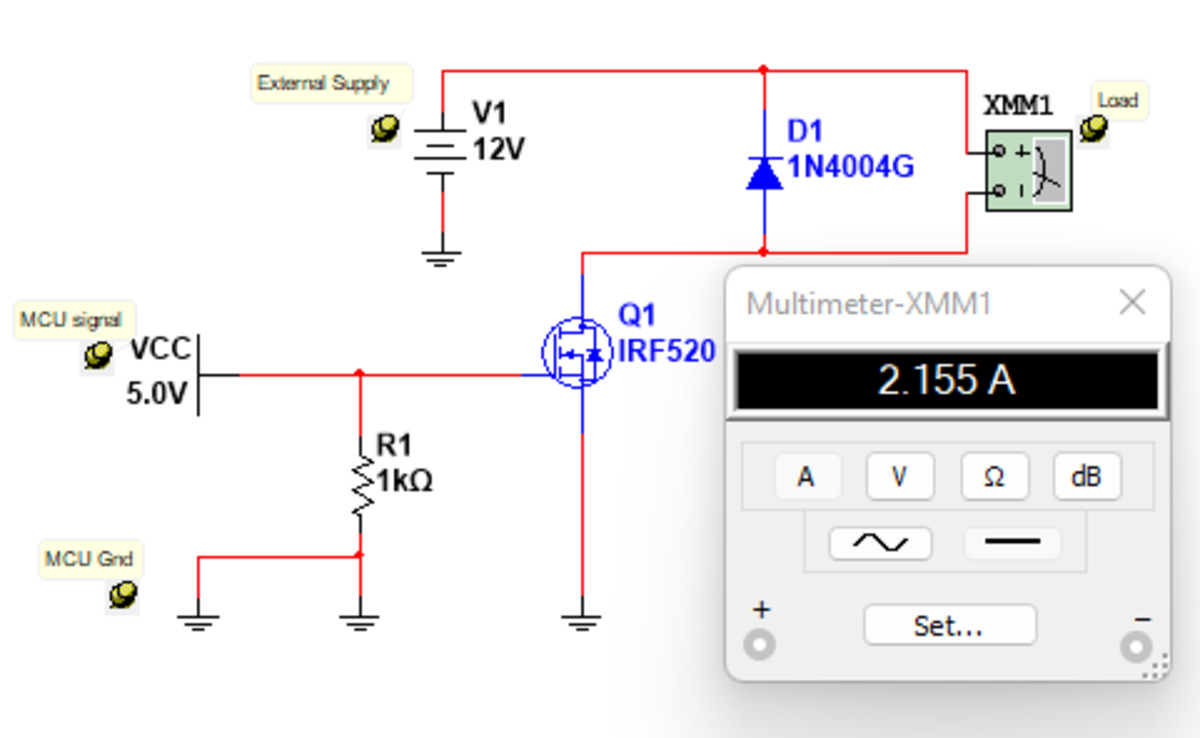
\includegraphics{Figures/ElectromagnetConnection.png}
            \caption{Electromagnetic Actuator circuit}
            \label{fig:electromagnet_connection}
        \end{figure}
        This is available in a module shown in figure \ref{fig:irf520_module}.
        \begin{figure}[H]
            \centering
            \includegraphics[width=.25\textwidth,height=.25\textheight]{Figures/IRF520Module.jpg}
            \caption[IRF520 Module]{IRF520 Module \cite{irf520}}
            \label{fig:irf520_module}
        \end{figure}
    \end{itemize}
\end{enumerate}
\subsubsection{Software and control}

\begin{enumerate}
    \item \textbf{MG996R Servo motor control}
    \par
    \begin{itemize}
        \item \textbf{Requirements}
        \par
        This motor is required to drive the ball valve in steps in a $90^{0}$ turn, the angle covered to close and open the ball valve. However, the motor can turn $120^{0}$. Therefore, the $90^{0}$ turn can be achieved by Pulse Width Modulation. 
        \item \textbf{Control}
        \par
        From the motor's datasheet, the period of the motor's control signal is 50Hz(20ms). This is checked against the clock frequency of the microcontroller and used to determine the prescaler value for the timer register.
        \par
        % For example:
        % \begin{align*}
        %     \text{Consider a micro-controller with clock frequency:} 84MHz \\
        %     Timer\_Frequency = Period \times PWM\_Frequency\\
        %     \therefore = 20000 \times 50 Hz  = 1MHz\\
        %     Pre-scaler = \frac{Clock\_frequency}{Timer\_frequency}\\
        %     \therefore = \frac{84}{1} = 84
        % \end{align*}
        % The angle turned by the motor is proportional to the Logic HIGH duty. Therefore, by writing a time value for $90^{0}$ full turn in the timer register, the turn can be achieved. Smaller turns can be achieved by writing corresponding time values to the timer register.
    \end{itemize}
    \item \textbf{LA-T8 electromagnetic Actuator control}
    \par
    \begin{itemize}
        \item \textbf{Requirements}
        \par
        In order to divert the flow, this actuator is required to provide a linear stroke and remain in position for a set amount of time. When the time elapse, it is required to linearly retract in order to restore the flow. 
        \item \textbf{Control}
        \par
        This actuator provides a full length stroke in;
        \begin{align*}
            \text{Full length of a stroke: } = 100mm\\
            Stroke\_speed = 150mm/s\\
            \therefore \text{Time taken for a full length stroke is} \frac{10}{15}^{th}  \text{of a second.}
        \end{align*}
        This is achieved when it is powered. The terminals are switched in order to retract it.
        \par
        Shorter strokes can be achieved by turning on the actuator for a time less than $\frac{10}{15}$ \textit{th} seconds.
    \end{itemize}
\end{enumerate}
Controlling these two electronics requires an RTOS platform. There are many RTOS platforms but Zephyr and Mbed platforms are preferred because of their relatively large support with extensive APIs. 
\clearpage
\subsection{Discharge Handling Unit}
This unit consists of the following subunits:
\begin{enumerate}
    \item Discharge collection tank sub-unit.
    \item Outlet valve sub-unit.
    \item Weight measurement sub-unit.
    \item Temperature measurement sub-unit.
\end{enumerate}

\subsubsection{Discharge collection tank sub-unit}
\begin{itemize}
\item \textbf{Collection tank}
\par
This is used to temporarily collect the discharge from the pipeline during each step of an experiment, after which it is released to the main reservoir through an outlet valve. The weight and temperature of the discharge are also taken in this tank. 
\par
The following design considerations were made when selecting a tank for this application.
\begin{enumerate}
    \item Shape of the tank 
    \par
    The design of this tank should be such that the tank discharges in the least time possible with no remnants. Therefore, the shape of the tank was put into much consideration such that it influences/motivates the discharge. The following shapes were taken into consideration.
    \par
    \begin{itemize}
        \item \textbf{Cuboid tank}
        \par
    The design of the tank is shown in Figure \ref{fig:cuboid_discharge_container}.
    \begin{figure}[H]
        \centering
        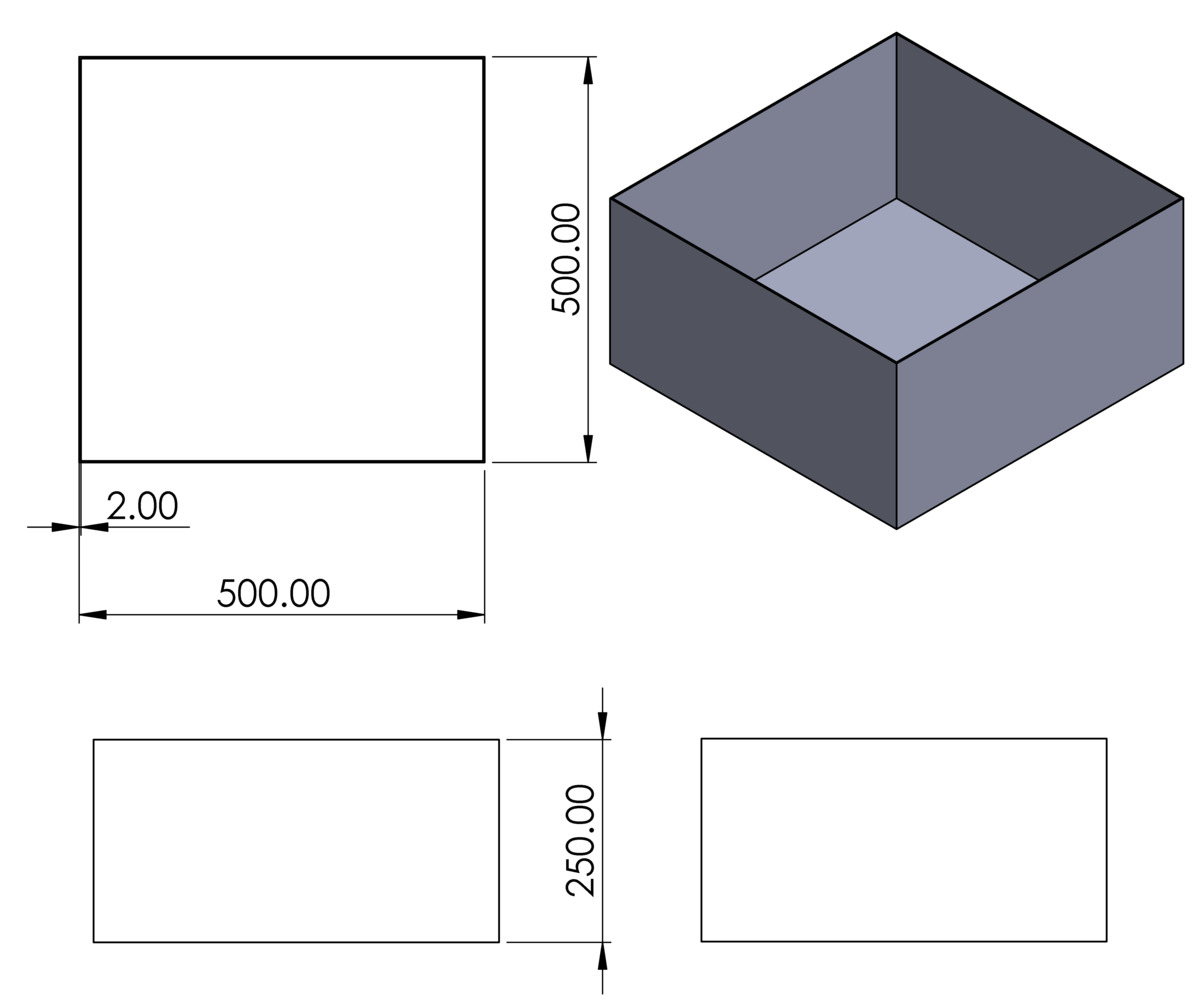
\includegraphics[height=.4\textheight]{Figures/DischargeContainer.PNG}
        \caption{Cuboid discharge container}
        \label{fig:cuboid_discharge_container}
    \end{figure}
    This tank satisfies the requirements for this application. However, a small volume of discharge will tend to remain in the tank when the tank is emptied.
        \item  \textbf{Horizontal Cylindrical tank}
    \end{itemize}
    \begin{figure}[H]
        \centering
        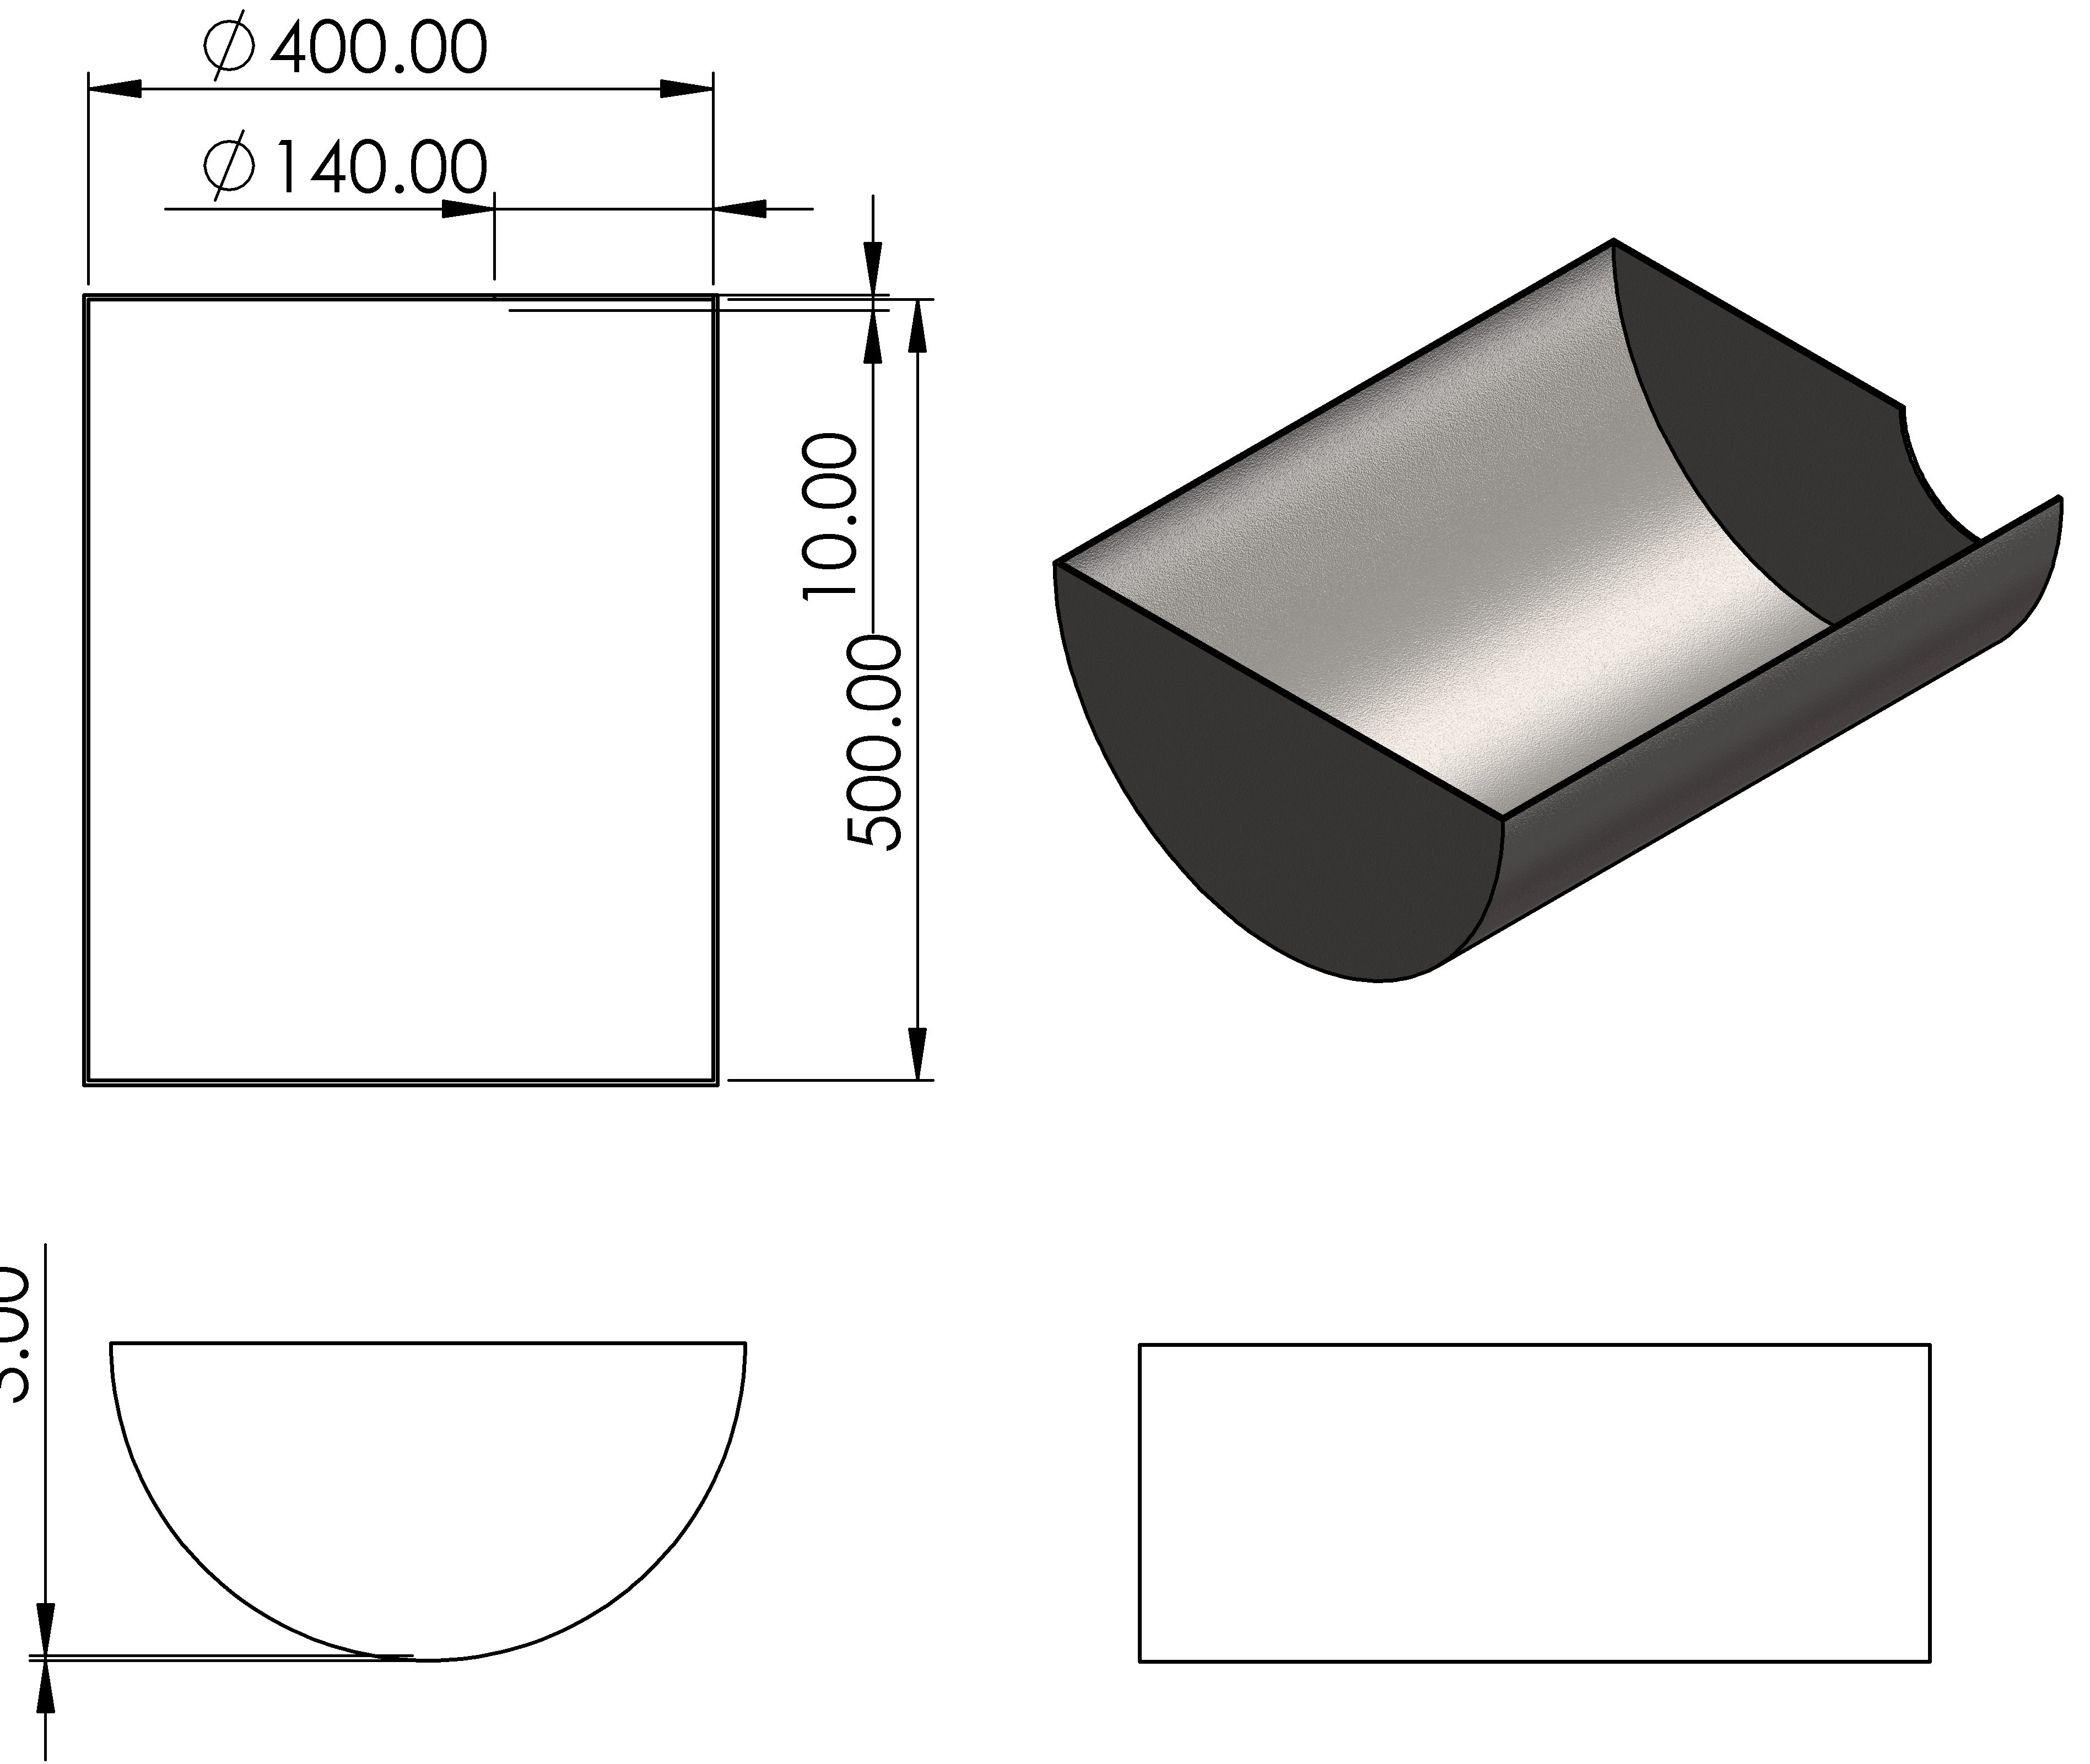
\includegraphics[height=.25\textheight]{Figures/tank.PNG}
        \caption{Horizontal Cylindrical tank}
        \label{fig:horizontal_cylindrical_tank}
    \end{figure}
    When emptying this tank, the tank motivates the flow out of the discharge due to the concentration of the pressure of the discharge on a line at the bottom of the container determined by a static simulation.
    \par
    The horizontal cylindrical tank was selected for this application.
    \item Material of the tank
    \par
   The collection tank will hold the discharge from the pipeline. It was key to ensure that the tank was corrosion resistant to avoid issues with rust. Taking the above into consideration, stainless steel and mild steel were considered to be used in the fabrication of the tank. There comparisons are discussed below.
   \begin{table}[H]
    \centering
      \caption[Stainless Steel Versus Mild Steel]{Comparison between Stainless Steel and Mild Steel}
    \begin{tabular}{|m{3cm}|m{5cm}|m{5cm}|}
    \hline
Parameters & Stainless Steel &  Mild Steel \\ \hline 
Corrosion Resistant &  Much higher corrosion resistance &  Lower corrosion resistance (Require further processing such as galvanising in order to give it a protective surface) \\ \hline
Fabrication & Much more impact resistant compared to mild steel  & Much more malleable compared to stainless and so is used a lot in general fabrication.\\ \hline
Cost & Expensive & Cheaper\\ \hline
    \end{tabular}
    \end{table}
 \par
 Mild steel was selected to be used in the fabrication of the collection tank due to malleability hence ease of fabrication and cost. However, secondary operations in this case painting will be done to prevent corrosion.
 
    \item Volume of the tank
    \par
    The volume of the tank tank was such that it can hold a stream from the $1 \frac{3}{4} inch$ main discharge pipe that flows for approximately 30 seconds when the valve is fully opened. This was around $0.01m^{3}$. Therefore, the dimensions of the tank were such that it produced a volume of this value.
\end{enumerate}
% Based on the above considerations, two options were technically feasible in terms of the available means for fabrication:
% \begin{enumerate}
%     \item \textbf{Cuboid tank}
%     \par
%     The design of the tank is shown in Figure \ref{fig:cuboid_discharge_container}.
%     \begin{figure}[H]
%         \centering
%         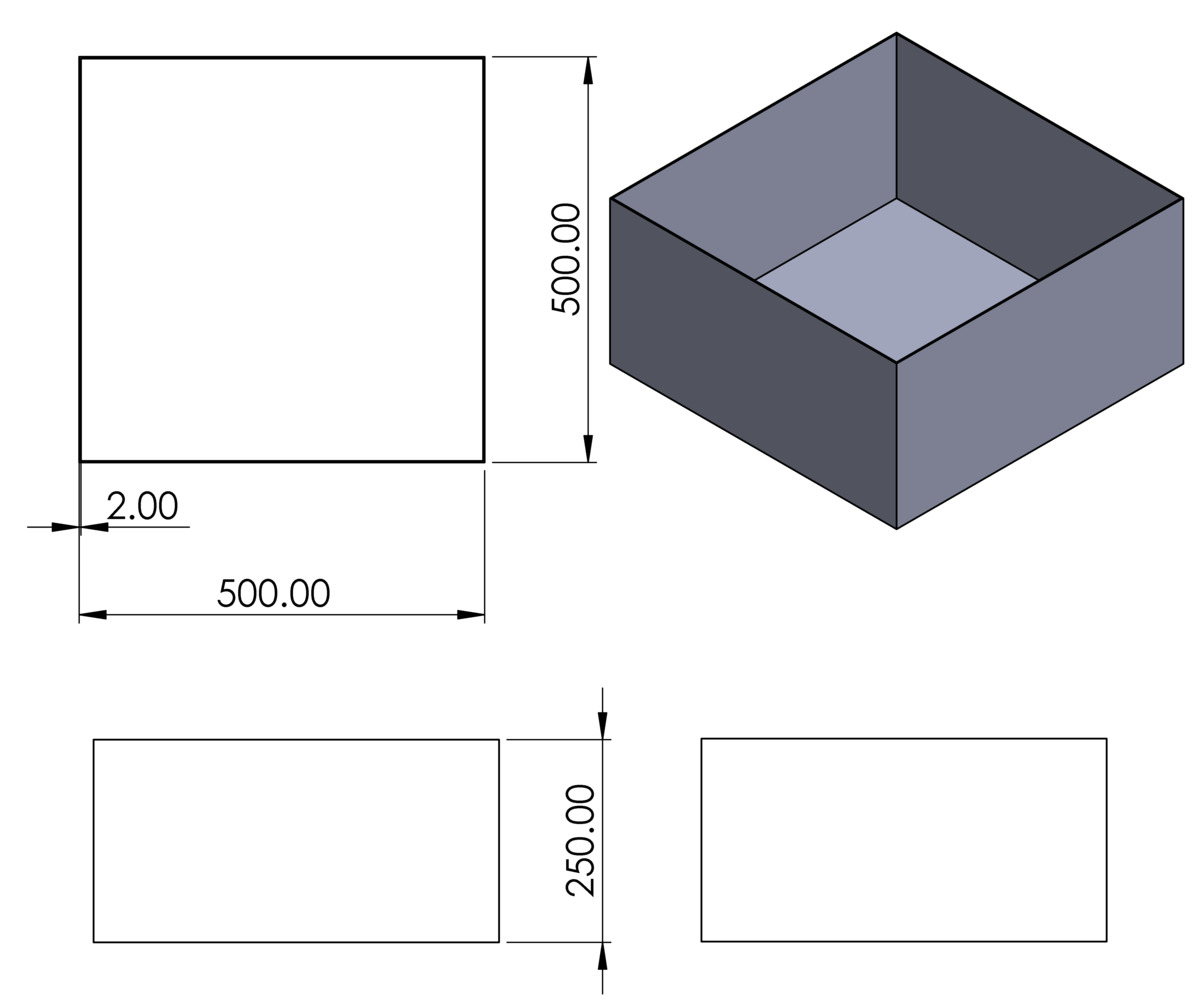
\includegraphics[height=.4\textheight]{Figures/DischargeContainer.PNG}
%         \caption{Cuboid discharge container}
%         \label{fig:cuboid_discharge_container}
%     \end{figure}
%     This tank satisfies the requirements for this application. However, a small volume of discharge will tend to remain in the tank when the tank is emptied.
%     \item \textbf{Horizontal Cylindrical tank}
%     \par
%     The design of this tank is shown in Figure \ref{fig:horizontal_cylindrical_tank}.
%     \begin{figure}[H]
%         \centering
%         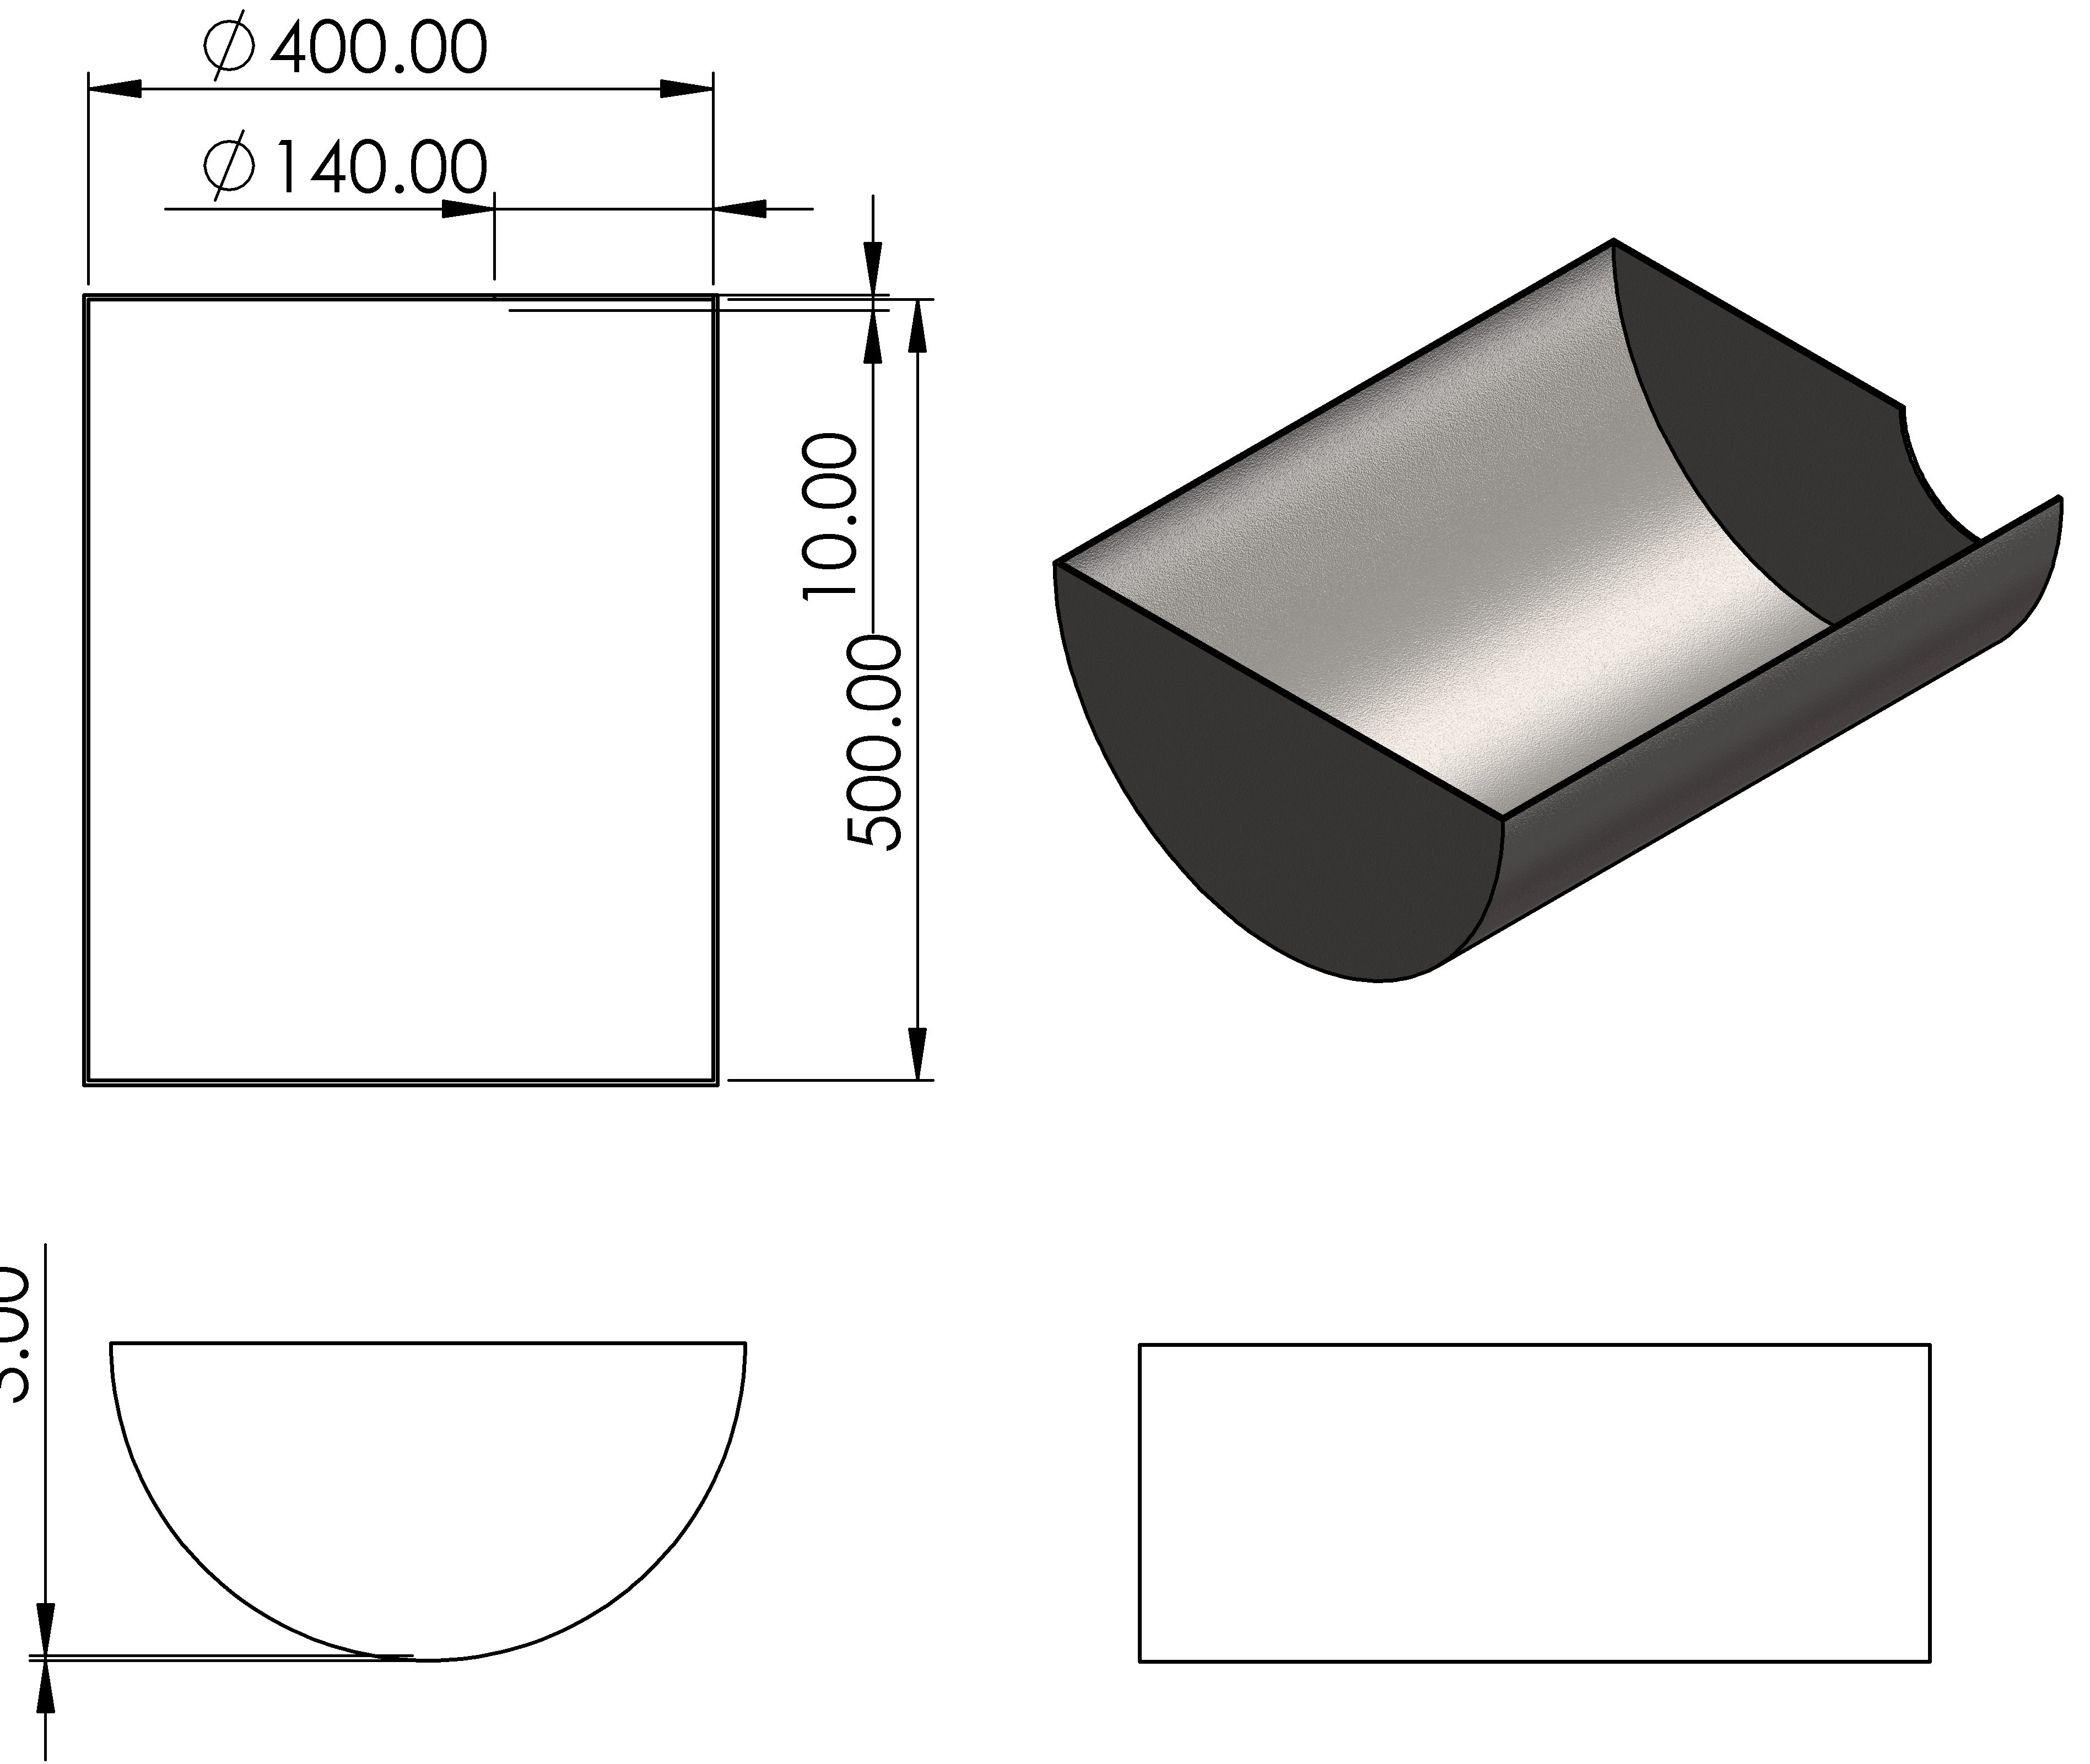
\includegraphics[height=.25\textheight]{Figures/tank.PNG}
%         \caption{Horizontal Cylindrical tank}
%         \label{fig:horizontal_cylindrical_tank}
%     \end{figure}
%     When emptying this tank, the tank motivates the flow out of the discharge due to the concentration of the pressure of the discharge on a line at the bottom of the container determined by a static simulation.
%     % \begin{figure}[H]
%     %     \centering
%     %     \includegraphics[width=\textwidth, height=.4\textheight]{Figures/tank-Static-1-1-1.png}
%     %     \caption{Tank simulation results}
%     %     \label{fig:tank_simulation_results}
%     % \end{figure}
% \end{enumerate}


\par
\item \textbf{Tank support frame}
\par
In order to support the tank in an upright position on a flat surface a support frame shown in figure \ref{fig:cylindrical_tank_support_frame}.

\begin{figure}[H]
    \centering
    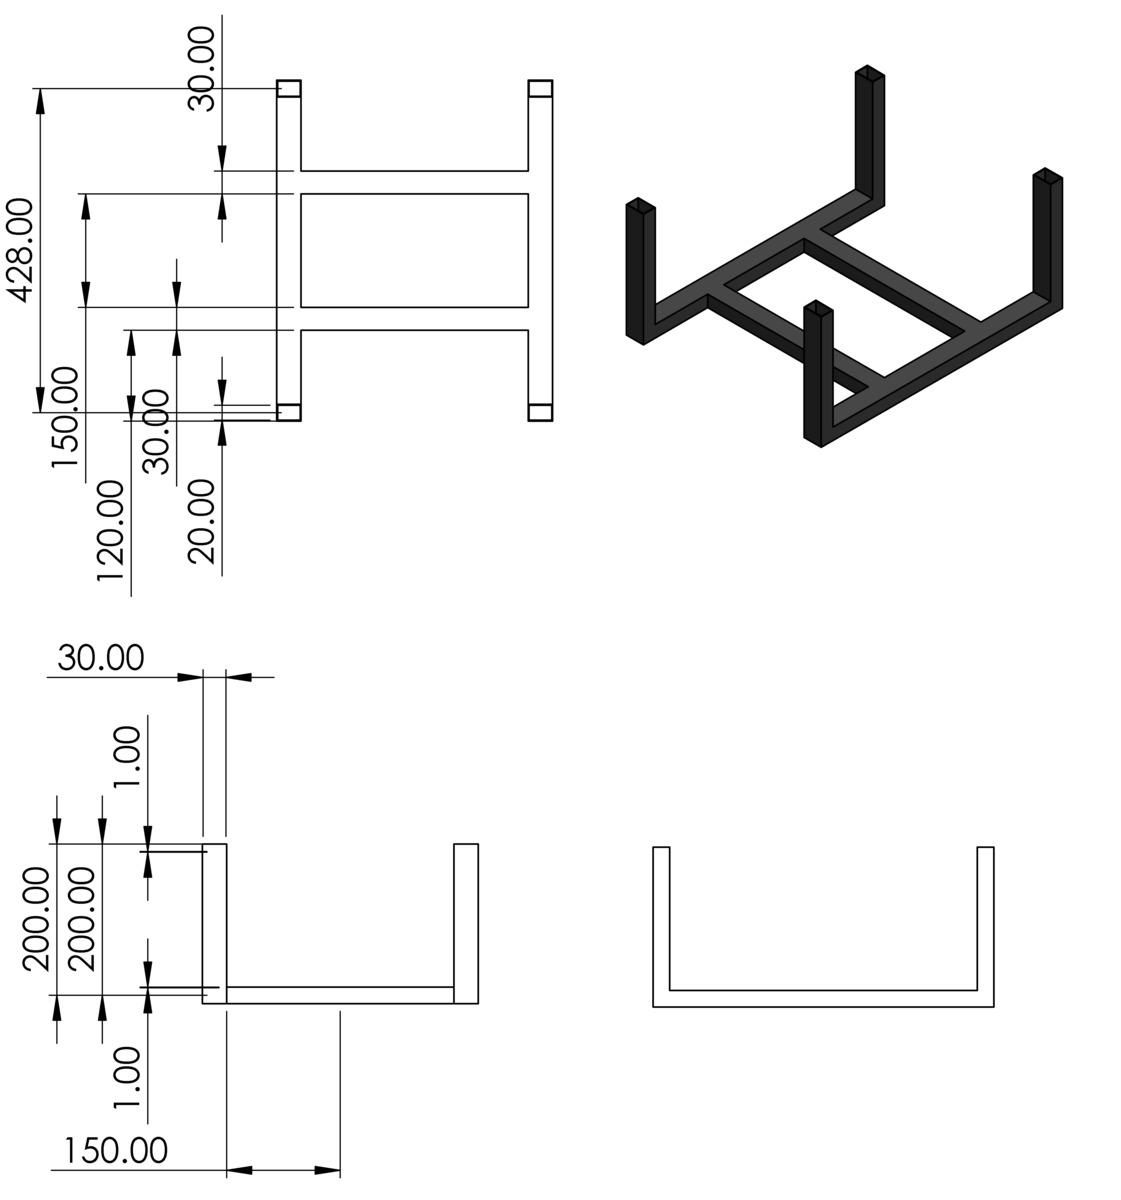
\includegraphics[height=.55\textheight]{Figures/tankHolder.PNG}
    \caption{Cylindrical tank support frame}
    \label{fig:cylindrical_tank_support_frame}
\end{figure}

The dimensions of the frame were such that it provides a clearance of 1mm for the tank.

\par
\item \textbf{Tank assembly}
\par
The assembly of the tank and its support frame are as shown in figure \ref{fig:collection_tank}.
\begin{figure}[H]
    \centering
    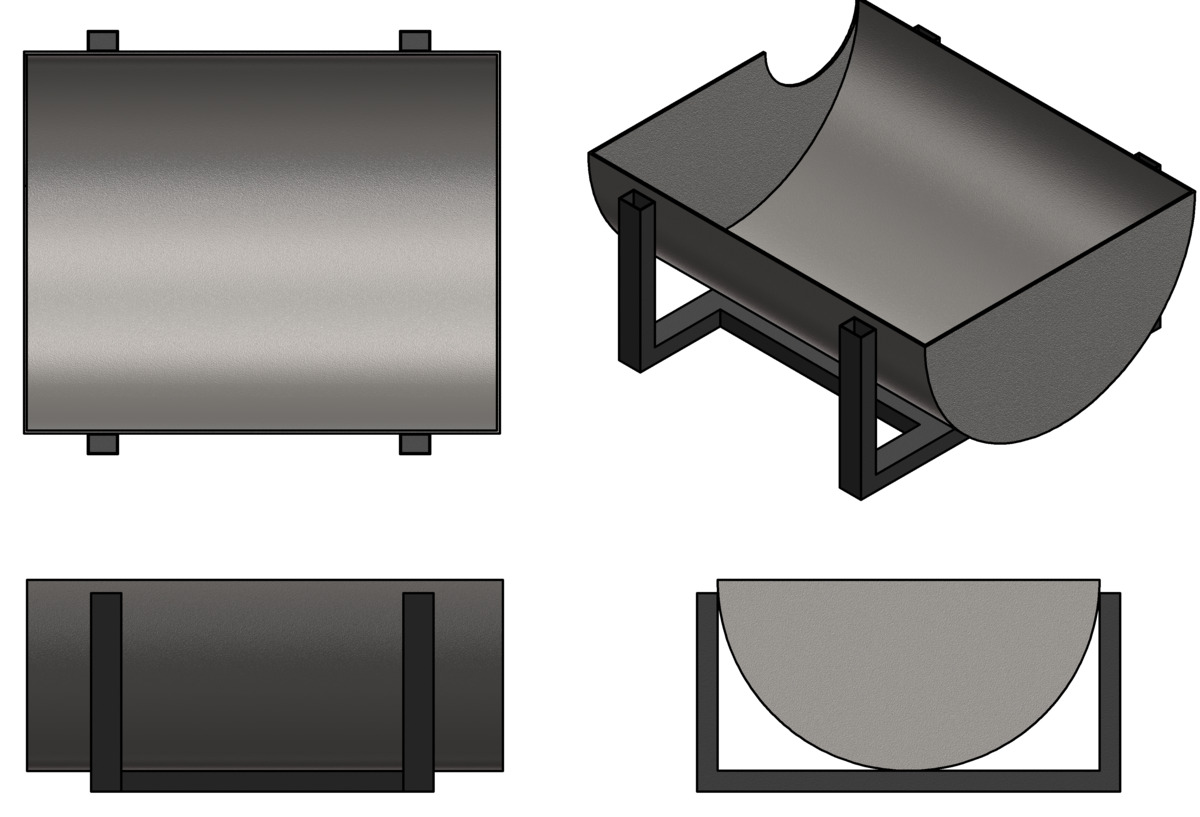
\includegraphics[height=.45\textheight]{Figures/CollectionTank.PNG}
    \caption{Collection tank}
    \label{fig:collection_tank}
\end{figure}
\par
\item \textbf{Position}
\par
The positioning of the tank was also a critical aspect of the design. Ideally, the collection tank was to be either positioned directly just below the flow diversion unit or at the periphery of the main reservoir. Positioning the collection tank directly below the flow diversion unit mitigates the need for additional components such as diverting pipes. This simply implies that the collection tank would just be provided with a holding mechanism for support upon which it is fitted with a solenoid outlet valve directly into the reservoir. On the contrary, positioning the collection tank on the periphery introduces the need for additional components. This includes a pump system to pump the discharge back into the reservoir, which adds to the overall cost of the project. Positioning the collection tank below the diversion unit was the feasible option due to cost considerations.
\end{itemize}

\subsubsection{Outlet valve sub-unit}
It is used to empty the tank into the main reservoir. The main consideration was the response time(time taken to close and open the valve) in the selection of a valve suitable for this application. The following options were feasible:
\begin{enumerate}
    \item \textbf{An electrically Controlled Butterfly valve}
    \par
    \begin{figure}[H]
        \centering
        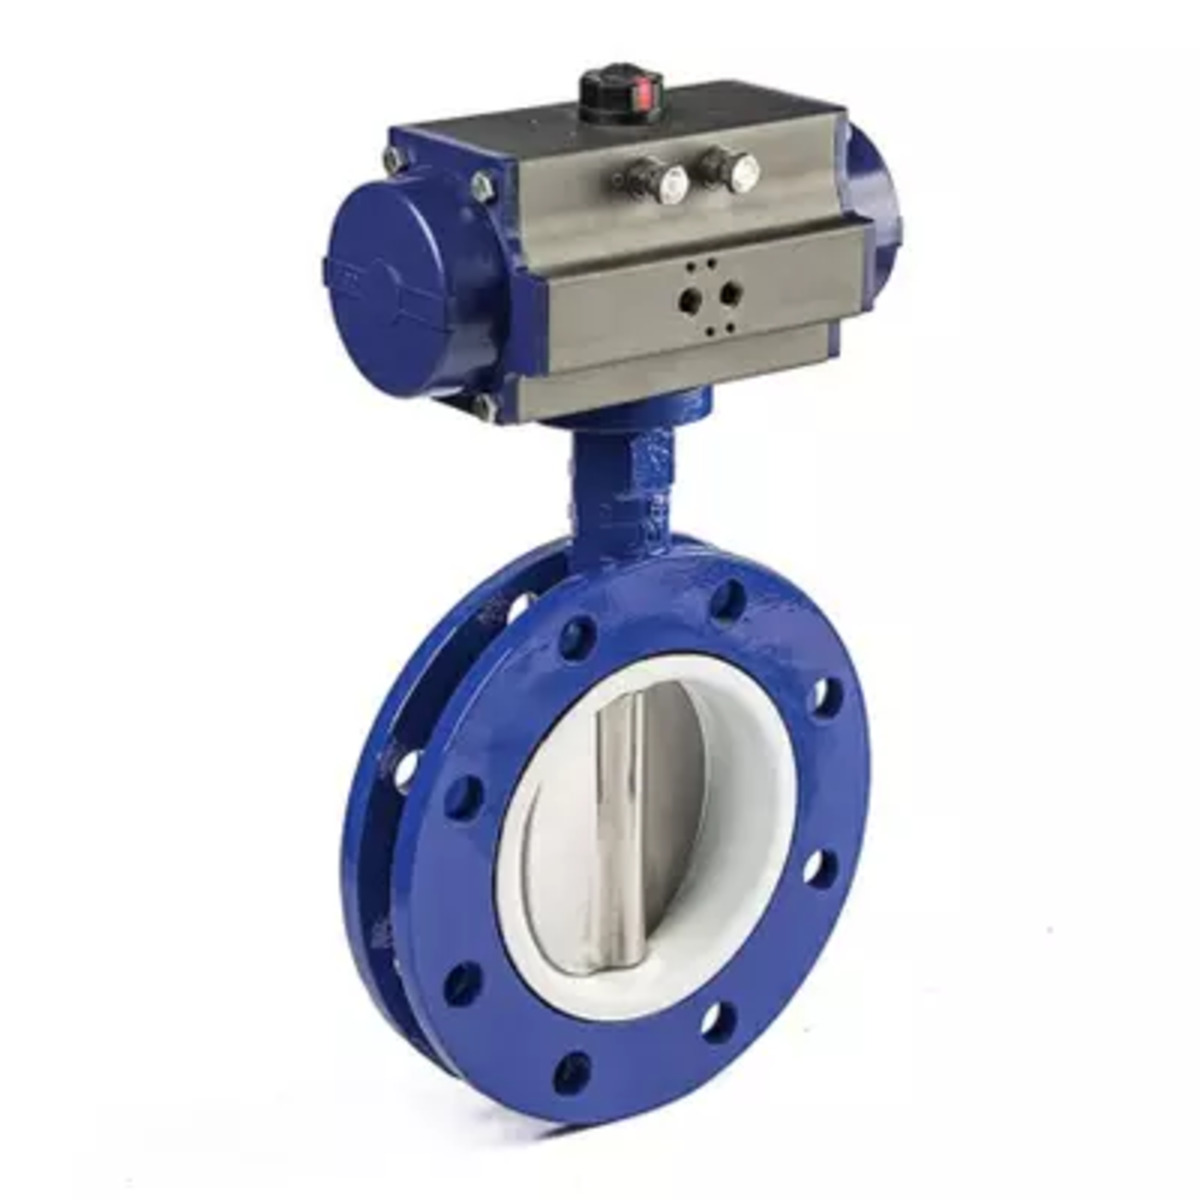
\includegraphics[width=0.2\textwidth, height=.2\textheight]{Figures/butterflyValve.png}
        \caption[Butterfly valve]{Butterfly valve \cite{butterfly}}
        \label{fig:butterfly_valve}
    \end{figure}
    The operating voltage of the valve shown in figure \ref{fig:butterfly_valve} is in the range 12V DC - 230V AC. Therefore, its response time can be reduced by increasing the voltage supply to the solenoid.
    \item \textbf{A solenoid gate valve(with a plunger)}
    \par
    \begin{figure}[H]
        \centering
        \includegraphics[width=.2\textwidth, height=.2\textheight]{Figures/solenoidValve.jpg}
        \caption[Solenoid valve]{Solenoid valve \cite{solenoid}}
        \label{fig:solenoid_valve}
    \end{figure}
    The $\frac{3}{4} inch$ solenoid valve shown in figure \ref{fig:solenoid_valve} uses a plunger with a cork for control the flow. How fast the plunger closes the aperture depends on the voltage supplied to the solenoid. The operating voltage of this type of valve is 12V DC.
\end{enumerate}

The solenoid gate valve(with a plunger) was selected for this application mainly because the butterfly valve is expensive relative to the budget set for the project.

\subsubsection{Weight measurement sub-unit}
The weight of the collected discharge is measured in every step of the experiment. Weight measurement is cumulative. In the event of an error, the error is not propagated in the cumulative approach unlike in the weight-per-step approach. Therefore, the cumulative approach was selected for this application.
\par
The selection of the weight measurement device was guided by the following considerations:
\begin{enumerate}
    \item The maximum weight that can be precisely measured by the unit. The maximum weight of the structure to be measured is determined as follows:\\
    \begin{align*}
    \text{Assume the maximum volume of the water collected} = 0.02m^{3}.\\
    Mass(M) = Density(\rho) \times Volume(V)\\
    \text{Water density} (\rho_{\textit{water}}) = 1000kg/m^{3}\\
    \therefore  \text{Mass of water} (M_{\textit{water}}) = 20 Kg
    \end{align*}
    The measuring device should therefore handle weights of more than 20Kg.
    \item The resolution of the device.
\end{enumerate}
On the basis of the above considerations, the following options were considered:
\begin{enumerate}
    \item Weight measurement by ultrasonic waves
    \par
    Ultrasonic waves can be used to determine the depth of discharge in the tank. The time taken to send and receive the echo is multiplied by the speed of sound to obtain the depth of the empty side of the container. However, to use this approach requires calibration of several parameters, some of which are to be done in real time. A mathematical model would be preferable for this calibrations. 
    % This approach is rudimentary and very much flawed as there are many considerations in order to obtain almost accurate results. Some of the considerations include:
    % \begin{enumerate}
    %     \item The angle of reflexion $\delta$ is shown in figure \ref{fig:ultrasonic sensor measurement model}.
    %     \begin{figure}[H]
    %         \centering
    %         \includegraphics{Figures/angleOfReflection-1.png}
    %         \caption[Ultrasonic sensor measurement model]{Ultrasonic sensor measurement model \cite{chang1996ultrasonic}}
    %         \label{fig:ultrasonic sensor measurement model}
    %     \end{figure}
    %     \item The Gaussian noise to environmental changes. There is an almost 3.5\% increase in noise for a temperature difference of only $20^{0}$ \cite{chang1996ultrasonic}.
    % \end{enumerate}
   
    \item Load cells
    % \par
    % These are transducers capable of converting pressure to an electrical signal specifically a strain in its material structure is converted to electrical resistance.
    \par
    The loading cell disc shown in Figure \ref{fig:load_cell_disc} with a load force range of 0-50Kg was selected for application due to its weight range.
    \begin{figure}[H]
        \centering
        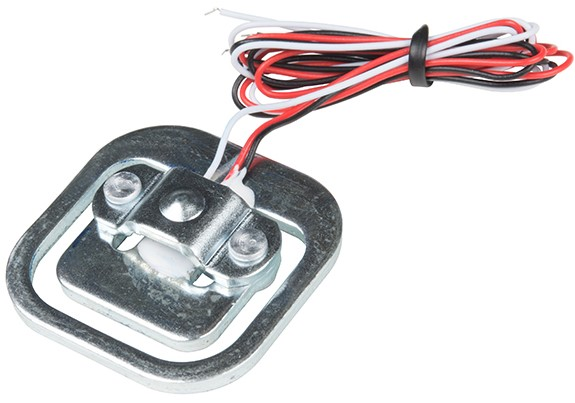
\includegraphics[width=.25\textwidth, height=.25\textheight]{Figures/50KgLoadCell.jpg}
        \caption[Strain-type load cells]{Strain-type load cells \cite{loadcell}}
        \label{fig:load_cell_disc}
    \end{figure}
\end{enumerate}
 Four load cells  will be strategically positioned at the edges of the support frame of the discharge collection tank, as shown in Figure \ref{fig:collection_tank_with_load_cells}.
\begin{figure}[H]
    \centering
    \includegraphics[height=.45\textheight]{Figures/CollectionTankWithTheLoadCells.PNG}
    \caption{Collection tank with load cells}
    \label{fig:collection_tank_with_load_cells}
\end{figure}

\subsubsection{Temperature measurement sub-unit}
 The temperature of the discharge is measure in every step to ensure consistency of the data collected. Since this measurement is taken within roughly 10 seconds before the outlet valve is opened, a measuring device whose sensitivity is enough to establish reliable results within that time is required for this application. An immersible DS18B20 temperature probe shown in figure \ref{fig:ds18b20_temperature} was selected. Its technical specifications are shown in table \ref{tab:ds18b20 temperature probe}.
\begin{figure}[H]
    \centering
    \includegraphics[width=.28\textwidth, height=.28\textheight]{Figures/ds18b20_temperature_probe.jpg}
    \caption[DS18B20 temperature probe]{DS18B20 temperature probe \cite{ds18b20}}
    \label{fig:ds18b20_temperature}
\end{figure}
\begin{table}[H]
\centering
\caption[DS18B20 temperature range specifications]{DS18B20 temperature range specifications \cite{ds18b20}}
\begin{tabular}{|l|l|}
\hline
\textbf{Property} & \textbf{Value} \\ \hline
Operating voltage & 3.3V  to 5V DC \\ \hline
Operating temperature range & -55°C to +125°C (-67°F to +257°F) \\ \hline
Accuracy over the range of -10°C to +85°C: & ±0.5°C. \\ \hline
Water proof & True \\ \hline
\end{tabular}
\label{tab:ds18b20 temperature probe}
\end{table}

\subsubsection{Electrical}
\begin{enumerate}
    \item \textbf{Solenoid valve connection}
    \par
    \begin{itemize}
        \item \textbf{Power requirements}
        \par
        The selected solenoid valve operates on 12V DC voltage. This requires an external supply and circuit to activate the supply when needed.
        \item \textbf{Circuit}
        \par
        An IRF520 N-Ch power module described previously can be used to power this device with a 12V supply.
    \end{itemize}
    \item \textbf{Strain type load cell connection}
    \par
    \begin{itemize}
        \item \textbf{Power requirements}
        \par
        The four load cells used in this application are connected through a load combinator module whose operating voltage is between 2.7V to 5V.
        \item \textbf{Circuit}
        \par
        The load cells are connected in a Wheat-stone bridge through a load combinator module as shown in figure \ref{fig:load_cell_circuit}.
        \begin{figure}[H]
            \centering
            \includegraphics[width=.45\textwidth, height=.65\textheight]{Figures/load_cell_combined.jpg}
            \caption[Load cells circuit]{Load cells circuit \cite{loadcell}}
            \label{fig:load_cell_circuit}
        \end{figure}
    \end{itemize}
    \item \textbf{DS18B20 temperature probe connection}
    \par
    \begin{itemize}
        \item \textbf{Power requirements}
        \par
        This sensor's operating voltage is between 3.0V and 5V. Therefore Vcc line can be connected directly to the 5V pin of the micro-controller.
    \end{itemize}
\end{enumerate}
\subsubsection{Software and control}
\begin{itemize}
    \item \textbf{Calibration}
    \par
    The load cells and the temperature sensor are calibrated once the whole system is assembled.
   
    \item \textbf{Mean}
    \par
     The weight and temperature of the discharge is measured over a period of time before the average value of a measurement is determined. 
\end{itemize}

\subsection{Interface and Control Unit}
This unit consists of two subunits:
\begin{enumerate}
    \item Interface sub-unit
    \item Controller sub-unit
\end{enumerate}

\subsubsection{Interface sub-unit}
It provides for a means of interaction between the system and the user. Ideally, the sub unit enables the user to input instructions and control the processes in this system. The status and results of processes in this system are also displayed in the interface. The choice of an interface depended on the following factors:
\begin{enumerate}
    \item Size \\
    This is the size of the operable part of the interface. In case of touch interface, a minimum of a 320x240 LCD is required to enable at least the minimum operability of GUI items, and a 20x4 LCD for any other choice.
    \item Ergonomics \\
    The user should be able to spend the least possible time feeding input and reading the results with relative ease. 
    \item Aesthetics \\
      The interface will be mostly used by students with limited exposure hence good look might be motivating. However, this should not compromise the design. It should be able to be introduced and improved with minimum modifications to the hardware in the system. 
\end{enumerate}
Based on the above considerations, the following options were considered:
\begin{enumerate}
    \item LCD With keypad 
    \par
    % This type of interface is shown in figure \ref{fig:lcd_with keypad}. 
    One can navigate, read and provide input where it is required on the LCD display using the keypad.
    % \begin{figure}[H]
    %     \centering
    %     \includegraphics[width=.25\textwidth,height=.25\textheight]{Figures/controlInterface.png}
    %     \caption[LCD with keypad]{LCD with keypad \cite{lcd_with_keypad}}
    %     \label{fig:lcd_with keypad}
    % \end{figure}
    \item LCD with touch 
    \par
    % This type of interface is shown in figure \ref{fig:lcd_with_touch}. 
    One can navigate such interface easily by touching or use a virtual keyboard to provide input. 
    % \begin{figure}[H]
    %     \centering
    %     \includegraphics[width=0.55\textwidth,height=.35\textheight]{Figures/lcdWithTouch.png}
    %     \caption[LCD with touch]{LCD with touch \cite{lcd_with_touch}}
    %     \label{fig:lcd_with_touch}
    % \end{figure}
    %  This type of LCD communicates with the microcontroller through an 8-bit parallel interface and four ports(32 pins). This can sometimes be replaced by an HDMI interface depending on the size of the screen.
    % \item LCD with Knob
    \par
    % This interface shown in Figure \ref{fig:lcd_with_knobs} is controlled by a knob. 
    Navigation is achieved by turning the knob. 
    % To provide an input in a field, the knob can be pressed and turned. This is common in low-budget 3D printers.
    % \begin{figure}[H]
    %     \centering
    %     \includegraphics[width=0.25\textwidth,height=.25\textheight]{Figures/lcdwithknob.png}
    %     \caption[Lcd with knob]{LCD with knob \cite{noauthor_prusa_nodate}}
    %     \label{fig:lcd_with_knobs}
    % \end{figure}
\end{enumerate}

 A touch LCD interface was selected for this application. This choice satisfies all the requirements required of an interface for this application. In addition, one can also improve the aesthetics of the design by simply tweaking the GUI software without major hardware changes.
%  \par
%  Touch LCDs can be very expensive relative to our budget and challenging to programme. Two variations of touch LCDs are available for our application: those with a 32-pin interface and those with an HDMI interface. Those with HDMI interface are available in sizes larger than 7 inches and are priced at not less than \$90. Those with 32-pin interface are available to sizes as small as 1.77 inches and are relatively cheaper.    
\begin{itemize}
    \item \textbf{LCD GUI design}
    \par
    A preliminary GUI is shown in Figure \ref{fig:GUI_interface}.
    \begin{figure}[H]
        \centering
        \includegraphics[width=.32\textwidth, height=.24\textheight]{Figures/interfacedesign.png}
        \caption{GUI interface}
        \label{fig:GUI_interface}
    \end{figure}
    The design is in a 320x240 frame, the size of the selected LCD. The steps sizes and time interval's inputs can be provided by sliding on the sliding bar upon which the value is displayed beside the sliding bar. The step number, weight and temperature of that specific step are also displayed once a step is complete. Finally, in case of any errors in the system, an error message is displayed at the bottom of the frame.
\end{itemize}

\subsubsection{Controller sub-unit}
This sub-unit executes the application logic, sends instructions to the actuators, and reads inputs from sensors in the system. It is responsible for synchronising the GUI with the processes in the hardware. Besides, it monitors and controls the parameters of the input devices and generates output signals to implement desired tasks.
\par
The choice of a micro-controller for this application was guided by the selected interface, a touch LCD. Graphics library support (Light and Versatile Embedded Graphics Library (LVGL) and the Qt/QML graphics libraries), board support (NXP and STM32F4 families), platform support (Zephyr(C/C++) or Mbed(C++)) and the cost. Figure \ref{fig:mcu selection} shows the selection procedure for a micro-controller for this application taking into considerations the above factors.STM32F4 family boards specifically STM32F407VET6 board was selected due to the following reasons.
\begin{enumerate}
    \item The board is relatively cheaper as compared to NXP family
\end{enumerate}

\begin{figure}[H]
    \centering
    \includegraphics[width=\textwidth,height=\textheight, keepaspectratio]{Figures/BoardSelection.png}
    \caption{Board Selection}
    \label{fig:mcu selection}
\end{figure}

% \begin{itemize}
%     \item \textbf{Graphics library} 
%     \par
%     To develop graphics for a touch LCD, the choice of graphics libraries was between the Light and Versatile Embedded Graphics Library (LVGL) and the Qt/QML graphics libraries. These two are versatile and have great community support. Each library supports specific display drivers out-of-the-box. For this application, an LCD with an ILI9341 driver had been selected, therefore support for this specific driver was necessary. Drivers for a specific driver could also be developed from scratch in a long and tedious process. To avoid this, out-of-the-box support was required. LVGL tends to offer that support; therefore, it was selected as the graphics library for this application.
%     \item \textbf{Board support} 
%     \par
%     LVGL library also provides support for specific board families out of the box, such as the NXP and STM32F4 families. LVGL support for these boards automatically means that this board has the number of ports required for LCD touch functionality.
%     \item \textbf{Platform support}
%     \par
%     LVGL is just a graphics library. The board is required to support other peripherals such as the electromagnet, servo motor, weight and temperature measurement devices, and the solenoid valve. This can be done in an RTOS platform such Zephyr(C/C++) or Mbed(C++). However, these platforms support specific boards out-of-the-box, but custom boards could also be added. To make the project a little easier, an out-of-the-box was required. The two platforms tend to support the two boards. 
%     \item \textbf{Price}
%     \par
%     This is the most crucial part of this selection. Both boards can be considered expensive relative to the project's budget, but the STM32F4 family boards can be relatively cheaper. Therefore, an STM32F407VET6 board was selected.
% \end{itemize}

\subsubsection{Electrical}
\begin{itemize}
    \item \textbf{Touch LCD connection}
    \par
    STM32F407VET6 board provides a dedicated interface for touch LCD with FSMC interface as shown in figure \ref{fig:fsmc_interface}.
    \begin{figure}[H]
        \centering
        \includegraphics[width=.45\textwidth, height=.325\textheight]{Figures/STM32F407VET6.png}
        \caption[Load cells circuit]{FSMC interface in STM32F407VET6 \cite{mcu_lcd}}
        \includegraphics[width=.45\textwidth, height=.325\textheight]{Figures/stm32f407vet6_with_lcd.png}
        \caption[STM32 connected with LCD]{STM32 connected with LCD \cite{mcu_lcd}}
        \label{fig:fsmc_interface}
    \end{figure}
\end{itemize}

\subsubsection{Software and control}
The logic of the whole application is shown in figure \ref{fig:application_logic}.

\begin{figure}[H]
    \centering
    \includegraphics[width=\textwidth, height=0.8\textheight, keepaspectratio]{Figures/LOGIC.png}
    \caption{Application logic}
    \label{fig:application_logic}
\end{figure}

The application requires the user to set the number of steps of the experiment or the time interval between the steps. This is done by sliding the slide handle of one of the inputs in the touch GUI. When the user presses the handle on the input of the steps, the system automatically adjusts the time interval between the steps and vice versa. Once the steps are set, the user clicks on the start button. The system then turns the valve by one step after starting the timer. This is done simultaneously with commencement of the discharge collection and the measurement of the discharge temperature.
\par
The system will continuously check if the time interval has elapsed and if it has, it will simultaneously stop the discharge collection and the temperature measurement.  It will then compute the differential change in temperature and measure the weight of the discharge. The results of this measurement are displayed in the GUI. The process is repeated for the set steps but the user has the option to cancel the experiment.


  \clearpage
  \lhead{Chapter 4. Results and Discussion}
    \section{Results and Discussion}
\par
This section described the results obtained as per the objectives of the project. The section is divided into three main sections;
\begin{itemize}
    \item The discharge flow control unit
    \item The discharge handling unit
    \item Interface and control unit
\end{itemize}
\subsection{The Discharge Flow Control unit}
\par
The design and fabrication process resulted in a  model assembly whose main constituent components are as shown in figure [TODO]. The objective of the discharge flow control unit was to design an automated flow control mechanism that could turn the ball valve in steps of less than one degree which was fully met. A stepper motor was used to achieve the above objective. As seen in figure [TODO], the opening and closing of the ball valve is controlled from the user interface by setting the required number of steps the servo motor has to turn(number of times to perform the experiment) from zero with increments of one. The existing ball valve turns a maximum of 90 degrees for the valve to be fully open. However, as earlier stated, the presence of a hinge at the ball valve interfered with the operation of the motor. The motor thus was calibrated with values within tolerable range to overcome this issue. Figure [TODO] below shows the code snippet of the servo motor calibration used to achieve the above functionality. The calibration from 0 to 76 degrees for the valve to be fully open unlike the normal 0 to 90 degrees means that the motor could turn in less than one degree.
\subsection{The discharge handling unit}
\par
The objective of this section was to design a discharge handling mechanism with incorporated time, weight, and temperature measurements. Figure [TODO] below, shows the handling mechanism. An HX711 temperature probe is used to get real-time temperature values which are sent to the interface. Four load cells have been used to get the weight of the collected discharge. The time is attained automatically by setting the required number of steps to perform the experiment. Figure[TODO] below shows the real values from both the HX711 temperature probe and the load cells as recorded and sent to the user interface.
\subsection{Interface and Control Unit}
\par


\subsection{Final Aseembly}
\par
Figure [TODO] below shows the final assembly inclusive of the discharge flow control unit, discharge handling unit, and the interface and control unit. The unit is designed and fabricated as a plug-and-play, in that it is not permanently fixed onto the machine but can be removed to allow for other experiments to be conducted. Figure[TODO] shows the final assembly with a detailed view.
\subsection{Experiments Conducted}
\par
The fluids experiments were conducted using the system. The objective was to determine the coefficient of discharge from the system and compare it with the one obtained from manually conducting the experiment. This was so as to determine whether the system reduced the human error that resulted from the manual operation of the machine during experiments. 
\par
During the experiment, three runs were conducted in total. With the system in place, it first reduced the number of operators from three to two. Secondly, when conducting the experiment, the user is required to set the number of steps [runs] to perform the experiment and the time. The system then auto-calibrates itself to determine the time allocation for each run. Figure [TODO] below shows screen 2 from the user interface which is used for automatically conducting the experiment. Pressing the start button freezes the back button. The results from each run are recorded via the necessary components and the values sent to be recorded under time, temperature, and weight. The system also indicated the number of runs one is conducting the experiment.
Figure [TODO] below shows the results obtained from the manual operation to determine the coefficient of discharge of the venturi.


  \clearpage
   \lhead{Chapter 5. Conclusion}
    \section{Conclusion}
\par
The design and development of an automated discharge collection for the synthetic hydro experimental machine were fully realized. This project had three specific objectives;
\begin{itemize}
    \item To design an automated discharge flow control mechanism that could turn the ball valve in steps of less than a degree
    \item To design and fabricate a discharge handling mechanism incorporated with automatic weight, time, and temperature measurement
    \item To design a graphical user interface along with a robust control algorithm to integrate all the unit
\end{itemize}
\par
All three objectives were fully met. For the first objective, the system could precisely control the flow rate in the required step as input from the user interface. For the second objective, the discharge handling mechanism was able to divert the discharge as intended. Furthermore, the weight and temperature measurement units were able to record and send correct real-time values into the user interface for display. Finally, a graphical user interface was realized that could allow for both manual and automatic operation of the machine. The system could further be able to communicate to the desktop graphical user application via Ethernet support.
\subsection{Recommendation}
\begin{itemize}
    \item The system can be made fully automated by incorporating a $1\frac{1}{2} inch$ solenoid valve or a series of $\frac{1}{2} inch$ solenoid valves to reduce on time taken when emptying the tank.  Digital barometric pressure sensors can also be used in place of the manometer.
\end{itemize}


%  \input{Files/Summary}
  \clearpage
%----  Bibliography  ----------------------------------------
\lhead{REFERENCES}
\markright{References}
\addcontentsline{toc}{section}{References}
\bibliographystyle{Bib/IEEEtran}
\bibliography{Bib/References}
\clearpage
\lhead{APPENDICES}
\markright{APPENDICES}                                
\addcontentsline{toc}{section}{Appendices}                      
\section*{Appendix}

\subsubsection*{Budget}
% Please add the following required packages to your document preamble:
% \usepackage{graphicx}
\begin{table}[H]
\centering
\caption{Budget}
\label{tab:budget}
\resizebox{\textwidth}{!}{%
\begin{tabular}{|l|l|l|l|l|l|}
\hline
\textbf{Item No} & \textbf{Item}     & \textbf{Description}                          & \textbf{Unit cost} & \textbf{Qnty} & \textbf{Total Cost} \\ \hline
1     & Servo Motor         & DS8120(20Kg/cm)        & 2500 & 1 & 0              \\ \hline
2     & Linear Actuator     & LA-T8 Linear Actuator  & 3500 & 1 & 3500           \\ \hline
3     & Load cells          & 50 Kg Load cells       & 150  & 4 & 600            \\ \hline
4     & Load cell Amplifier & HX711                  & 100  & 1 & 100            \\ \hline
5     & Temperature Sensor  & DS18B20 Immersible     & 300  & 1 & 300            \\ \hline
6     & Ball valve          & 1 1/2''  Plastic valve & 1650 & 1 & 1650           \\ \hline
7     & MCU                 & STM32F407VET6          & 4400 & 1 & 4400           \\ \hline
8     & LCD                 & 320x240 Touch LCD      & 1200 & 1 & 1200           \\ \hline
9     & 4 Pole relay        & 4 Pole relay           & 400  & 1 & 400            \\ \hline
10               & Voltage regulator & XL4015 DC-DC adjustable buck module           & 400                & 3             & 1200                \\ \hline
11               & Transformer       & AC 220V TO DC 12V 5A Transformer Power Supply & 1100               & 1             & 1100                \\ \hline
12    & Ethernet Module     & W5500 Ethernet module  & 720  & 1 & 720            \\ \hline
12    & Fabrication Cost    & 3D printing \& Others  & 4000 & 1 & 4000           \\ \hline
13    & Miscellaneous       & Miscellaneous          & 800  & 1 & 800            \\ \hline
Total &                     &                        &      &   & \textbf{19970} \\ \hline
\end{tabular}%
}
\end{table}

\subsubsection*{Computation of the coefficient of discharge of the venturi meter}

\begin{spacing}{1.3}
\begin{lstlisting}[language=Python, caption=$c_d$ computations]
import pandas as pd
import numpy as np
from matplotlib import pyplot as plt
from matplotlib.offsetbox import AnchoredText

df = pd.read_excel('../ManualExperiment.xlsx')
height_diff = df['Head'].to_numpy()
weight_diff = df['Weight'].to_numpy()
time_s = df['Time'].to_numpy()

 # Remove the first row of the arrays
height_diff = height_diff[1:]
weight_diff = weight_diff[1:]
time_s = time_s[1:]
d1 = 35 # entry point diameter
d2 = 23 # exit point diameter
A1 = (np.pi/4) * (d1*d1)
A2 = (np.pi/4) * (d2*d2)

weight_m3 = weight_diff /1000 # weight in m^3
Q_act = weight_m3/time_s
Q_th = A1 * A2 * (np.sqrt((2 * 9.81 * height_diff)) / np.sqrt( (A1*A1) * (A2 * A2)))
height_sqrt = np.sqrt(height_diff)

# compute the slope and intercept
slope, intercept = np.poly1d(np.polyfit(np.log10(Q_act), np.log10(height_sqrt), 1))
# plot Q_act vs height_sqrt

plt.title('Q_act vs sqrt(head)')
plt.xlabel('sqrt(head)')
plt.ylabel('Q_act((m^3)/s)')

a1 = AnchoredText("Cd={}".format(slope), loc=2, pad=0.4, borderpad=0.5)
plt.gca().add_artist(a1)

plt.plot(height_sqrt,  Q_act, label='Manual Experiment', marker='x')
plt.plot(np.unique(height_sqrt), np.poly1d(np.polyfit(height_sqrt, Q_act, 1))(np.unique(height_sqrt)), label='Line of best fit')
plt.legend(loc='upper right')
plt.savefig('Manual_Exp.png')
\end{lstlisting}
\end{spacing}


\subsubsection*{Semester 1 \& 2 Time Plan}

\begin{table}[H]
\centering
\begin{tabular}{|ll|l|l|l|l|l|l|l|l|l|l|}
\hline
\multicolumn{1}{|l|}{\textbf{Week}} & \textbf{1} & \textbf{2} & \textbf{3} & \textbf{4} & \textbf{5} & \textbf{6} & \textbf{7} & \textbf{8} & \textbf{9} & \textbf{10} & \textbf{11} \\ \hline
\multicolumn{1}{|l|}{Project proposal} &  & \cellcolor[HTML]{656565}{\color[HTML]{656565} } & \cellcolor[HTML]{656565}{\color[HTML]{656565} } & \cellcolor[HTML]{656565}{\color[HTML]{656565} } &  &  &  &  &  &  &  \\ \hline
\multicolumn{1}{|l|}{Continuous Presentation} &  &  &  &  & \cellcolor[HTML]{656565} & \cellcolor[HTML]{656565} & \cellcolor[HTML]{656565} & \cellcolor[HTML]{656565} & \cellcolor[HTML]{656565} & \cellcolor[HTML]{656565} & \cellcolor[HTML]{656565} \\ \hline
\multicolumn{1}{|l|}{Literature review} &  &  &  &  &  & \cellcolor[HTML]{656565} & \cellcolor[HTML]{656565} & \cellcolor[HTML]{656565} & \cellcolor[HTML]{656565} & \cellcolor[HTML]{656565} & \cellcolor[HTML]{656565} \\ \hline
\multicolumn{1}{|l|}{Discharge flow control design} &  &  &  &  &  & \cellcolor[HTML]{656565} & \cellcolor[HTML]{656565} & \cellcolor[HTML]{656565} & \cellcolor[HTML]{656565} & \cellcolor[HTML]{656565} &  \\ \hline
\multicolumn{2}{|l|}{Discharge   collection unit design} &  &  &  &  &  & \cellcolor[HTML]{656565} & \cellcolor[HTML]{656565} & \cellcolor[HTML]{656565} & \cellcolor[HTML]{656565} &  \\ \hline
\multicolumn{1}{|l|}{Interface and control design} &  &  &  &  &  &  &  &  & \cellcolor[HTML]{656565} & \cellcolor[HTML]{656565} & \cellcolor[HTML]{656565} \\ \hline
\multicolumn{1}{|l|}{Assembly and testing} &  &  &  &  &  &  & \cellcolor[HTML]{656565} & \cellcolor[HTML]{656565} & \cellcolor[HTML]{656565} & \cellcolor[HTML]{656565} &  \\ \hline
\multicolumn{1}{|l|}{Interim report} &  &  &  &  &  &  &  &  & \cellcolor[HTML]{656565} & \cellcolor[HTML]{656565} & \cellcolor[HTML]{656565} \\ \hline
\multicolumn{1}{|l|}{Final presentation} &  &  &  &  &  &  &  &  &  &  & \cellcolor[HTML]{656565} \\ \hline
\end{tabular}
\caption{Semester 1 timeplan}
\end{table}


\begin{sidewaystable}
\centering
\caption{Semester 2 Timeplan}
\resizebox{\linewidth}{!}{%
\begin{tabular}{|>{\hspace{0pt}}m{0.392\linewidth}|>{\hspace{0pt}}m{0.035\linewidth}|>{\hspace{0pt}}m{0.035\linewidth}|>{\hspace{0pt}}m{0.035\linewidth}|>{\hspace{0pt}}m{0.035\linewidth}|>{\hspace{0pt}}m{0.035\linewidth}|>{\hspace{0pt}}m{0.035\linewidth}|>{\hspace{0pt}}m{0.035\linewidth}|>{\hspace{0pt}}m{0.035\linewidth}|>{\hspace{0pt}}m{0.035\linewidth}|>{\hspace{0pt}}m{0.035\linewidth}|>{\hspace{0pt}}m{0.035\linewidth}|>{\hspace{0pt}}m{0.035\linewidth}|>{\hspace{0pt}}m{0.035\linewidth}|>{\hspace{0pt}}m{0.035\linewidth}|>{\hspace{0pt}}m{0.035\linewidth}|} 
\hline
\textbf{Week} & \textbf{14} & \textbf{15} & \textbf{16} & \textbf{17} & \textbf{18} & \textbf{19} & \textbf{20} & \textbf{21} & \textbf{22} & \textbf{23} & \textbf{24} & \textbf{25} & \textbf{26} & \textbf{27} & \textbf{28} \\ 
\hline
Design for fabrication & {\cellcolor[rgb]{0.471,0.471,0.471}} &  &  &  &  &  &  &  &  &  &  &  &  &  &  \\ 
\hline
Generating fabrication files & {\cellcolor[rgb]{0.471,0.471,0.471}} & {\cellcolor[rgb]{0.471,0.471,0.471}} &  &  &  &  &  &  &  &  &  &  &  &  &  \\ 
\hline
Procurement of fabrication materials &  & {\cellcolor[rgb]{0.471,0.471,0.471}} & {\cellcolor[rgb]{0.471,0.471,0.471}} &  &  &  &  &  &  &  &  &  &  &  &  \\ 
\hline
Procurement of electrical and electronics components &  &  & {\cellcolor[rgb]{0.471,0.471,0.471}} & {\cellcolor[rgb]{0.471,0.471,0.471}} &  &  &  &  &  &  &  &  &  &  &  \\ 
\hline
Fabrication of the discharge flow control unit(DFCU) &  &  & {\cellcolor[rgb]{0.471,0.471,0.471}} & {\cellcolor[rgb]{0.471,0.471,0.471}} & {\cellcolor[rgb]{0.471,0.471,0.471}} &  &  &  &  &  &  &  &  &  &  \\ 
\hline
Writing drivers and firmware for the electronics in DFCU &  &  &  &  & {\cellcolor[rgb]{0.471,0.471,0.471}} & {\cellcolor[rgb]{0.471,0.471,0.471}} &  &  &  &  &  &  &  &  &  \\ 
\hline
Assembly and testing of the DFCU &  &  &  &  &  &  & {\cellcolor[rgb]{0.471,0.471,0.471}} &  &  &  &  &  &  &  &  \\ 
\hline
Fabrication of the discharge handling unit(DHU) &  &  &  &  &  &  &  & {\cellcolor[rgb]{0.471,0.471,0.471}} & {\cellcolor[rgb]{0.471,0.471,0.471}} & {\cellcolor[rgb]{0.471,0.471,0.471}} &  &  &  &  &  \\ 
\hline
Writing drivers and firmware for the electronics in DHU &  &  &  &  &  &  &  &  &  & {\cellcolor[rgb]{0.471,0.471,0.471}} & {\cellcolor[rgb]{0.471,0.471,0.471}} &  &  &  &  \\ 
\hline
Assembly and testing of the DHU &  &  &  &  &  &  &  &  &  &  &  & {\cellcolor[rgb]{0.471,0.471,0.471}} &  &  &  \\ 
\hline
Development of the LCD driver and GUI &  &  &  &  &  &  &  &  &  &  &  & {\cellcolor[rgb]{0.471,0.471,0.471}} & {\cellcolor[rgb]{0.471,0.471,0.471}} &  &  \\ 
\hline
Assembly and testing of the system &  &  &  &  &  &  &  &  &  &  &  &  &  & {\cellcolor[rgb]{0.471,0.471,0.471}} &  \\ 
\hline
Final Presentation &  &  &  &  &  &  &  &  &  &  &  &  &  &  & {\cellcolor[rgb]{0.471,0.471,0.471}} \\
\hline
\end{tabular}% <-- Remember this
}
\end{sidewaystable}

% Please add the following required packages to your document preamble:
% \usepackage{graphicx}
% \usepackage{lscape}
\begin{landscape}
\begin{table}[]
\centering
\caption{Production Plan}
\label{tab:production_plan}
\resizebox{\textwidth}{!}{%
\begin{tabular}{|l|l|l|l|l|l|l|}
\hline
\textbf{Week} & \textbf{Tasks/Activities} & \textbf{} & \textbf{Materials Required} & \textbf{Special Equipment} & \textbf{Simultaneous Activity} & \textbf{Status} \\ \hline
1  & Main activity & Acquistion of materials             &                       &                    &                       &         \\ \hline
   &               & a) Ordering.                        & Poly-Actic Acid(PLA)  &                    & Design for production &         \\ \hline
   &               & b) Scraps                           & Stainless Steel sheet &                    &                       & Done    \\ \hline
2  & Main activity & 3D Printing(Discharge Flow Control) &                       &                    &                       &         \\ \hline
   &               & a) Straps                           & PLA                   & 3D printer         & Circuit Assembly      & Done    \\ \hline
   &               & b) MG996R Servo motor holder        & PLA                   &                    & GUI Development       &         \\ \hline
   &               & c) Mounting rods                    & PLA                   &                    &                       &         \\ \hline
   &               & d) Interface                        & PLA                   &                    &                       &         \\ \hline
   &               & e) Nuts                             & PLA                   &                    &                       &         \\ \hline
3  & Main activity & 3D Printing(Discharge Diversion)    &                       &                    &                       & Done    \\ \hline
   &               & a) LA-T8 Holder                     & PLA                   & 3D printer         & Circuit Assembly      &         \\ \hline
   &               & b) Diversion support                & PLA                   &                    & GUI Development       &         \\ \hline
   &               & c) Straps                           & PLA                   &                    &                       &         \\ \hline
   &               & d) Nuts                             & PLA                   &                    &                       &         \\ \hline
   &               & e) Flap holder                      & PLA                   &                    &                       &         \\ \hline
   &               & f) Flap                             & PVC                   &                    &                       &         \\ \hline
4  & Main activity & Collection tank fabrication         &                       &                    & Firmware development  & Done    \\ \hline
   &               & a) Frame support                    & Mild Steel brackets   & Welding machine    &                       &         \\ \hline
   &               & b) Tank                             & Stainless Steel sheet & Rolling machine    &                       &         \\ \hline
5  & Main activity & Mechanical assembly on site         &                       &                    & Firmware development  & Done    \\ \hline
   &               & a) Flow control                     &                       &                    &                       &         \\ \hline
   &               & b) Flow diversion                   &                       &                    &                       &         \\ \hline
   &               & c) Discharge handling               &                       &                    &                       &         \\ \hline
6  & Main activity & Electrical Assembly                 &                       &                    &                       & Done    \\ \hline
   &               & a) Circuit development              &                       &                    &                       &         \\ \hline
   &               & b) Circuit Assembly                 &                       &                    &                       &         \\ \hline
7  & Main activity & Final Assembly and calibration      &                       &                    & Testing               & Ongoing \\ \hline
   &               & a) Calibration                      &                       &                    &                       &         \\ \hline
   &               & b) Testing                          &                       &                    &                       &         \\ \hline
   &               & c) Ethernet Support                 &                       &                    &                       &         \\ \hline
   &               & d) Tank fabrication                 &                       &                    &                       & Done    \\ \hline
8  & Main activity & Ethernet Support                    &                       &                    & Troubleshooting       & Done    \\ \hline
   &               & a) Desktop GUI                      &                       &                    &                       &         \\ \hline
   &               & b) Ethernet - Black\_f407ve comm.   &                       &                    &                       &         \\ \hline
9  & Main activity & Testing                             &                       & Hydraulic Test rig &                       & Done    \\ \hline
   &               & a) Units testing                    &                       &                    &                       &         \\ \hline
   &               & b) Experiments                      &                       &                    &                       &         \\ \hline
   &               & c) Data Analysis                    &                       &                    &                       &         \\ \hline
10 & Main activity & Drafting report specs.              &                       &                    &                       & Done    \\ \hline
11 & Main activity & Report writing                      &                       &                    &                       & Done    \\ \hline
12 & Main activity & Presentations                       &                       &                    &                       &         \\ \hline
\end{tabular}%
}
\end{table}
\end{landscape}



\appendix
\end{document}